\documentclass[10pt,letterpaper,final]{article}
\usepackage[utf8]{inputenc}
\usepackage{amsmath}
\usepackage{amsfonts}
\usepackage{amssymb}
\usepackage{graphicx}
\usepackage[left=2cm,right=2cm,top=2cm,bottom=2cm]{geometry}
\usepackage{fullpage}
\usepackage{subfigure}
\usepackage{multicol}
\author{Jun Ye Yu}
\title{Distributed particle filter for bearing-only tracking}
\begin{document}
\maketitle

\section{Introduction}
In this report we present four distributed particle filters for single-target bearing-only tracking. The first filter factorizes the joint log-likelihood function using six global sufficient statistics that can be computed using distributed summation. The second filter uses likelihood consensus to approximate the measurement function with a number of basis functions. The third filter constructs a graph over all particles and the Eigenvectors of the resulting Laplacian matrix are used to encode the particle log-likelihood using a minimal number of coefficients. Finally, the fourth filter groups all particles into clusters and computes the cluster joint likelihood. The individual particle weights are then recovered via convex minimization. For the remainder of the report, we refer to the four particle filters as \textbf{CSSpf}~\cite{Mohammadi2012}, \textbf{LCpf}~\cite{Hlinka2012}, \textbf{LApf}~\cite{Rabbat2016} and \textbf{Clusterpf}~\cite{Chao2015} respectively. We also include the centralized \textit{bootstrap particle filter} (\textbf{BSpf}) as baseline. 

The remainder of the report is organized as follows. Sec.~\ref{sec:problem} defines the tracking problem. Sec.~\ref{sec:pf} presents the particle filters. Sec.~\ref{sec:evaluation} compares the filters' performance and Sec.~\ref{sec:conclusion} concludes the report. 

\section{Problem statement}
\label{sec:problem}
A network of $S$ sensors collaboratively track a single moving target over time. The sensors have fixed position $[x_s, y_s], s=1...S$. The target state at time $k$ is modeled as $X(k) = [x_t(k),y_t(k), \dot{x}_t(k), \dot{y}_t(k)]$ where $x_t(k)$, $y_t(k)$ are the target position and $\dot{x}_t(k)$, $\dot{y}_t(k)$ are its velocity. 

At time $k$, the target transitions to new state $X(k)$ with probability $f(X(k)|X(k-1))$ which depends on the target dynamic model. Each sensor $s$ also receives a noisy measurement $z_s(k)$ with likelihood $f(z_s(k)|H_s(X(k))$ where $H_s(\cdot)$ is the (possibly sensor-dependent) measurement function. The sensors have unity target detection probability and receive no clutter measurement. 

The objective is to estimate the posterior target density $p(X(k)|z_1(k),...,z_S(k))$ at each time step $k$. 

%In this report, we focus on bearing-only tracking. Each sensor receive a bearing measurement corrupted by additive zero-mean Gaussian noise, and has the following measurement model:
%\begin{equation}
%H_s(X)= \arctan2 \left( \frac{x_t-x_s}{y_t-y_s} \right) + \eta_s
%\label{eqn:bearing}
%\end{equation}
%where $\eta_s \sim \mathcal{N}(0, \sigma_s)$ is the measurement noise and $\sigma_s$ is the standard deviation of the noise. 

\section{Distributed particle filters for bearing-only tracking}
\label{sec:pf}
In a particle filter, the posterior target density is modeled using a set of $N$ particles with normalized weights $\{X_i(k), w_i(k)\}_{i=1}^N$, and the objective is to recursively estimate the posterior particle weights. This in turn requires the computation of joint log-likelihood:
\begin{align}
w_i(k) \propto \log(f(z_1(k),...z_S(k)|X_i(k))) &\propto \sum_{s=1}^S \frac{-(z_s-H_s(X))^2}{2\sigma_s^2} \nonumber \\ 
&= \sum_{s=1}^S \frac{-(z_s)^2-H_s(X)^2+2z_sH_s(X)}{2\sigma_s^2} \label{eqn:log_lh_normal}
\end{align}
where measurements from different sensors are assumed conditionally independent. 

For the remainder of this section, we present four distributed particle filters which compute the joint log-likelihood in different manners. We omit time step indice $k$ where there is no ambiguity. For convenience of notation, let $\gamma_s = [\log (f(z_s|X_1), ... \log (f(z_s|x_N))]^T$ denote the column vector of the $N$ particle log-likelihoods at sensor $s$. Similarly, let $\gamma = [\log (f(z_1, ..., z_S|X_1), ... \log (f(z_1, ..., z_S|x_N))]^T$ denote the column vector of joint log-likelihood. 

\subsection{Constraint sufficient statistics particle filter}
In the CSSpf, the likelihood function is approximated as follows~\cite{Mohammadi2012}
\begin{equation}
\log(f(z_s|X) \approx \sum_{j=1}^6 G_{s,j}F_j(X)
\end{equation}
\begin{multicols}{3}
\begin{align*}
G_{s,1} &= (Z_{s,\theta})^2/R_\theta\\
G_{s,2} &= \cos^2(Z_{s,\theta})/R_\theta\\
G_{s,3} &= \sin^2(Z_{s,\theta})/R_\theta\\
G_{s,4} &= \sin(Z_{s,\theta})\cos(Z_{s,\theta})/R_\theta\\
G_{s,5} &= Z_{s,\theta}\cos(Z_{s,\theta})/R_\theta\\
G_{s,6} &= Z_{s,\theta}\sin(Z_{s,\theta})/R_\theta \\
Z_{s,\theta} &= y_s\sin(z_s)-x_s\cos(z_s) \\
R_\theta &= E((x_t-x_s)^2+(y_t-y_s)^2)(1-\exp^{-2\sigma_\theta^2})/2
\end{align*}
\vfill\null
\columnbreak
\begin{align*}
F_1(X) &= 1\\
F_2(X) &= x_t^2 \\
F_3(X) &= y_t^2\\
F_4(X) &= -2x_ty_t\\
F_5(X) &= 2x_t\\
F_6(X) &= -2y_t 
\end{align*}
\end{multicols}
where the expectation term in $R_{\theta}(\cdot)$ is taken over all particles $X_i$. The functions $F_j(X)$ depend only on target state $X$ and are known to all sensors. The sufficient statistics $G_{s,j}$ depend only on local information from sensor $s$. In other words, we approximate the log-likelihood function by the weighted combination of six basis functions $F_j(X)$ with corresponding weight coefficients $G_{s,j}$. 

This formulation leads to the following approximate joint log-likelihood function
\begin{equation}
\log(f(z_1,..., z_S|X) \approx \sum_{j=1}^6 F_j(X) \left(\sum_{s=1}^S G_{s,j}\right)
\label{eqn:llh_css}
\end{equation}
where the summation terms $\left(\sum_{s=1}^S G_{s,j}\right)$ can be interpreted as the global sufficient statistics. These global sufficient statistics can be computed in a distributed manner by running six consensus algorithms in parallel. The six basis functions of CSSpf are specifically tailored for bearing-only tracking. For other measurement model, re-derivation of the filter is required. 

\subsection{Likelihood consensus particle filter}
In LCpf, we approximate the measurement function as follows:
\begin{equation}
\hat{H}_s(X) = \sum_{j=1}^J \alpha_{s,j} \beta_j(X)
\label{eqn:Hx_LC}
\end{equation}
where $\beta_j(X)$ is the $j^{th}$ sensor-independent basis function and $\alpha_{s,j}$ is the corresponding coefficient that encompasses all the local information of sensor $s$. %Note that $\alpha_{s,j}$ is analogous to $G_{s,j}$ and $\beta_J(X)$ is analogous to $F_j(X)$.  

Plugging Eq.~\eqref{eqn:Hx_LC} into Eq.~\eqref{eqn:log_lh_normal} yields
\begin{align}
\log(f(z_1,...z_S|X)) &\propto -\sum_{s=1}^S \frac{(z_s)^2}{2\sigma_s^2} -\sum_{s=1}^S \frac{\left( \sum_{j=1}^J \alpha_{s,j} \beta_j(X)\right)^2}{2\sigma_s^2} + \sum_{s=1}^S \frac{z_s\sum_{j=1}^J \alpha_{s,j} \beta_j(X)}{\sigma_s^2} \nonumber \\
&= -\frac{\sum_{s=1}^s(z_s)^2}{2\sigma_s^2} - \sum_{j_1=1}^J\sum_{j_2=1}^J\frac{\sum_{s=1}^s \alpha_{s,j_1}\alpha_{s,j_2} \beta_{j_1}(X)\beta_{j_2}(X)}{2\sigma_s^2}+ \sum_{j=1}^J\frac{\sum_{s=1}^S z_s \alpha_{s,j} \beta_j(X)}{\sigma_s^2} \nonumber \\
&= -\frac{\sum_{s=1}^S(z_s)^2}{2\sigma_s^2} - \sum_{m=1}^MB_{m}(X)\left(\sum_{s=1}^S\frac{A_{s,m} }{2\sigma_s^2}\right)+ \sum_{j=1}^J\beta_j(X)\left(\sum_{s=1}^S\frac{z_s \alpha_{s,j} }{\sigma_s^2}\right)
\label{eqn:joint_log_lh_LC}
\end{align}
where, for the last equality, we employ a suitable mapping $m\rightarrow (j_1,j_2)$, $M=J^2$, $B_m(X)=\beta_{j_1}(X)\beta_{j_2}(X)$ and $A_{s,m} = \alpha_{s,j_1}\alpha_{s,j_2}$. 

Eq.~\eqref{eqn:joint_log_lh_LC} suggests that the joint log-likelihood can be constructed using $M+J = J^2+J$ consensus algorithms in parallel to compute the global sufficient statistics $\sum_{s=1}^S \frac{A_{s,m}}{2\sigma_s^2}$ and $\sum_{s=1}^S \frac{z_s\alpha_{s,j}}{\sigma_s^2}$. The first term in Eq.~\eqref{eqn:joint_log_lh_LC} is constant and can thus be ignored. 

%We now describe how to compute the coefficients $\alpha_{s,j}$ using the least-square approach. 

For each sensor $s$, we construct the following column vector $\Lambda_s = [ H_s(X_1), ... H_s(X_N)  ]^T$ where $T$ denotes the transpose operation. Given the $N$ particles $X_i$, we construct the $N\times J$ matrix $\Phi$ as follows:
\begin{equation}
\Phi=\left(
\begin{array}{ccc}
\beta_1(X_1) & ... & \beta_J(X_1) \\
... & ... & ... \\
\beta_1(X_N) & ... & \beta_J(X_N)
\end{array}
\right)
\label{eqn:beta_matrix}
\end{equation}

We seek a set of coefficients $\alpha_s = [\alpha_{s,1},...\alpha_{s,J}]^T$ such that the approximation error $\Lambda_s - \Phi \alpha_s$ is minimized. Using the least-square approach yields the coefficients vector
\begin{equation}
\alpha_s = (\Phi^T\Phi)^{-1}\Phi^T\Lambda_s
\end{equation}

We note that the LCpf is not restricted to approximating the measurement function only. The same approach can be applied to estimate the particle log-likelihoods directly as in the case of CSSpf. %The communication overhead per sensor depends directly on the number of coefficients which may in turn depend on the number of particles and other factors.

\subsection{Laplacian approximation particle filter}
In LApf, we consider each particle $X_i$ a vertex on a graph. The \textit{Delaunay triangulation} (DT) is used to generate the graph edges. The resulting Laplacian matrix is used to construct a transformation that encodes particle log-likelihoods using a minimal number of coefficients. 

Let $L$ denote the Laplacian matrix of the DT graph. The eigenvectors of $L$ are used to transform particle log-likelihoods into Laplacian domain. Using all $N$ eigenvectors is obviously counterproductive since we incur the computational overhead of eigendecomposition and achieve no reduction in communication overhead (i.e., we still have to aggregate $N$ coefficients). 

Assume that $m\leq N$ eigenvectors are used as the basis of transformation and let $E_m$ denote the resulting matrix where each column is an eigenvector. We compute the local coefficients at sensor $s$ as follows:
\begin{equation}
\alpha_s = E_m^T\gamma_s
\end{equation}

The global coefficients are the summation of local coefficients across all $S$ sensors: $\alpha = \sum_s \alpha_s$. Finally, the approximate joint log-likelihood can be computed as follows:
\begin{equation}
\hat{\gamma} = E_m\alpha = E_m \sum_s \alpha_s
\end{equation}

Since the particle log-likelihoods can be considered as a smooth signal over the graph (i.e., particles close to each other have similar log-likelihoods), most of their energy should be concentrated in the coefficients corresponding to lower frequency basis vectors. In other words, we should retain the $m$ eigenvectors corresponding to the $m$ smallest eigenvalues. 

We note that LApf is similar to CSSpf in that both filters encode the particle log-likelihoods directly using a minimal number of coefficients. However, for LApf, all sensors must be synchronized so that they have the same particles; otherwise they would obtain a different particle graph and by extension different eigenvectors for the encoding. The CSSpf has no such restrictions. 

\subsection{Clustering particle filter}
In Clusterpf, the particles are grouped into $C$ clusters based on their position. The sensors reach consensus on the cluster log-likelihoods rather than individual particle log-likelihoods. For $C \ll N$, significant reduction in communication overhead can be achieved. 

We follow the approach in~\cite{Hlinka2012}. The log-likelihood of each cluster is equal to the aggregate log-likelihoods of its constituent particles. Let $\gamma^c$ denote the joint log-likelihood of the clusters after consensus. Let $A_C$ denote the $C \times N$ cluster assignment matrix where $A_C(i,j)=1$ if particle $j$ belongs to cluster $i$. 

In order to recover the individual particle joint log-likelihoods $\gamma$, we again construct DT graph, compute the Laplacian matrix $L$, and then solve the following convex minimization problem:
\begin{align}
\underset{\gamma}{\text{minimize}}& \quad \gamma^TL\gamma  \\
\text{subject to}& \quad A_C\gamma = \gamma^c
\end{align}
In other words, we seek to assign particle log-likelihood values that are smooth with respect to particle proximity while ensuring the aggregate particle values are equal to the cluster value. As in the case of LApf, the Clusterpf requires that all sensors have the same particles. 

\section{Performance evaluation}
\label{sec:evaluation}
\subsection{Simulation setup}
In this section, we evaluate and compare the performance of the four filters presented in Sec.~\ref{sec:pf}. We construct a network of $S=9$ sensors in a square grid over a $75\text{km} \times 75\text{km}$ area and track a target traveling in counter-clockwise direction over 50 time steps. The sensors remain static over time. Fig.~\ref{fig:track} shows the target trajectory and sensor positions. 

The target state evolves over time following a discrete-time model:
\begin{equation}
X(k+1) = F(X(k))+\xi(k)
\end{equation}
where $F(X(k))$ is the dynamic model and $\xi(k)$ is the zero-mean Gaussian process noise. The simulated target randomly switches between two different motion models: constant velocity with probability $P_{cv} = 0.05$ and coordinated turn with probability $1-P_{cv}=0.95$. 

For constant velocity, we have
\begin{equation}
F(X(k)) = 
\left[
\begin{array}{cccc}
1 & 0 & 1 & 0 \\
0 & 1 & 0 & 1 \\
0 & 0 & 1 & 0 \\
0 & 0 & 0 & 1
\end{array}
\right]
\end{equation}

For coordinated turn, we have 
\begin{equation}
F(X(k)) = 
\left[
\begin{array}{cccc}
1 & 0 & \frac{\sin(\Omega)}{\Omega (k)} & -\frac{1-\cos(\Omega (k))}{\Omega (k)} \\
0 & 1 & \frac{1-\cos(\Omega (k))}{\Omega (k)} & \frac{\sin(\Omega (k))}{\Omega (k)} \\
0 & 0 & \cos(\Omega (k)) & -\sin(\Omega (k)) \\
0 & 0 & \sin(\Omega (k)) & \cos(\Omega (k)) 
\end{array}
\right]
\end{equation}
where $\Omega (k)$ is the turning rate
\begin{equation}
\Omega (k) = \frac{a}{\sqrt{\dot{x}^2(k)+\dot{y}^2(k)}}
\end{equation}
with $a=0.5$ being the maneuver acceleration parameter. 

All sensors receive noisy bearing measurements (in radians) from the target.
\begin{equation}
H_s(X(k))= \arctan2 \left( \frac{x_t-x_s}{y_t-y_s} \right) + \eta(k)
\end{equation}

The process and measurement noises $\xi(k)$ and $\eta(k)$ have covariance matrices $Q$ and $R$ respectively.
\begin{align}
Q &= \sigma_a^2
\left[
\begin{array}{cccc}
\frac{1}{3} & 0 & \frac{1}{2} & 0 \\
0 & \frac{1}{3} & 0 & \frac{1}{2} \\
\frac{1}{2} & 0 & 1 & 0 \\
0 & \frac{1}{2} & 0 & 1 \\
\end{array}
\right]\\
R &= \sigma_{\theta}^2
\end{align}
where $\sigma_a=10^{-4}$, and $\sigma_{\theta}=0.0873\text{ rad} = 5 \text{ degree}$.

\begin{figure}
\centering
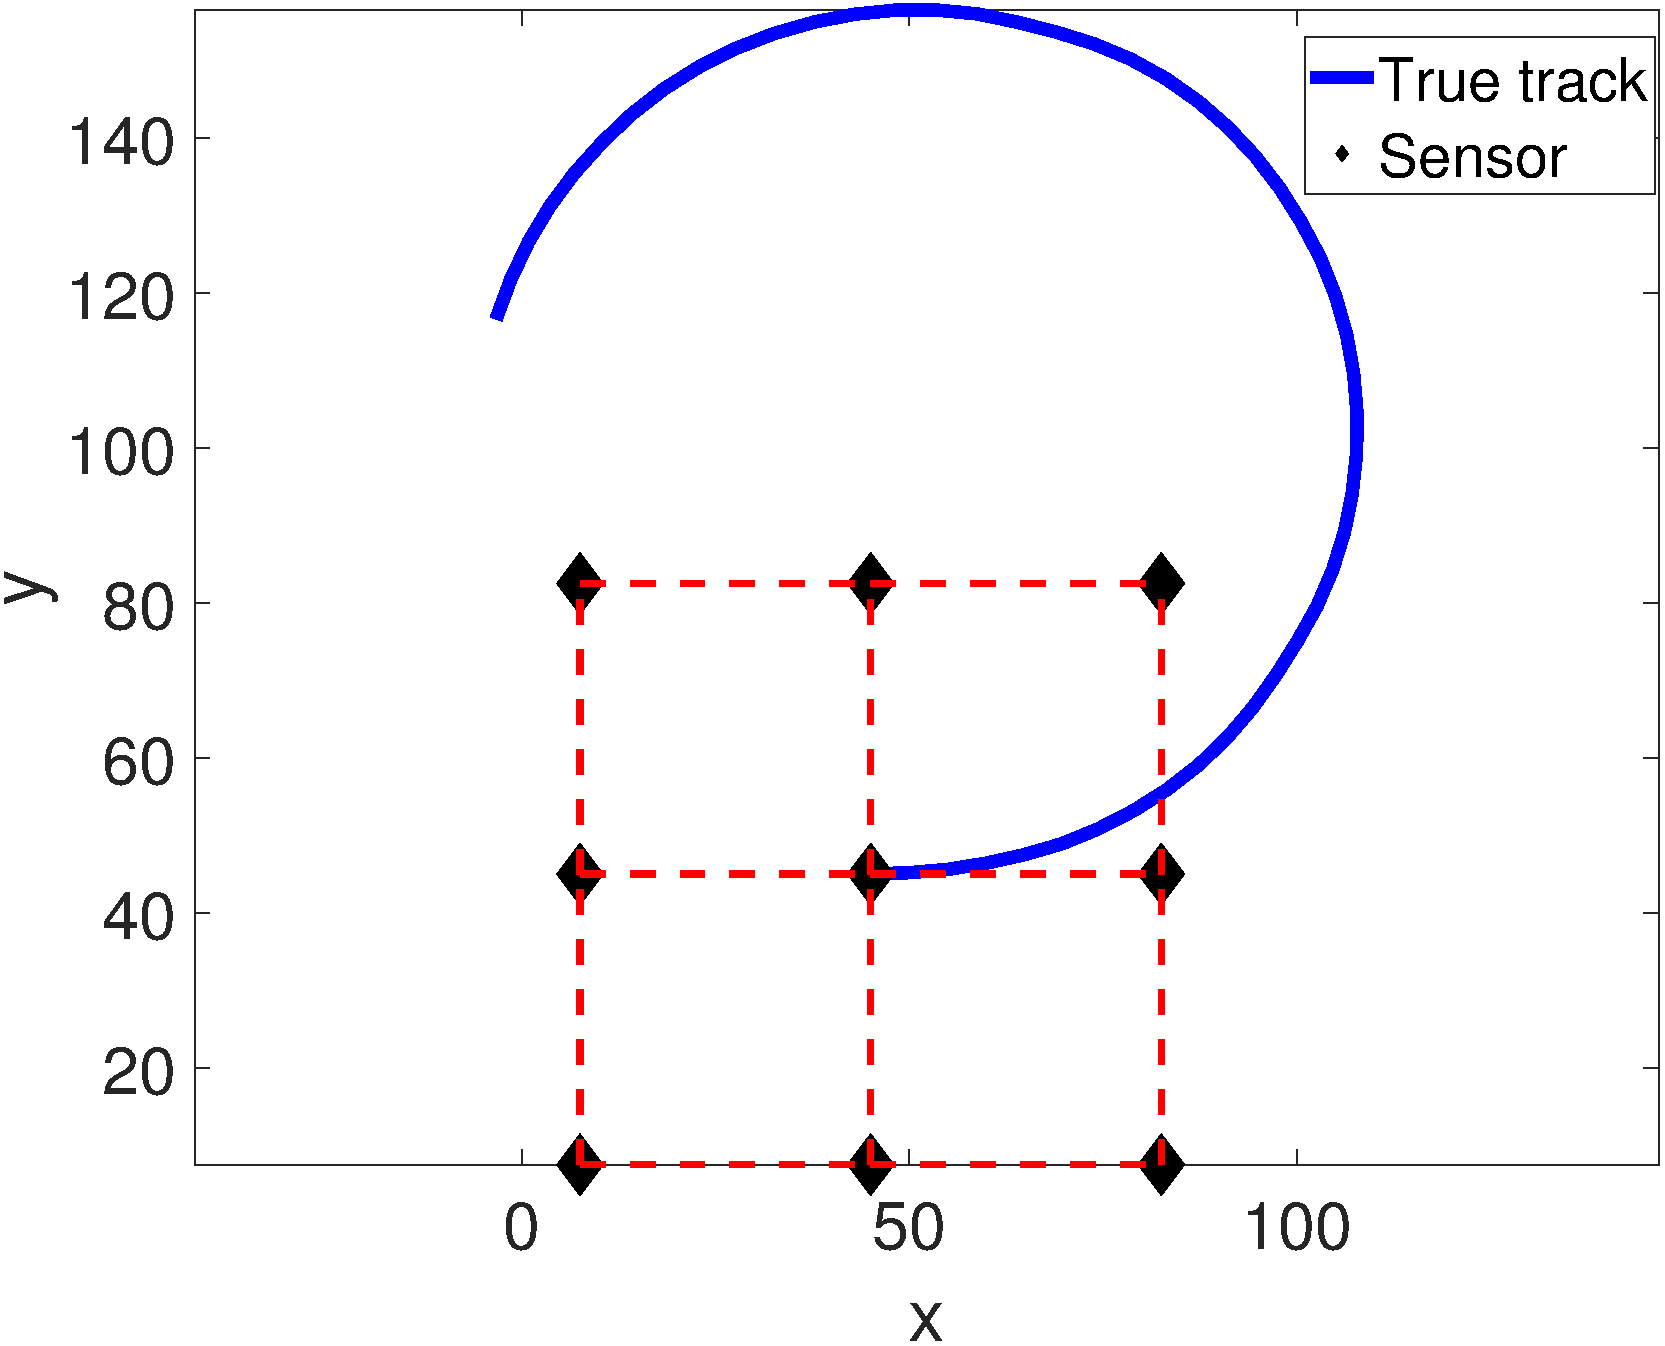
\includegraphics[width=0.45\textwidth]{Figures/track}
\caption{Target trajectory (blue curve) and sensor positions (black diamond). Sensors connected by red dashed lines are within broadcast range of each other.}
\label{fig:track}
\end{figure}

\subsection{Algorithm setup}
All particle filters use a total of $N=500$ particles. At time step 1, we generate the initial particles using the true target state: $X_i(1) \sim \mathcal{N}(X(1), R_{\text{initial}})$ with $R_{\text{initial}}=\text{diag}([0.5^2,0.5^2,0.05^2,0.05^2])$. 

For LCpf, we use a set of basis functions involving all permutations of $x_t^iy_t^j$ with $0\leq i, j \leq d$ where $d$ is some user-specified max degree. For $d=2$, the basis functions would be $\beta_1(X) = x_t^0 y_t^0 = 1, \beta_2(X) = x_t^0 y_t^1 = y_t, ..., \beta_9(X) = x_t^2 y_t^2 $. Note that, due to our choice of basis functions, all particles must remain synchronized across all sensors as in the case of LApf and Clusterpf. For LApf, we construct a DT graph and retain $m< N$ eigenvectors as the basis of Laplacian transformation. For Clusterpf, all particles are grouped into $C$ clusters and a DT graph is constructed to recover individual particle weights. 

The random number generators are synchronized to ensure that the particles remain the same across sensors. Distributed summation is performed using gossip algorithms. At each time step, we perform $NGossip$ gossip iterations. At each gossip iteration, each sensor $i$ broadcasts its local values $G_i$, receives broadcasts from its neighbors, and then updates its local values as a weighted aggregate:
\begin{align}
G_{i,\text{new}} &= w_{ii}G_{i,\text{old}} + \sum_{j\in N_i}w_{ij}G_{j,\text{old}} \\
w_{ij} &=
\begin{cases}
\frac{1}{1+max(d_i, d_j)} \quad j\in N_i \\
1-\sum_{j\in N_i}w_{ij} \quad i=j \\
0 \quad j\notin N_i
\end{cases}
\label{eqn:metropolis_weight}
\end{align}
where $N_i$ denotes the set of neighboring sensors of sensor $i$, $d_i=|N_i|$, and Metropolis weight is used for the update. After a total of $NGossip$ iterations, a max consensus algorithm is run to ensure all sensors obtain the same values. 

In our codes, we do not implement a loop for the gossip iterations. Instead we define an update matrix $W$ where $W(i,j)=w_{ij}$. Therefore, given initial values $G_{\text{initial}}=[G_1,...,G_S]^T$, the final values can be easily computed as 
\begin{equation}
G_{\text{final}} = W^{NGossip}G_{\text{initial}}
\end{equation}

In the remainder of the section, we run a number of Monte Carlo simulations to evaluate the performance of the four filters. The track remains the same in each trial; but the measurements differ. We evaluate the algorithms' performances using two criterion: \textit{root mean squared error} (RMSE) of position estimate, and \textit{aggregate error ratio} (AER). The first metric is self-explanatory; so we will only explain the last one. Let $G_{gossip}$ denote the vector of the approximate aggregate values computed using gossip and max consensus, and let $G_{exact}$ denote the vector of exact aggregate values. We compute the ratio vector $|\frac{G_{gossip}-G_{exact}}{G_{exact}}|$ and report the average ratio. Ideally, for $NGossip$ approaching infinity, the ratio approaches 0 as the approximate value approaches the exact value. 

\subsection{Computational overhead}
In this section we compare the computational overhead of the four filters. More specifically, we compare the overhead for particle log-likelihood computation.

Consider first CSSpf. Each sensor computes the six local sufficient statistics with complexity $O(1)$. These statistics are then aggregated via distributed consensus with complexity $O(S*NGossip)$. Finally, the log-likelihoods are computed at all sensors using the global sufficient statistics with complexity $O(S*N)$. Thus, the overall complexity of CSSpf is thus $O(S+S*NGossip+S*N)$. Since $N>NGossip$ in general, the complexity is dominated by $\underline{O(S*N)}$. 

Consider next LCpf. Let $J$ denote the number of basis functions. Each sensor needs to generate a $N\times J$ matrix to compute the local coefficients. Then $J^2+J$ coefficients are aggregated via distributed consensus over $NGossip$ iterations. The log-likelihoods are finally computed from the global coefficients. The overall complexity is thus $O(S*N*J+S*NGossip*(J^2+J)+S*N) \subset \underline{O(S*N*J+S*NGossip*J^2)}$. 

Consider next LApf. The Delaunay triangulation for graph construction has complexity $O(N\log(N))$. The eigenvalue decomposition has complexity $O(N^3)$. Assume $m$ eigenvectors are used to decode the local log-likelihoods. Then $m$ scalars are aggregated via distributed consensus. The joint log-likelihoods are then recovered from the $m$ aggregate scalars. The overall complexity is thus $O(S*N\log(N)+S*N^3+m*N^2+S*m*NGossip+S*N)\subset \underline{O(S*N^3)}$. 

Finally consider Clusterpf. Particle clustering has complexity $O(N*C*4*I)$ where $I$ is the number of clustering iterations (with default value of 100) and the constant $4$ is the target state dimension. $C$ cluster log-likelihoods are then aggregated across all sensors. We again have Delaunay triangulation for graph construction. The log-likelihood is recovered via convex minimization with complexity $O(\sqrt{N})$. The overall complexity is thus $O(S*N*C*4*I+S*C*NGossip + S*N\log(N)+S\sqrt{N})\subset \underline{O(S*N*C+S*N\log(N))}$

Overall, CSSpf has the lowest overhead and LApf has the highest overhead due to the eigenvalue decomposition. 

\subsection{Constraint sufficient statistics particle filter}
Consider first CSSpf. Each sensor needs to broadcast $6NGossip$ scalars at each time step. We thus study the trade-off between communication overhead and tracking performance. Fig.~\ref{fig:results_CSSpf} shows the boxplots of RMSE and AER with respect to number of gossip iterations for different values of $N$. Each data point is averaged over 50 time steps and 200 Monte Carlo trials. 

The RMSE is very high for $NGossip=10$ which can be attributed to the gossip algorithms not converging in such few iterations and leading to high errors in the final values of the global sufficient statistics. For $NGossip\geq 20$, the RMSE is fairly constant and more gossip iterations and more particles do not yield significant improvement in tracking performance. 

%The runtime does not increase with higher $NGossip$ due to our implementation of the gossip algorithms. When $N$ increases, the runtime increases as expected. 

With increasing $NGossip$, the AER decreases exponentially (note the log-scale of the Y-axis). For $NGossip=20$, the ratio drops close to 0.02 which is low enough to yield adequate tracking performance. For higher values of $NGossip$, the ratio drops even further; although the tracking performance improvement is marginal at best. As $N$ increases, the AER does not change significantly. This is to be expected since the number of sufficient statistics to be aggregated is constant and independent of the number of particles. 

\begin{figure}
\centering
\begin{subfigure}[RMSE]
{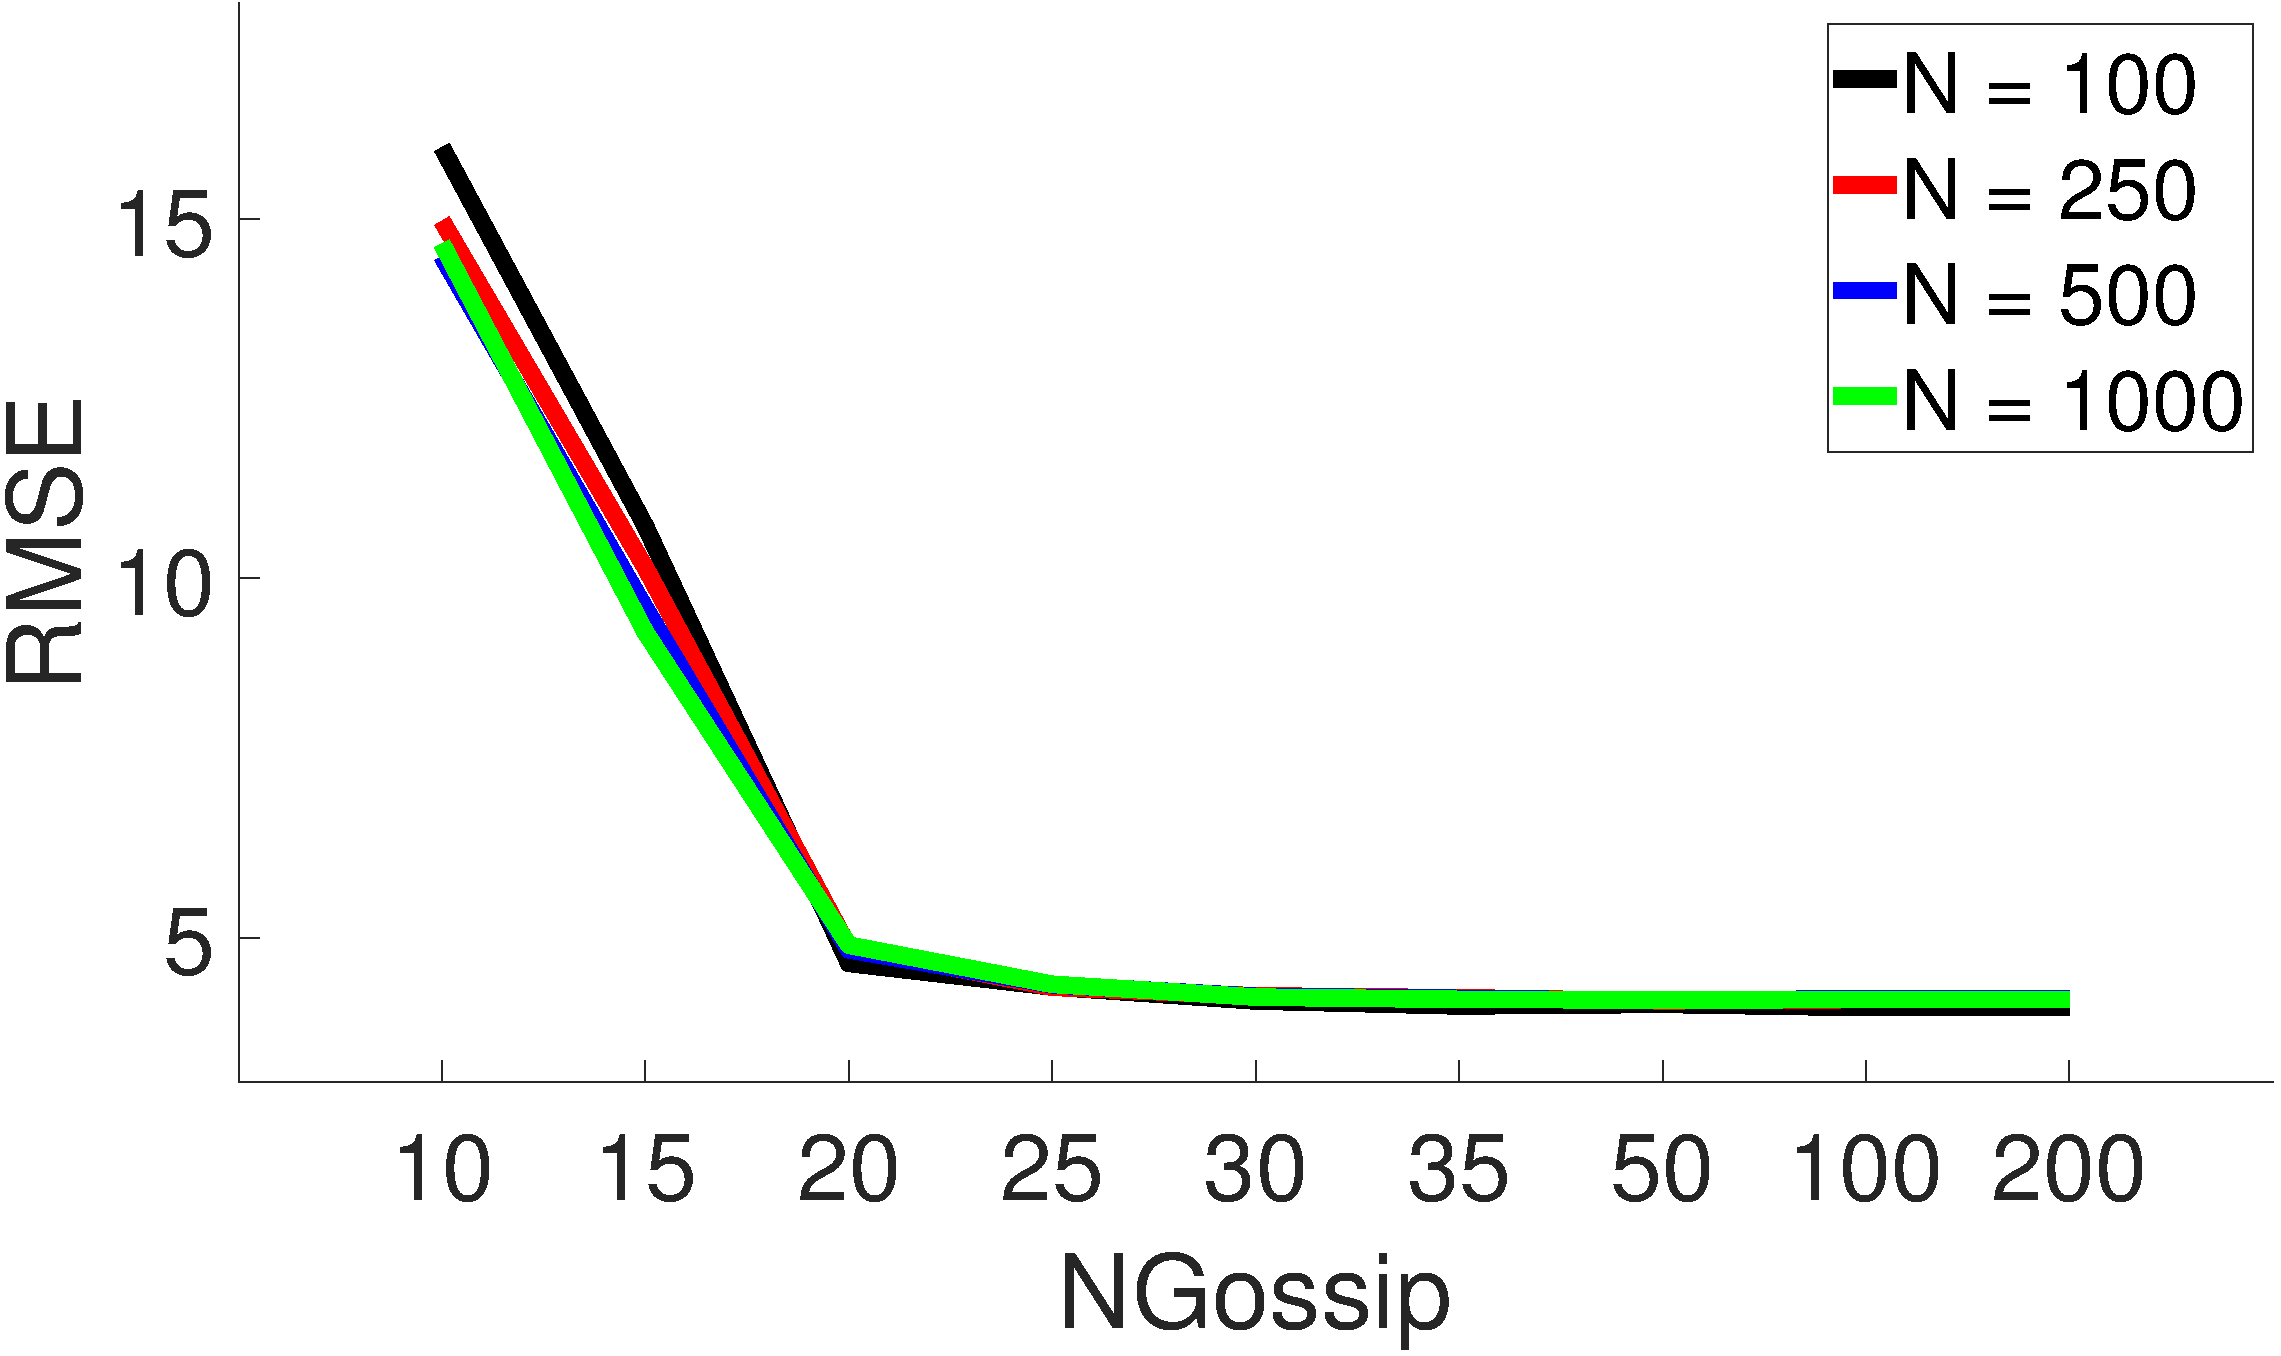
\includegraphics[width=0.49\textwidth]{Figures/curve_CSSpf_RMSE}}
\end{subfigure}
%\begin{subfigure}[total runtime]
%{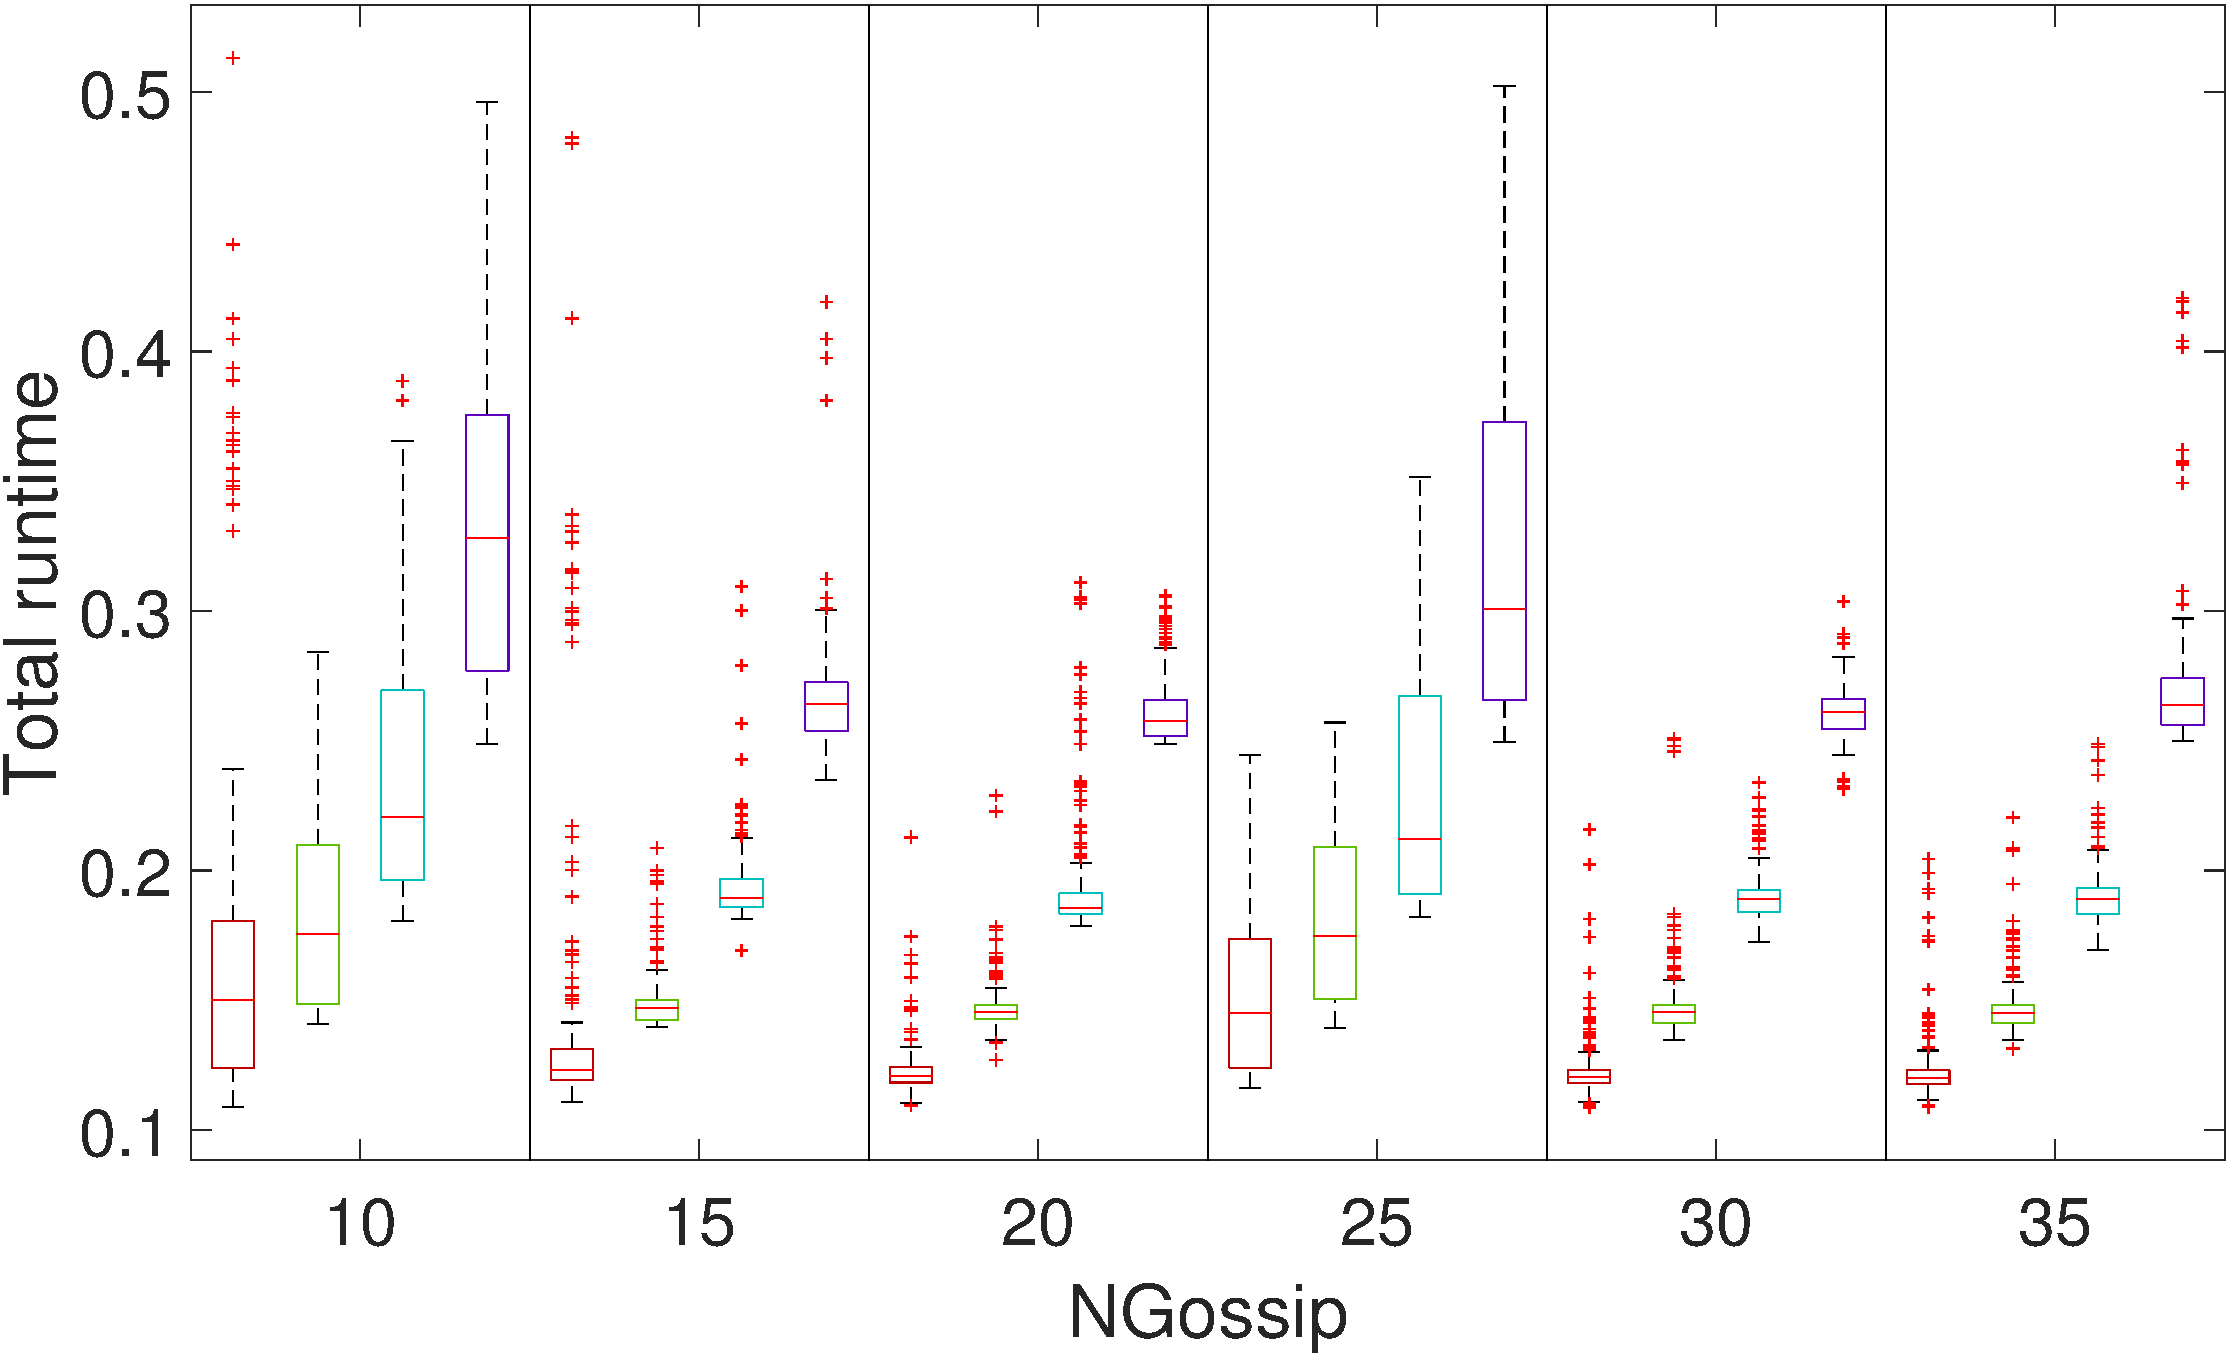
\includegraphics[width=0.65\textwidth]{Figures/boxplot_CSSpf_time}}
%\end{subfigure}
\begin{subfigure}[AER]
{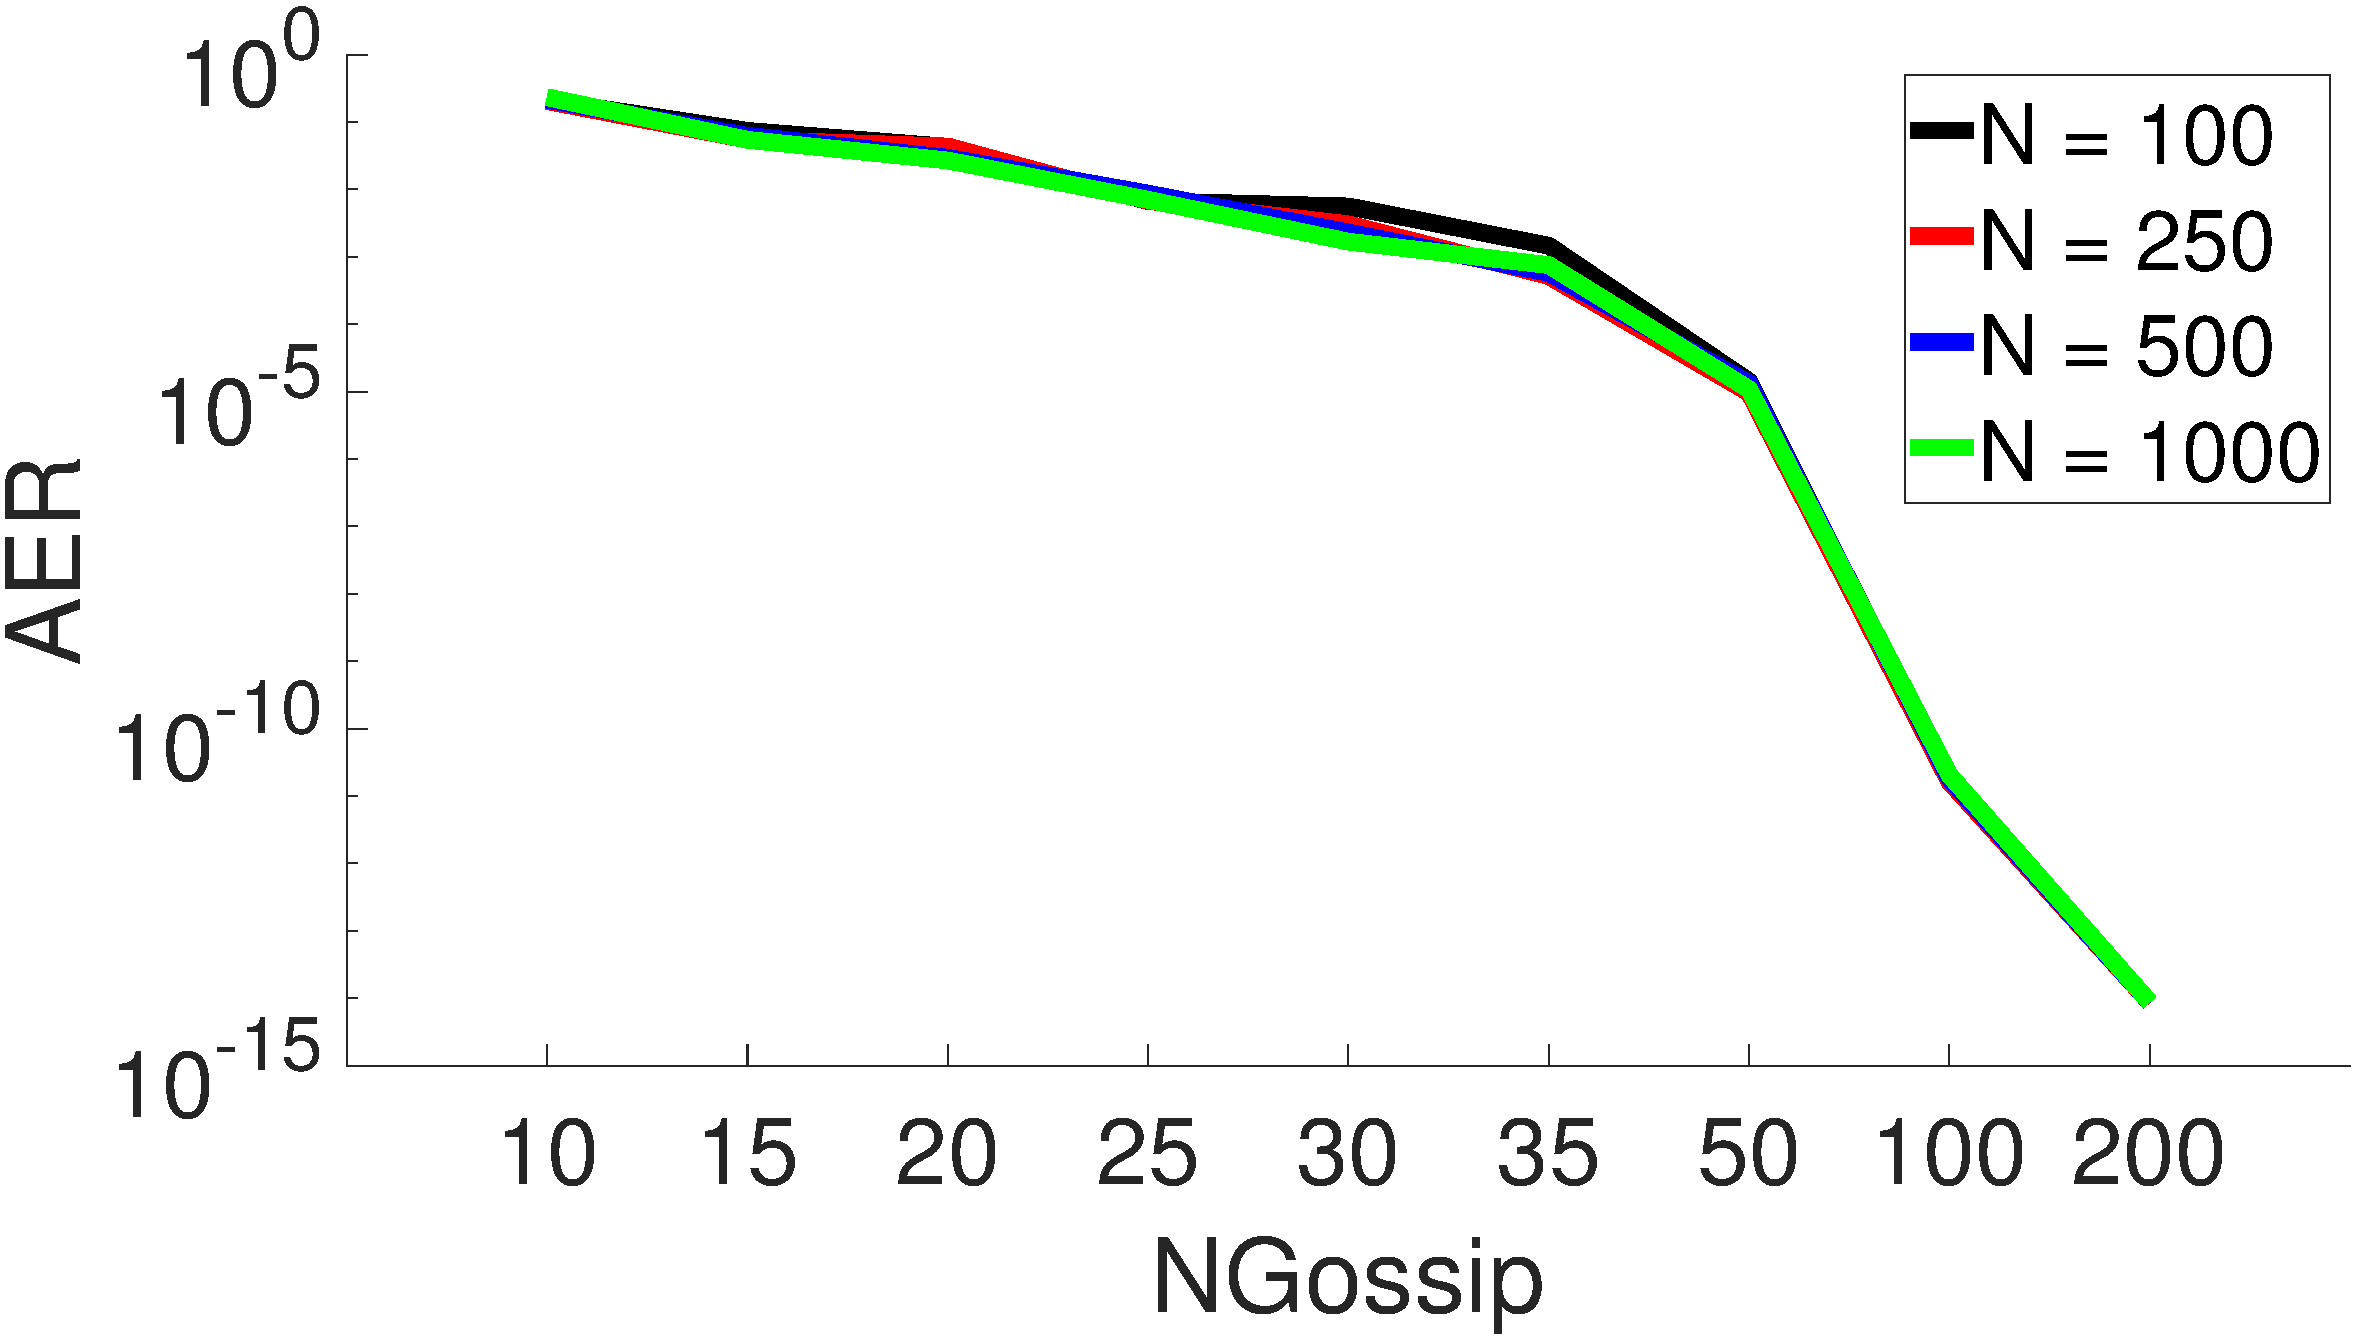
\includegraphics[width=0.49\textwidth]{Figures/curve_CSSpf_AER}}
\end{subfigure}
\caption{RMSE and AER of CSSpf with respect to $NGossip$ for different values of $N$. Each data point is averaged over 50 time steps and 200 Monte Carlo trials.}
\label{fig:results_CSSpf}
\end{figure}

\subsection{Likelihood consensus particle filter}
The max degree $d$ offers a trade-off between tracking performance and computational/communication overhead. Higher degree $d$ generates more basis functions and should yield better approximation of the measurement model. On the other hand, more basis functions lead to more computation, more communication and longer runtime. In fact, the total number of basis functions grows exponentially at $O(d^2)$ and the number of broadcast scalars grows at $O(d^4)$. 

Fig.~\ref{fig:results_LCpf_maxDegree} shows the boxplots of RMSE and total runtime with respect to $d$. Note that, for this particular set of trials, all summations are computed exactly without gossiping. The runtime increases for higher $d$ due to the additional computational overhead as expected. For all values of $d$, the RMSE remains fairly constant. This suggests that additional basis functions from $d\geq 1$ do not improve the approximation of the measurement model $H(X_i)$ by any significant margin. To confirm our conjecture, we compute the following metric. Let $H_{true}(X_i)$ denote the expected measurement of particle $X_i$ and let $H_{approx}(X_i)$ denote the approximate value computed using the basis functions. We then compute the measurement model approximation error $|H_{exact}(X_i)-H_{approx}(X_i)|$ averaged over all particles, all sensors and all time steps. Fig.~\ref{fig:boxplot_LCpf_meas_approx_error} shows the boxplot of average measurement model approximation error with respect to $d$. While the average error does fluctuate somewhat with respect to $d$, the error remains very small in all cases (less than 1 degree) compared to the standard deviation of measurement noise (5 degrees). These results suggest that $d=1$ is sufficient to yield adequate tracking performance while minimizing computational overhead. 

\begin{figure}
\centering
\begin{subfigure}[RMSE]
{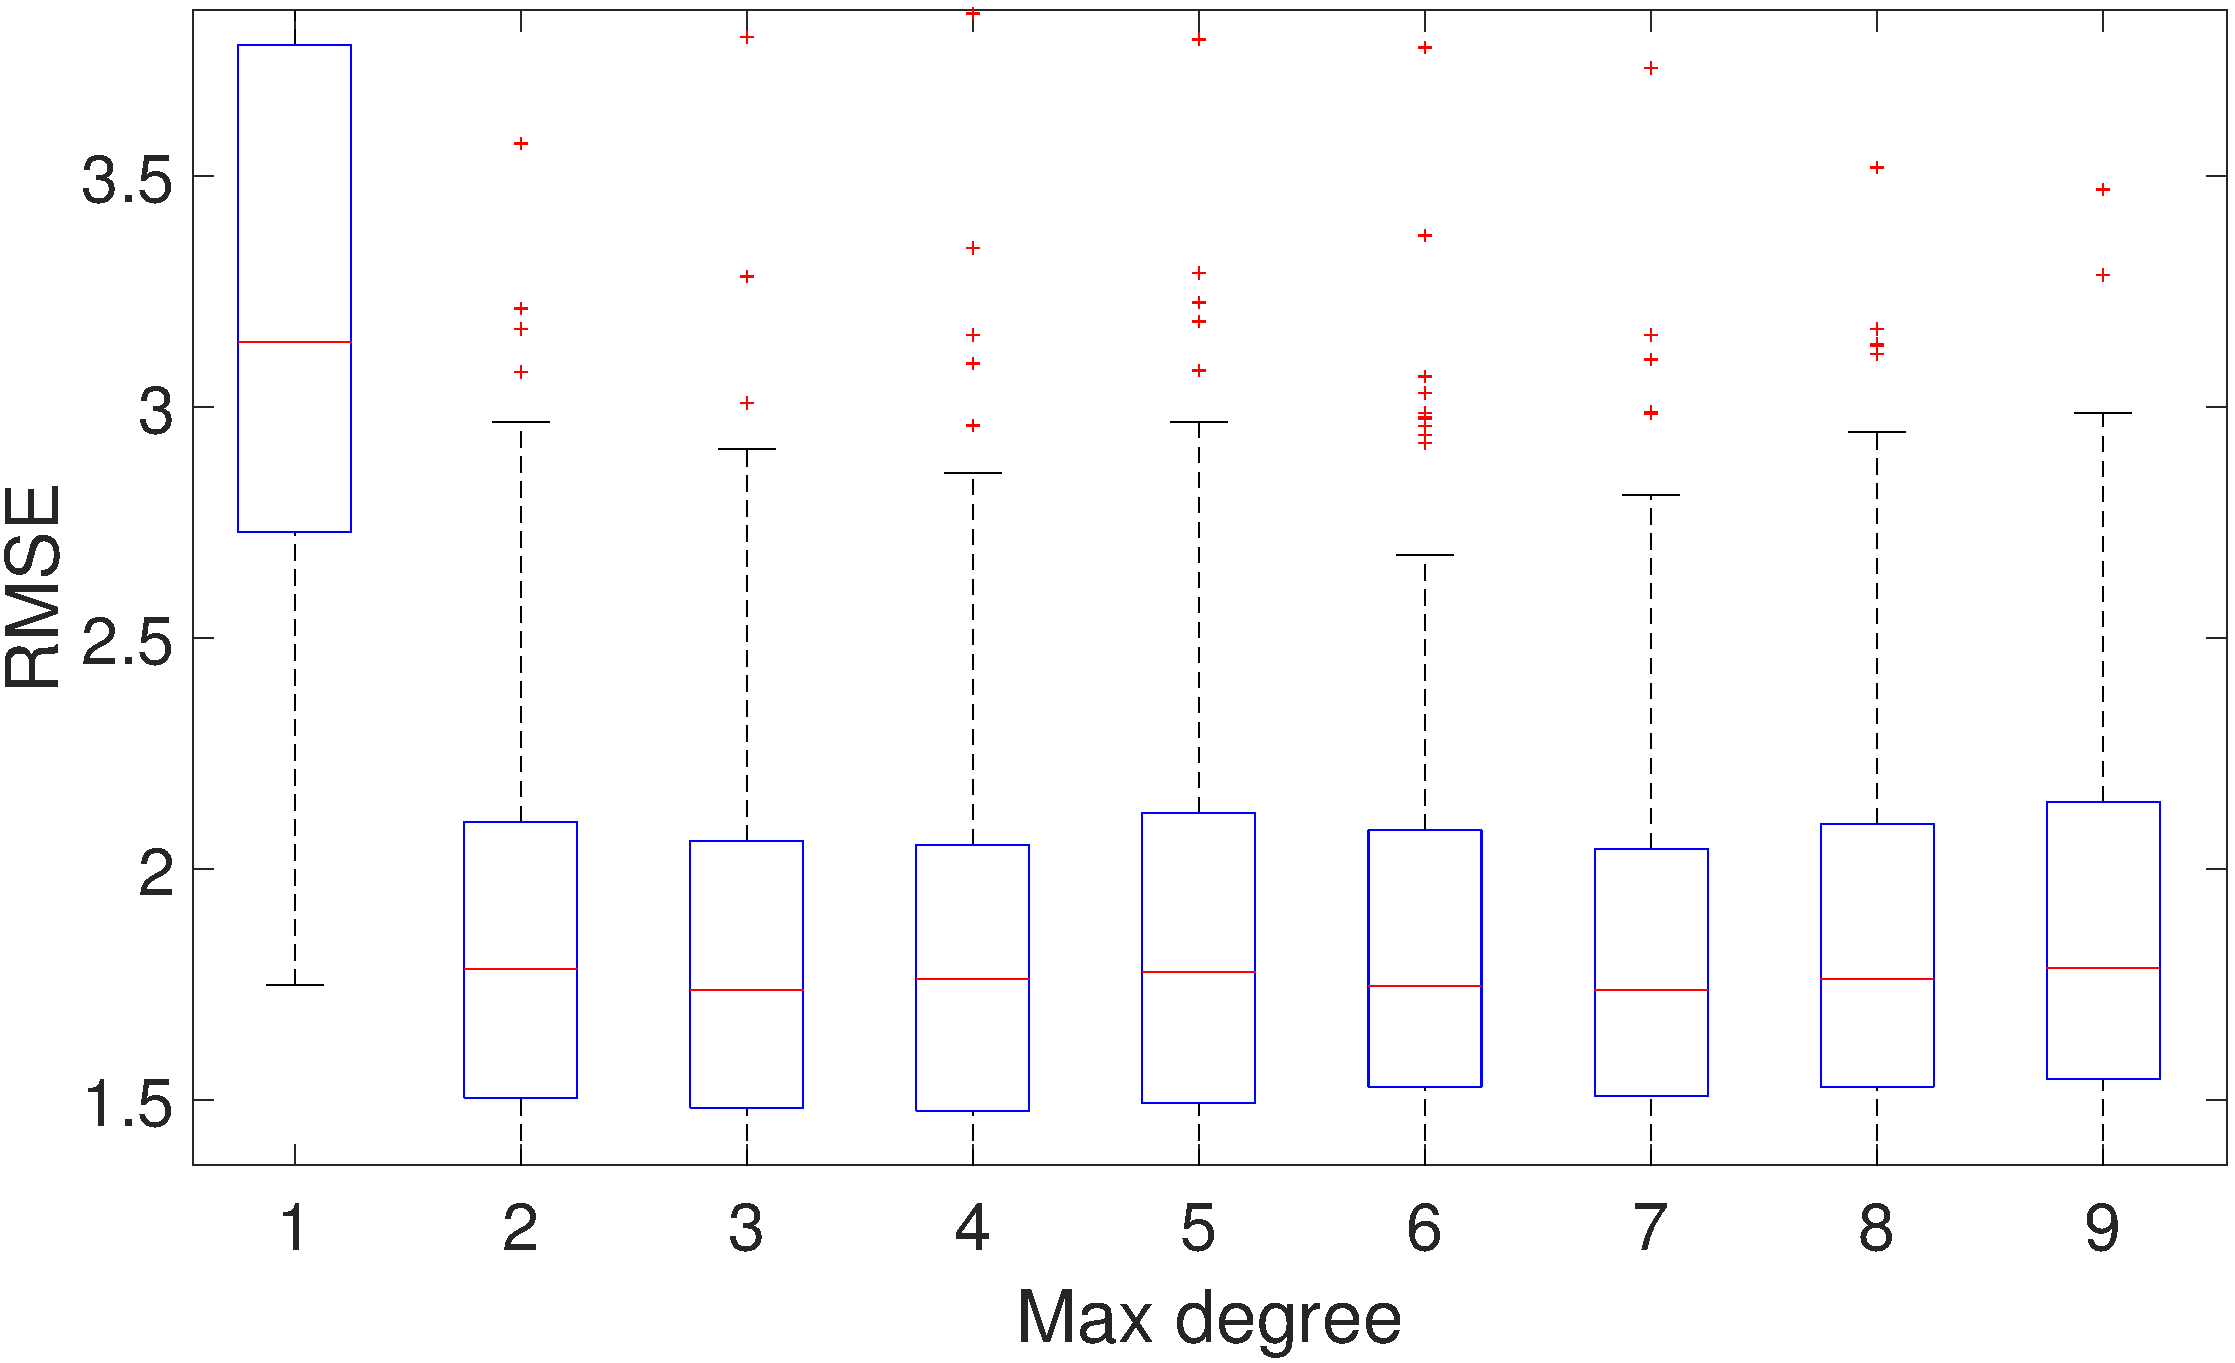
\includegraphics[width=0.49\textwidth]{Figures/boxplot_LCpf_RMSE_maxDegree}}
\end{subfigure}
\begin{subfigure}[total runtime]
{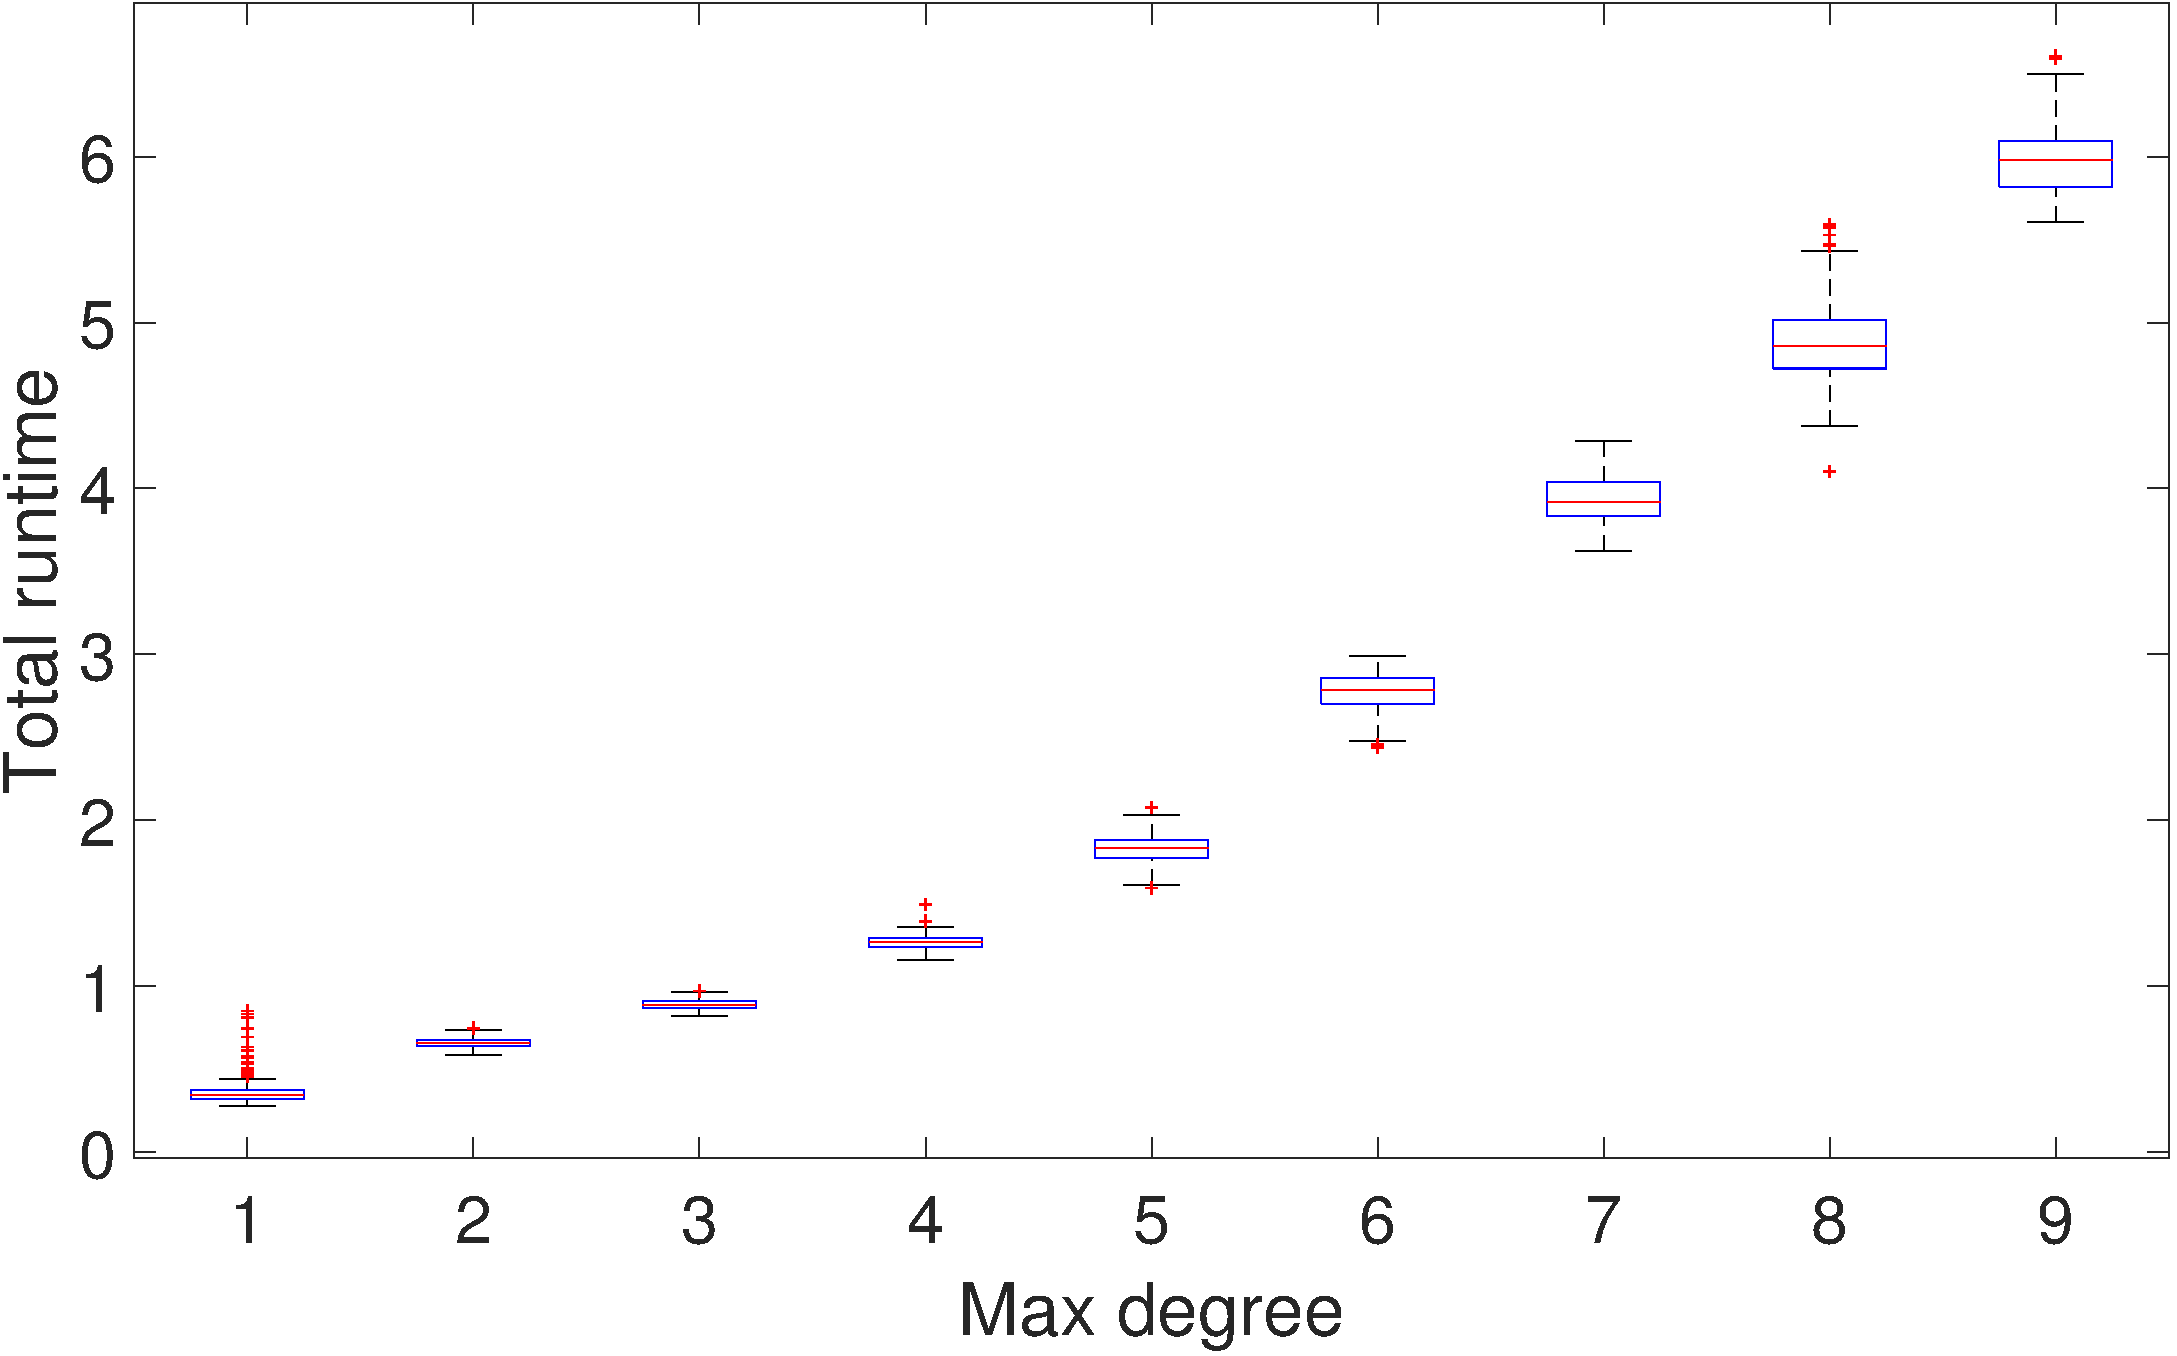
\includegraphics[width=0.49\textwidth]{Figures/boxplot_LCpf_time_maxDegree}}
\end{subfigure}
\begin{subfigure}[Measurement approximation error]
{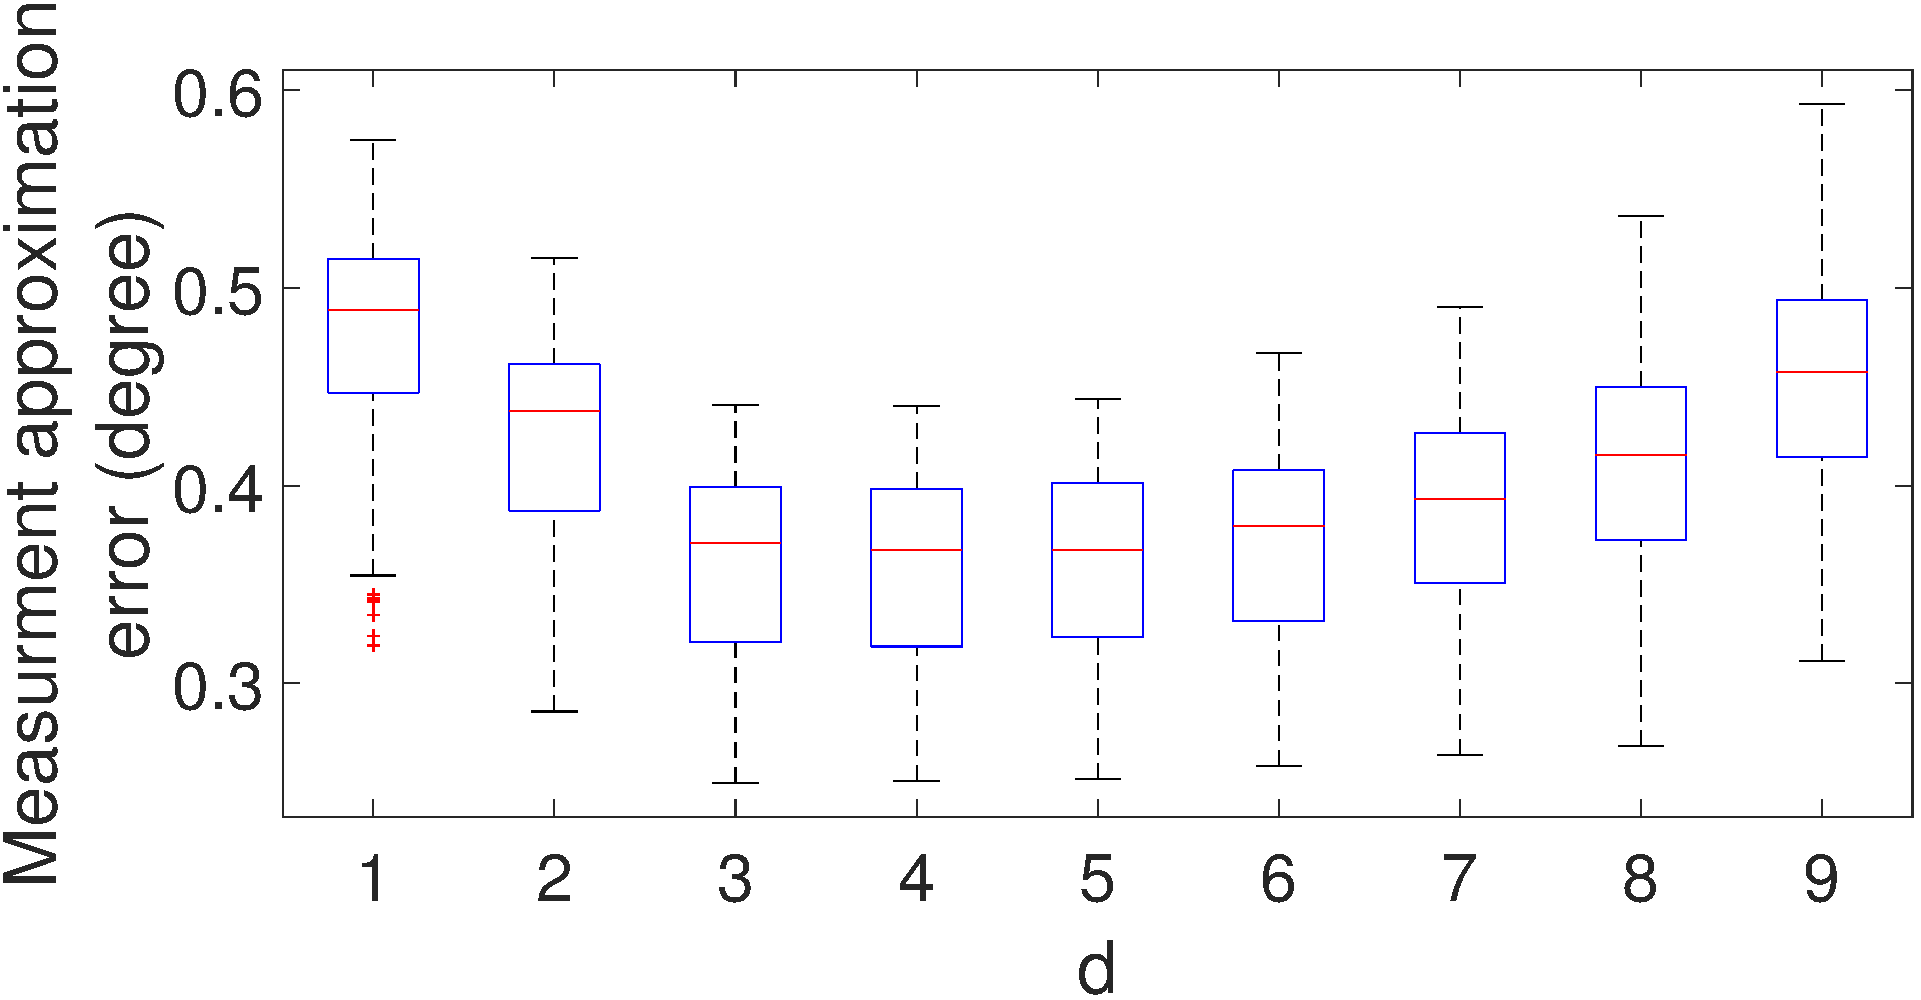
\includegraphics[width=0.49\textwidth]{Figures/boxplot_LCpf_mea_approx_error_maxDegree}\label{fig:boxplot_LCpf_meas_approx_error}}
\end{subfigure}
\caption{Boxplot of RMSE, total runtime and average measurement approximation error of LCpf with respect to $d$. All summations are computed exactly without gossip. $N=500$}
\label{fig:results_LCpf_maxDegree}
\end{figure}

\begin{figure}
\centering
\begin{subfigure}[RMSE]
{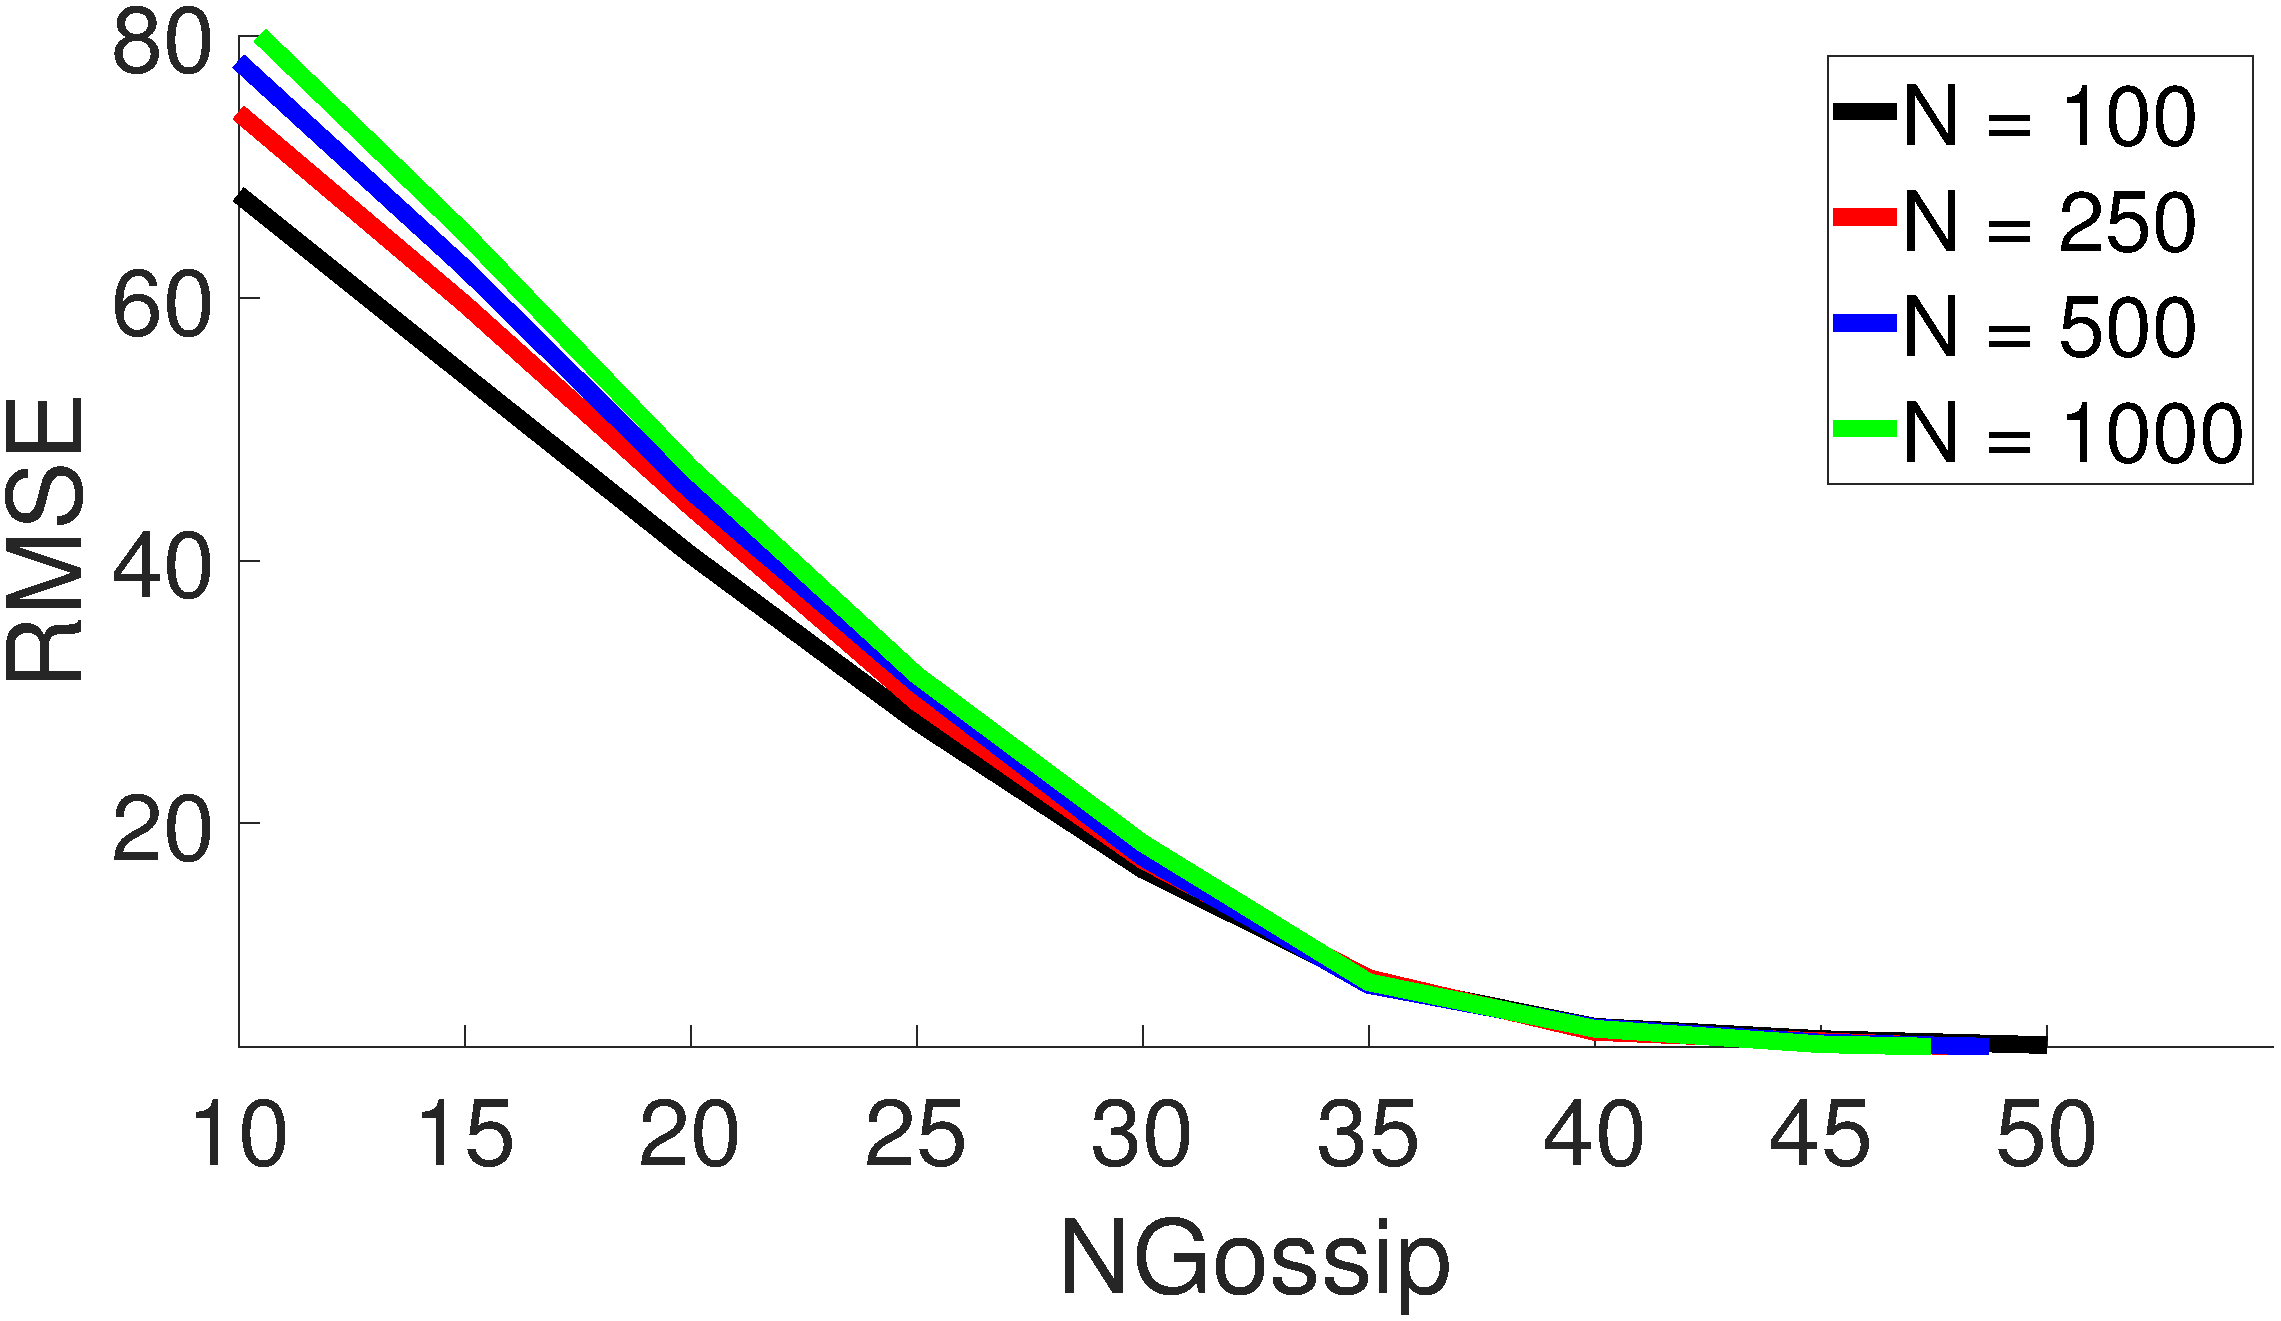
\includegraphics[width=0.49\textwidth]{Figures/curve_LCpf_RMSE}}
\end{subfigure}
%\begin{subfigure}[total runtime]
%{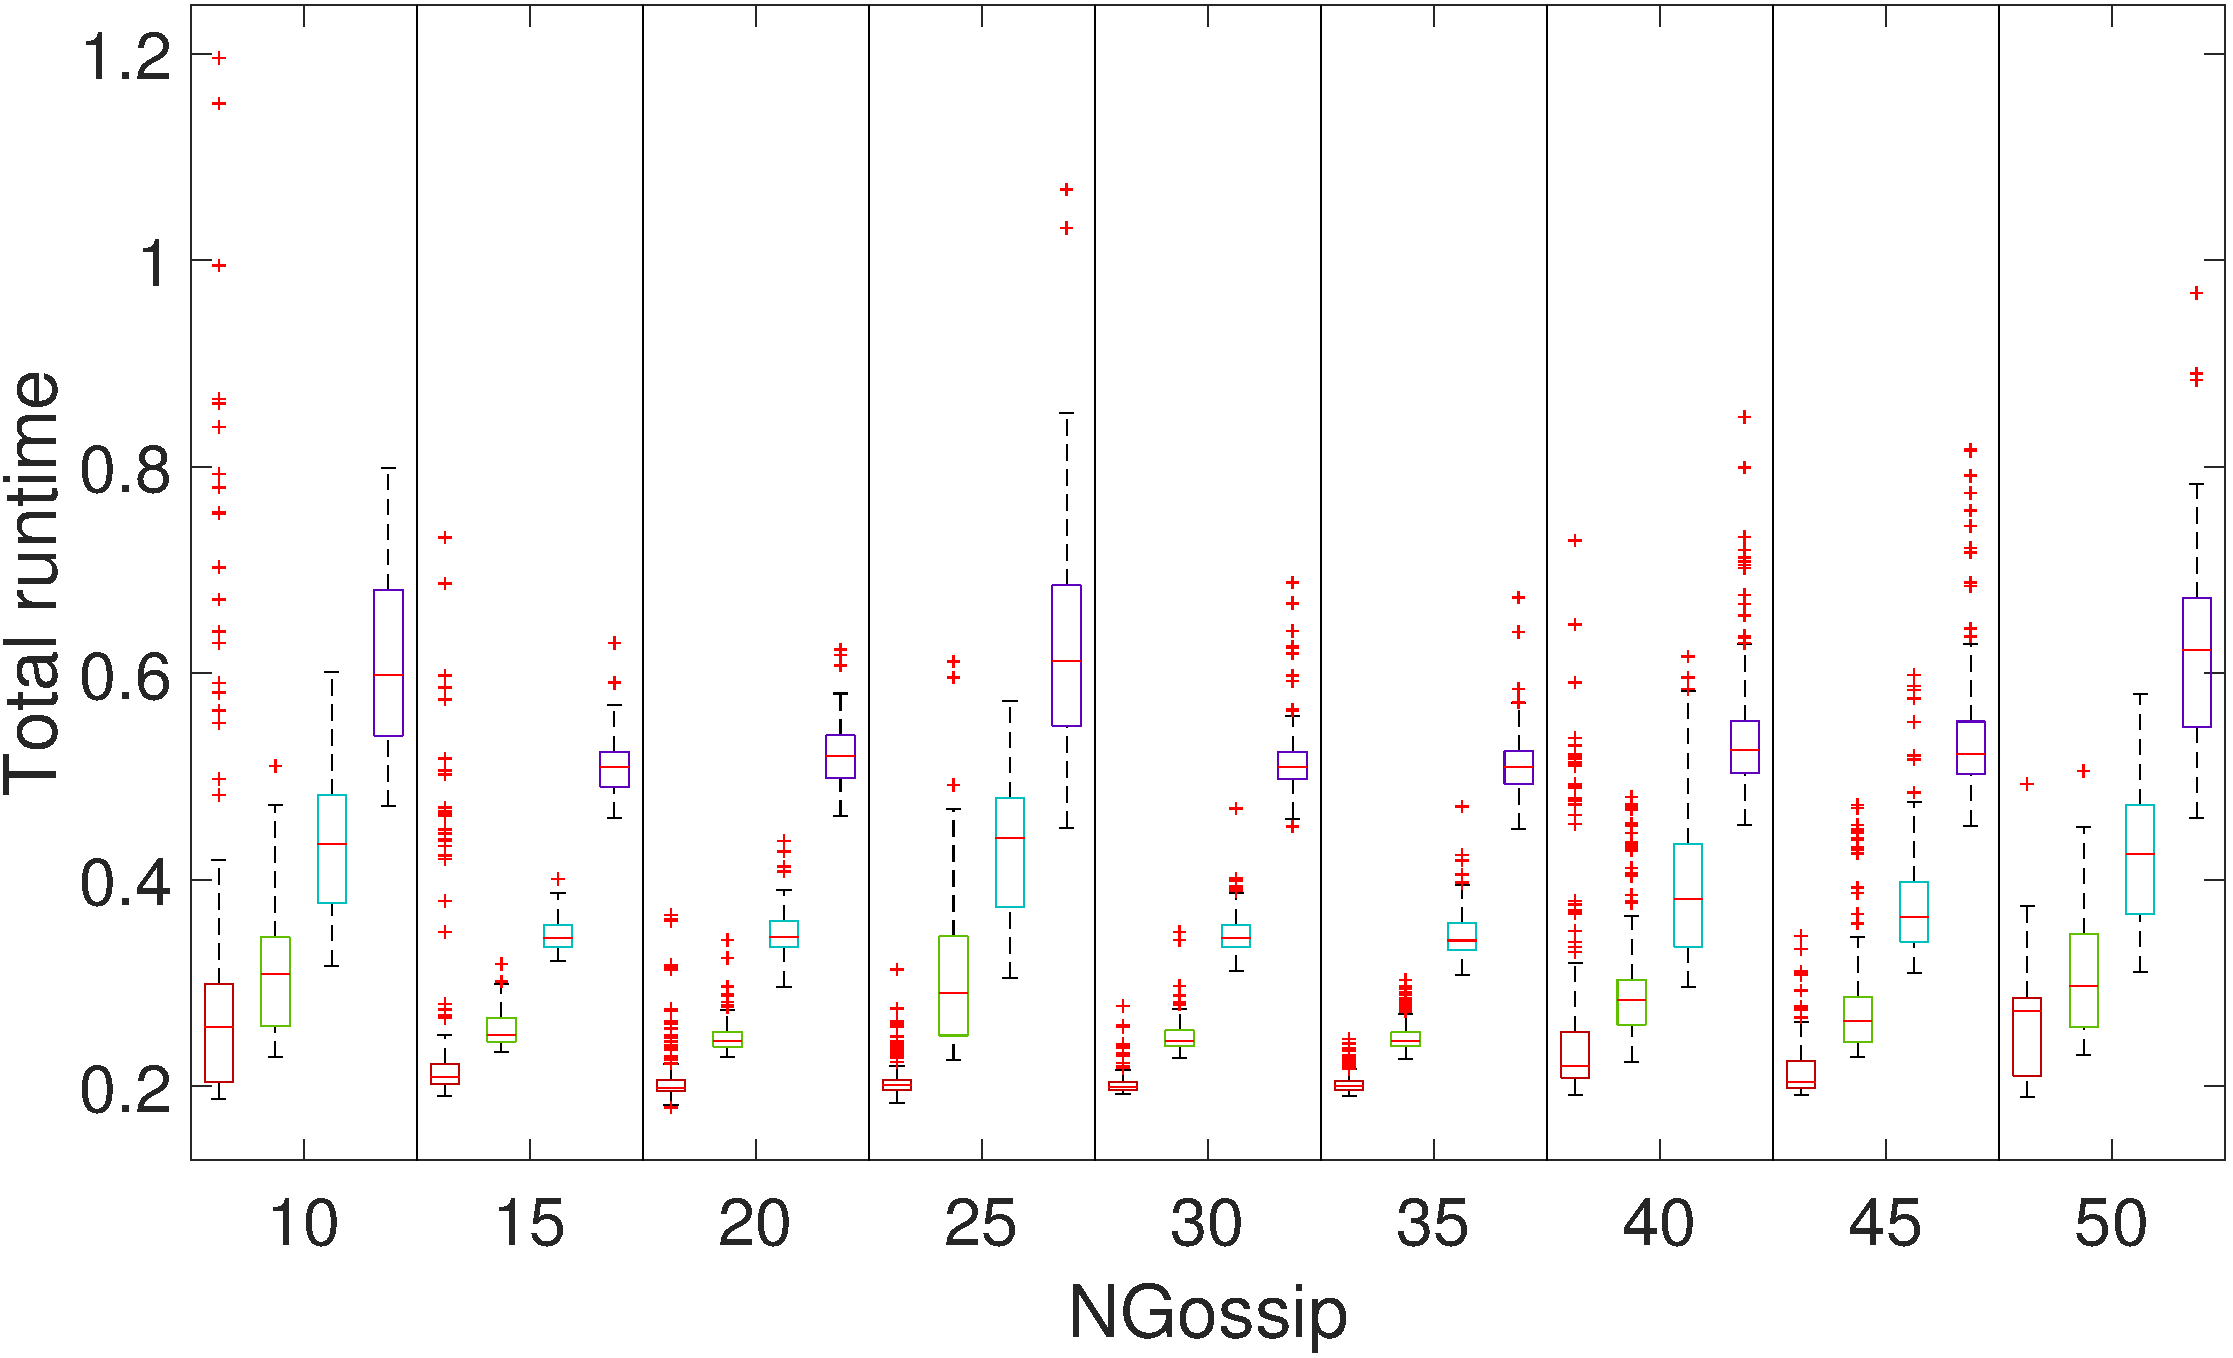
\includegraphics[width=0.65\textwidth]{Figures/boxplot_LCpf_time}}
%\end{subfigure}
\begin{subfigure}[AER]
{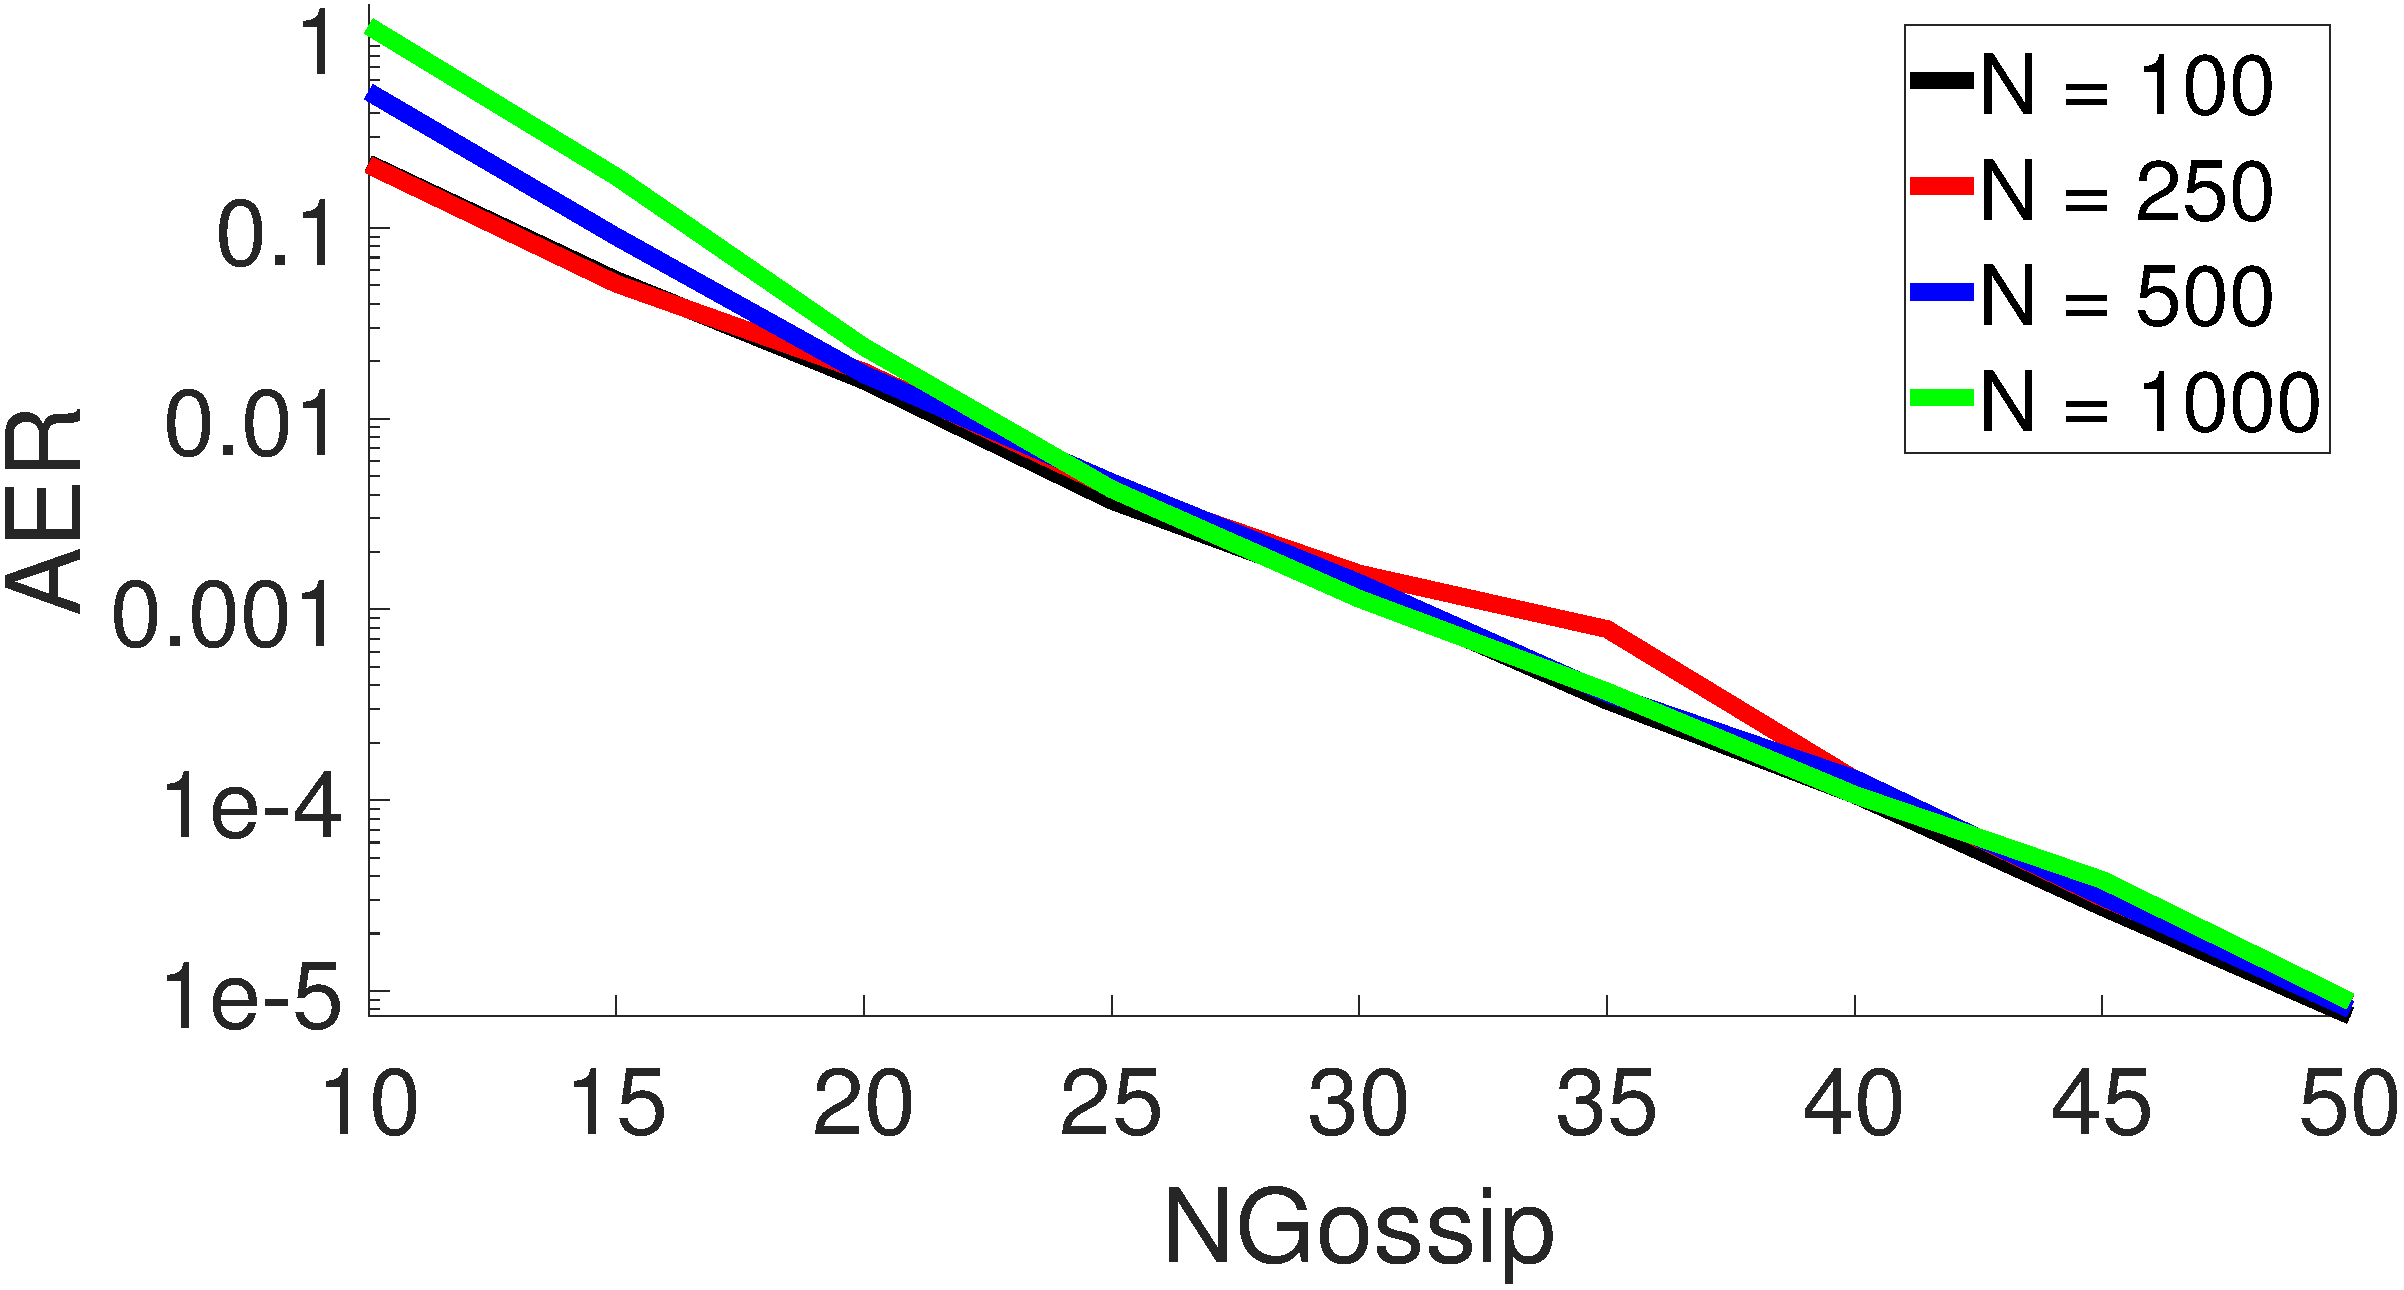
\includegraphics[width=0.49\textwidth]{Figures/curve_LCpf_AER}}
\end{subfigure}
\caption{RMSE AER of LCpf with respect to $NGossip$ for different values of $N$. All data points are averaged over 50 time steps and 200 Monte Carlo trials.}
\label{fig:results_LCpf}
\end{figure}

Fig.~\ref{fig:results_LCpf} shows the boxplots of RMSE and AER with respect to number of gossip iterations for $d=1$ and different values of $N$. Each data point is averaged over 50 time steps and 200 random trials. For LCpf, a minimal of 40 gossip iterations is necessary to yield adequate tracking performance. Furthermore, at $d=1$, each sensor needs to broadcast 20 scalars per gossip iteration. In other words, the communication overhead of LCpf is 6 times that of CSSpf (thrice the scalars to aggregate and twice as many gossip iterations) to achieve similar tracking performance as CSSpf. If we compare Fig. 2(b) and Fig. 4(b), we note that CSSpf and LCpf exhibit very similar level of AER for the same $NGossip$. This suggests that LCpf is significantly more susceptible to error induced by distributed summation. %Furthermore, LCpf requires double the runtime of CSSpf with the total runtime increasing for higher $N$. 

\subsection{Laplacian approximation particle filter}
\begin{figure}
\centering
\begin{subfigure}[RMSE]
{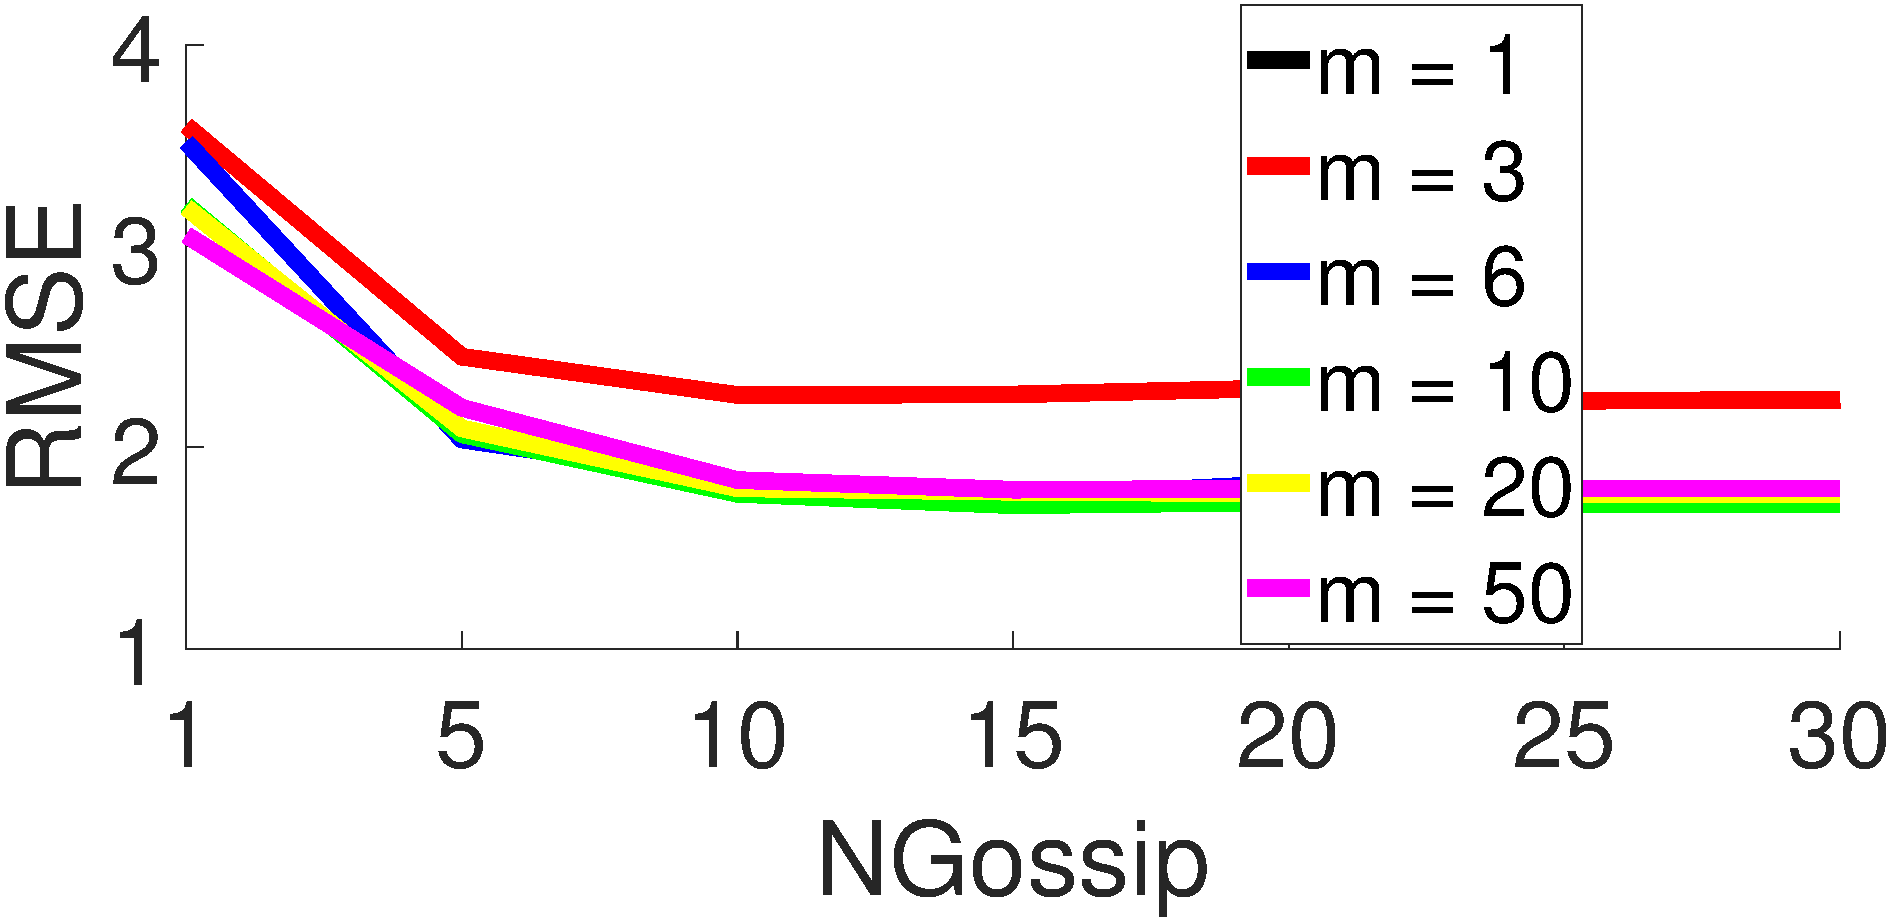
\includegraphics[width=0.49\textwidth]{Figures/curve_LApf_RMSE}}
\end{subfigure}
%\begin{subfigure}[total runtime]
%{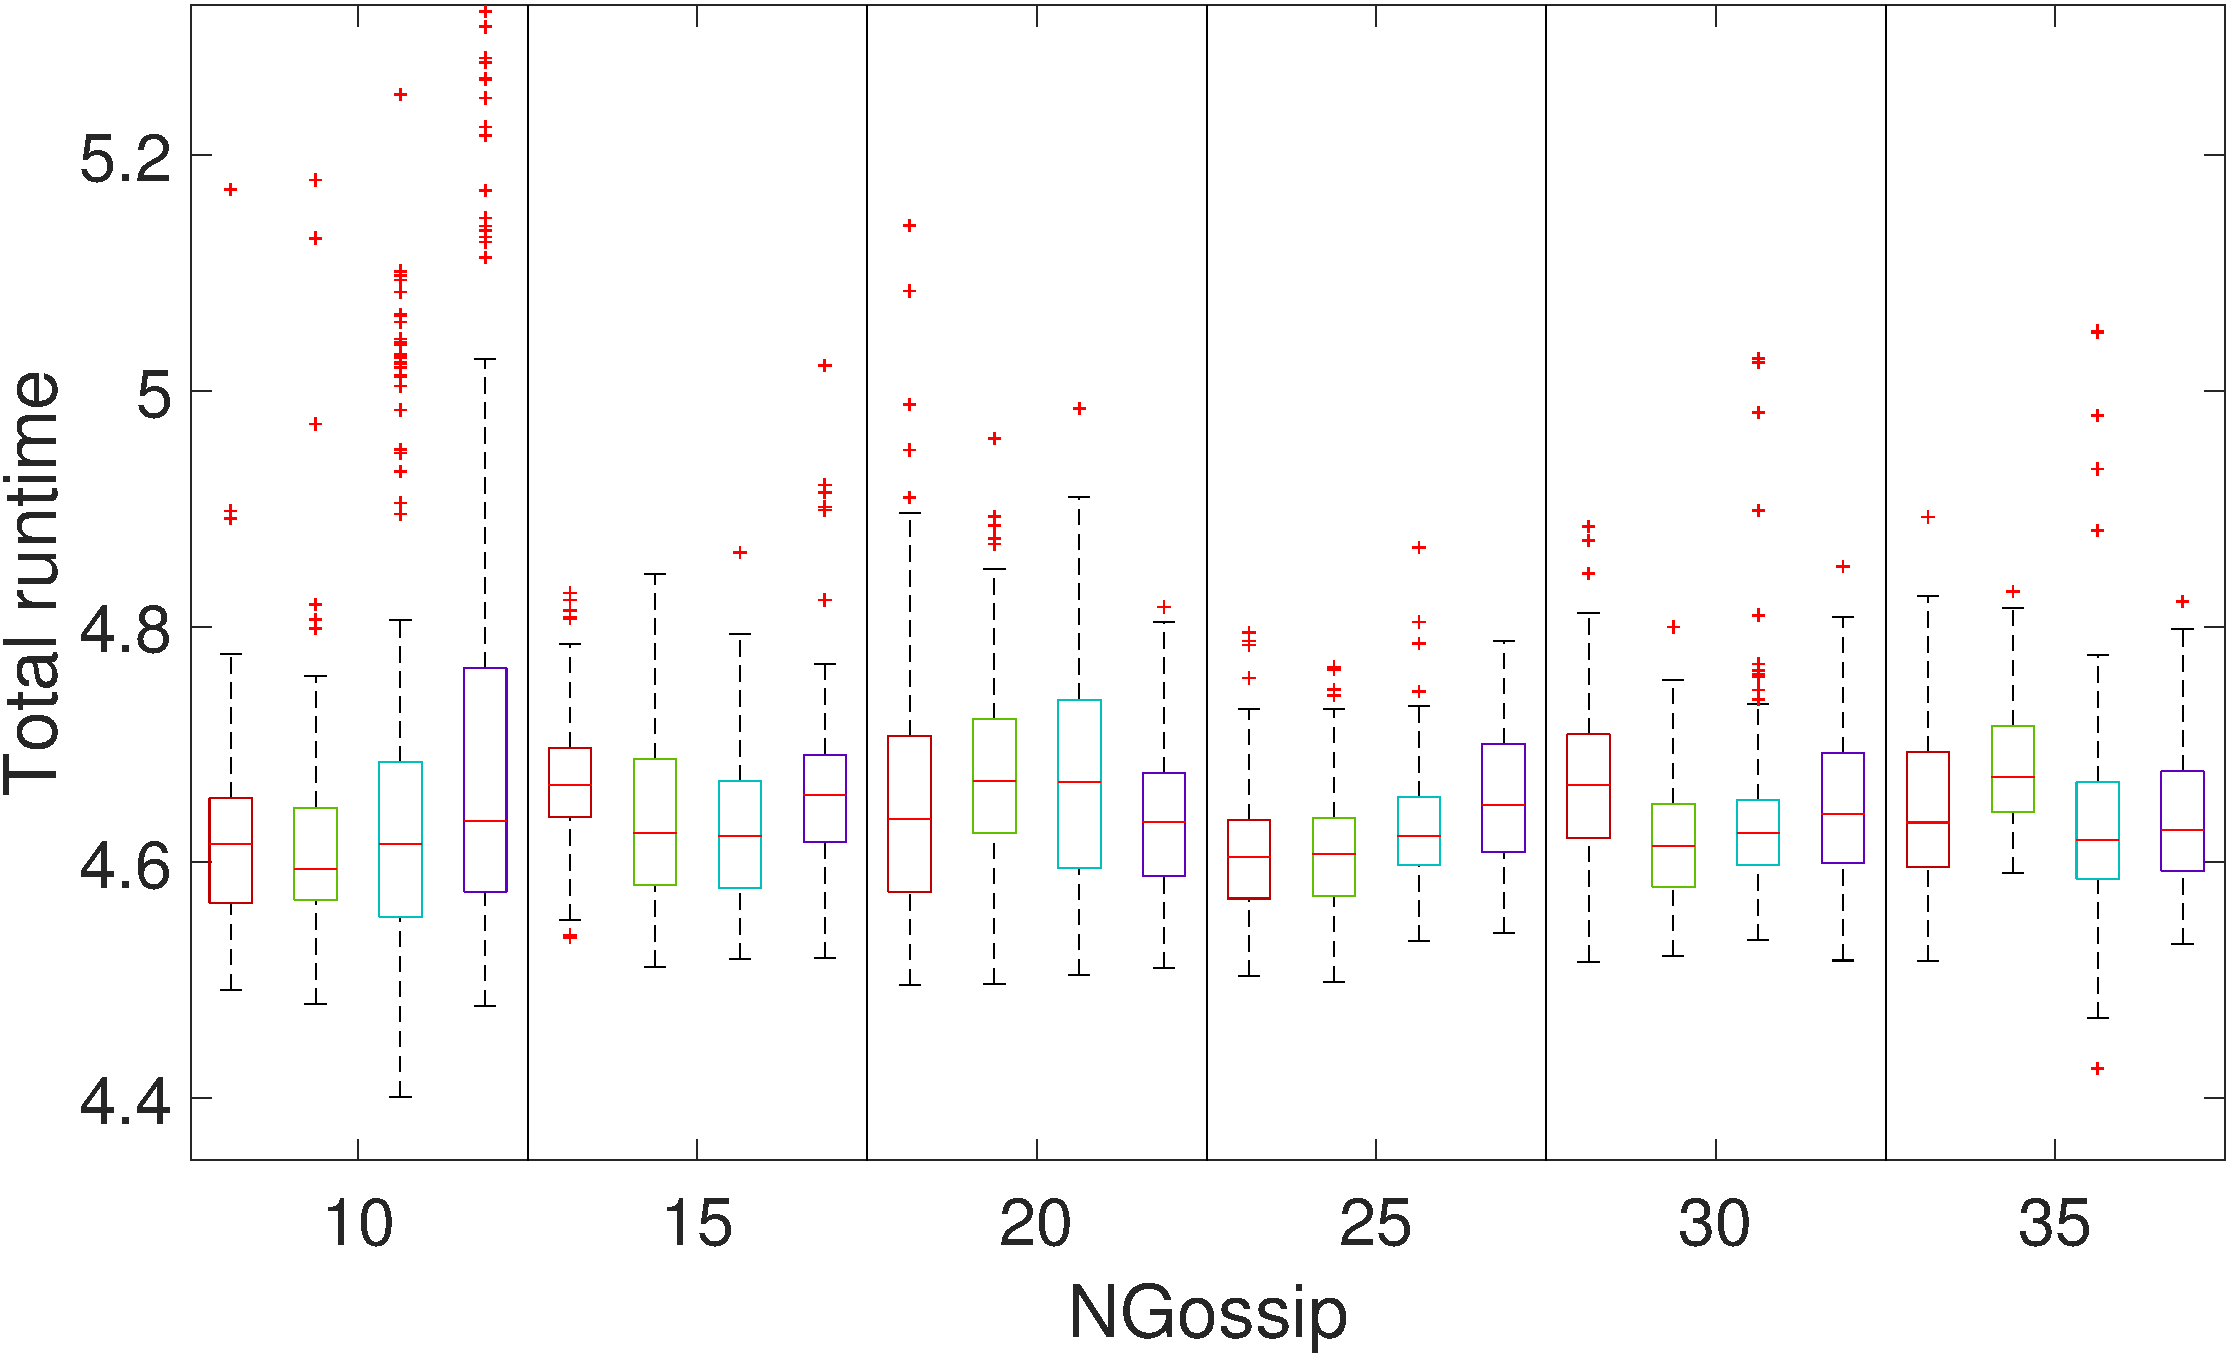
\includegraphics[width=0.65\textwidth]{Figures/boxplot_LApf_time}}
%\end{subfigure}
\begin{subfigure}[AER]
{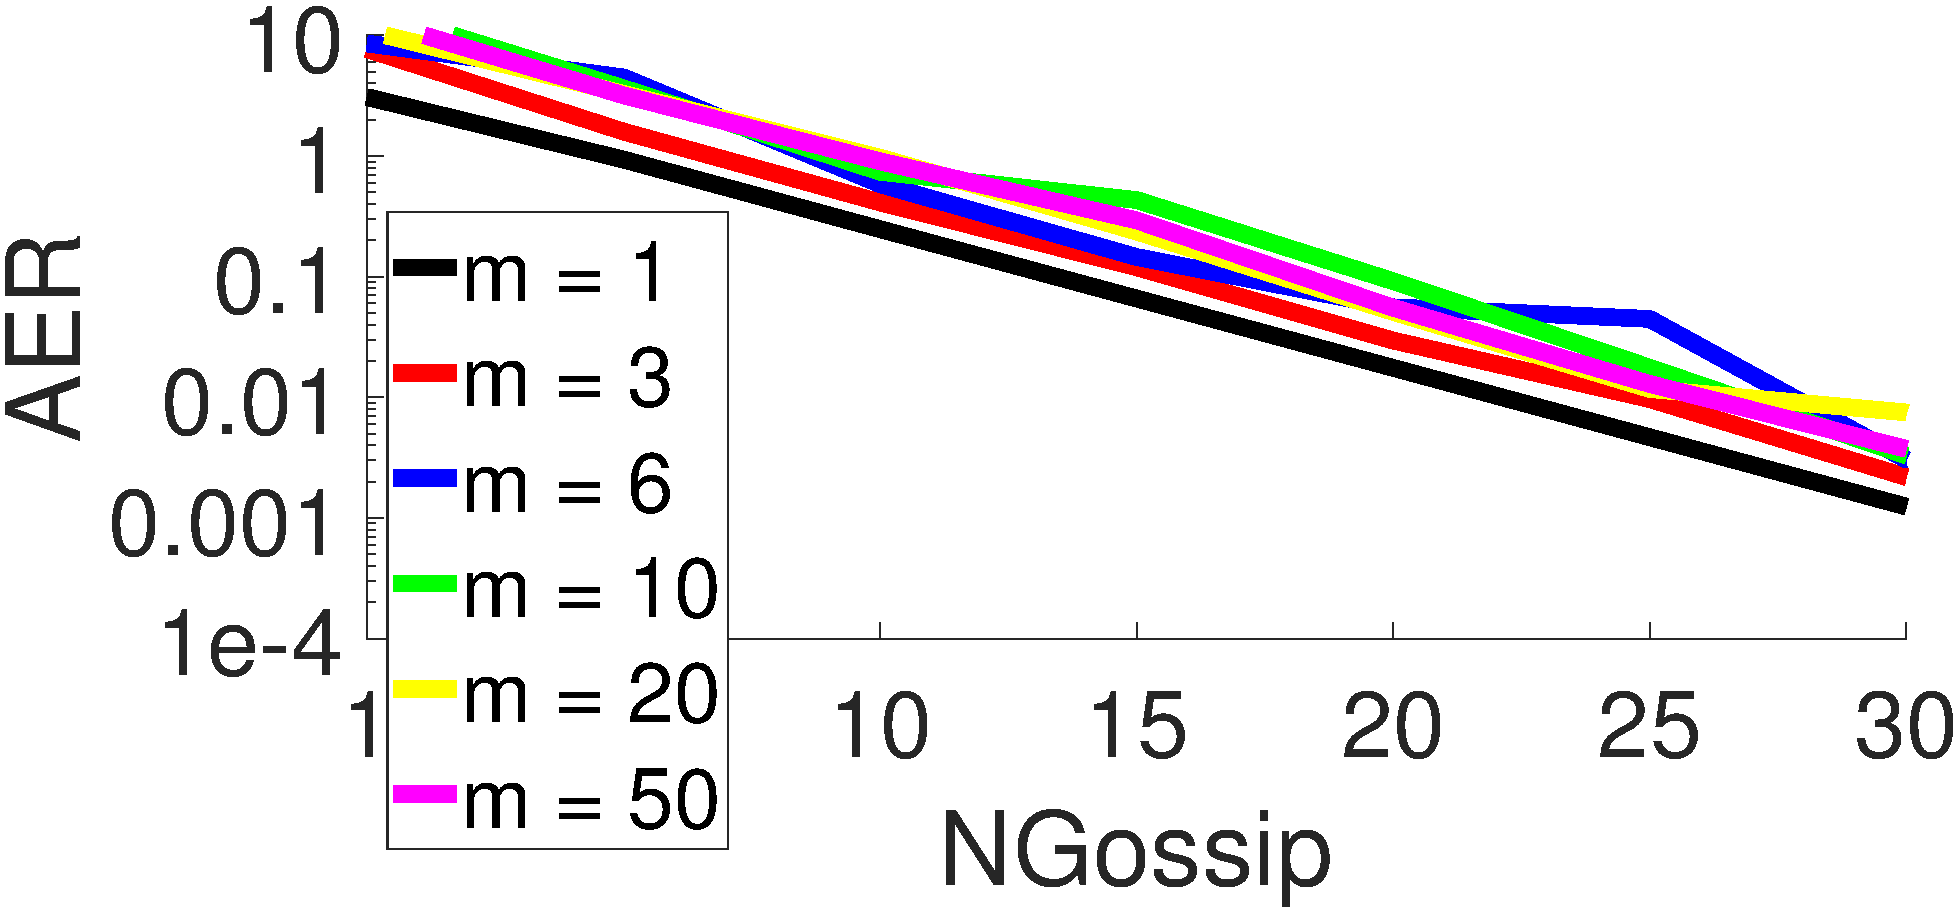
\includegraphics[width=0.49\textwidth]{Figures/curve_LApf_AER}}
\end{subfigure}
\caption{RMSE and AER of LApf with respect to $NGossip$ for $N=500$ and different values of $m$. All data points are averaged over 50 time steps and 200 Monte Carlo trials.}
\label{fig:results_LApf}
\end{figure}

The LApf has one parameter of interest: $m$, the number of eigenvectors to encode the particle log-likelihoods. Fig.~\ref{fig:results_LApf} shows the RMSE and AER of LApf with respect $NGossip$ for different values of $m$ and $N=500$. Each data point is averaged over 50 time steps and 200 random trials.

Consider first RMSE. We do not show the curve for $m=1$ as the filter breaks down and yields an average RMSE over 12. For $m=3$, the RMSE is significantly higher than the other curves. This suggests that a minimum number of eigenvectors is needed to encode particle log-likelihoods without significant information loss. As we increase $m$, the RMSE improves as expected; although the difference is quite marginal for $m\geq 6$. 

More interestingly, as few as 10 gossip iterations per time step are sufficient to yield robust tracking performance even though the AER of LApf is quite close to that of CSSpf and LCpf for the same $NGossip$ and $N$. This would suggest that LApf is much more robust to gossiping error. 

%Finally, the runtime is significantly higher than that of CSSpf and LCpf but remains fairly constant.  The eigenvalue decomposition accounts for the bulk of the computational overhead and its overhead is independent of the values of $NGossip$ and $m$. 

To confirm our conjecture regarding the choice of $m$, we compute the following metrics. Let $\hat{w}_i$ denote the approximate weight of particle $X_i$ computed using the Laplacian transformations and let $w_i$ denote the true particle weight. We compute and report the discrepancy $|\hat{w_i}-w_i|$ averaged over all particles and all time steps. Fig.~\ref{fig:boxplot_LApf_weight_discrepancy} shows the boxplot of the weight discrepancy with respect to $m$. The error is highest at $m=1$ (by almost a factor of 10). At $m=6$, the average discrepancy is as low as $4e-4$. Increasing $m$ to 100 only reduces the error by a factor of 3 while increasing the communication overhead by a factor of 15.  

\begin{figure}
\centering
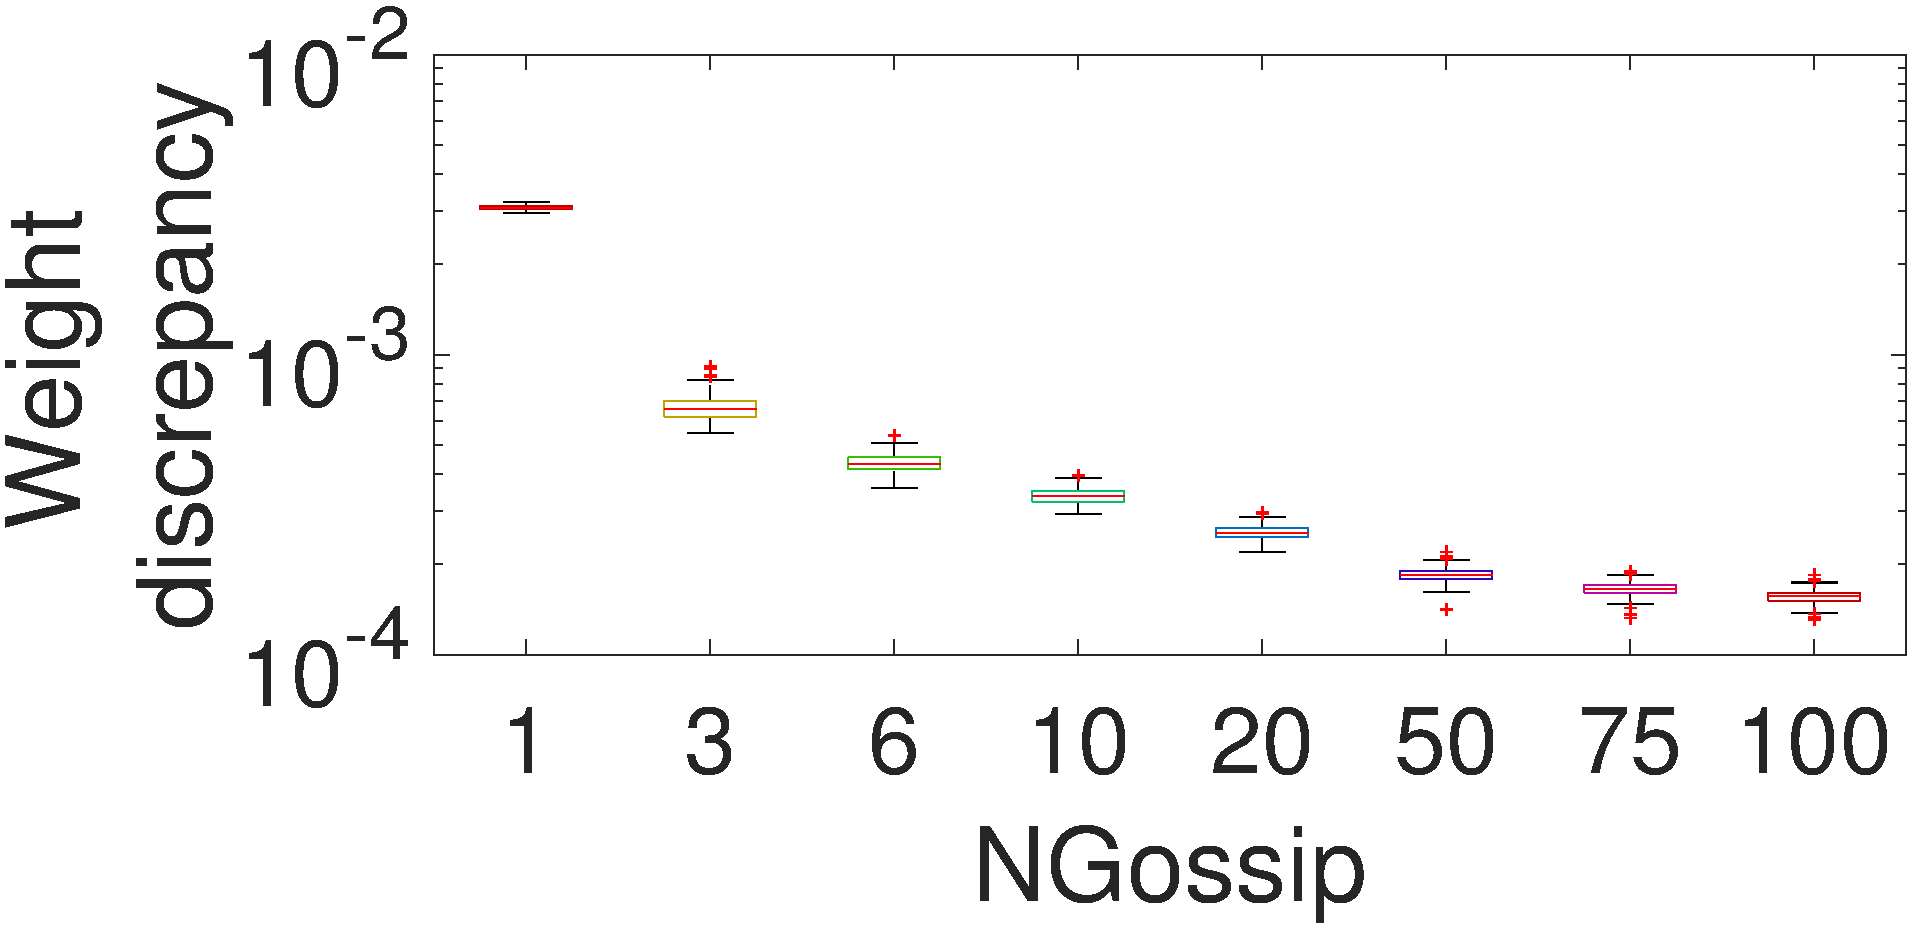
\includegraphics[width=0.6\textwidth]{Figures/boxplot_LApf_weight_discrepancy}
\caption{Boxplot of weight discrepancy with respect to $m$}
\label{fig:boxplot_LApf_weight_discrepancy}
\end{figure}

\subsection{Cluster particle filter}
The number of clusters $C$ offers a trade-off between tracking performance and computational/communication overhead. Higher number of clusters should yield better performance albeit at higher overhead. In fact, it is clear that the parameter $C$ is analogous to $m$ in LApf. Fig.~\ref{fig:results_Clusterpf} shows the tracking results. 

Again, we omit the curve for $C=1$ as the filer breaks down and yields an RMSE above 12. For $C\geq 6$, the RMSE is quite consistent for $NGossip \geq 6$. As in the case of LApf, Clusterpf is quite robust to gossiping error and yields good performance for $NGossip \geq 5$. 

As in the case of LApf, we compute and report the average weight discrepancy in Fig.~\ref{fig:boxplot_Clusterpf_weight_discrepancy}. The discrepancy is highest at $C=1$ as expected. Increasing $C$ from 6 to 75 decreases the approximation error by no more than half at the cost of a tenfold increase in communication overhead. 

\begin{figure}
\centering
\begin{subfigure}[RMSE]
{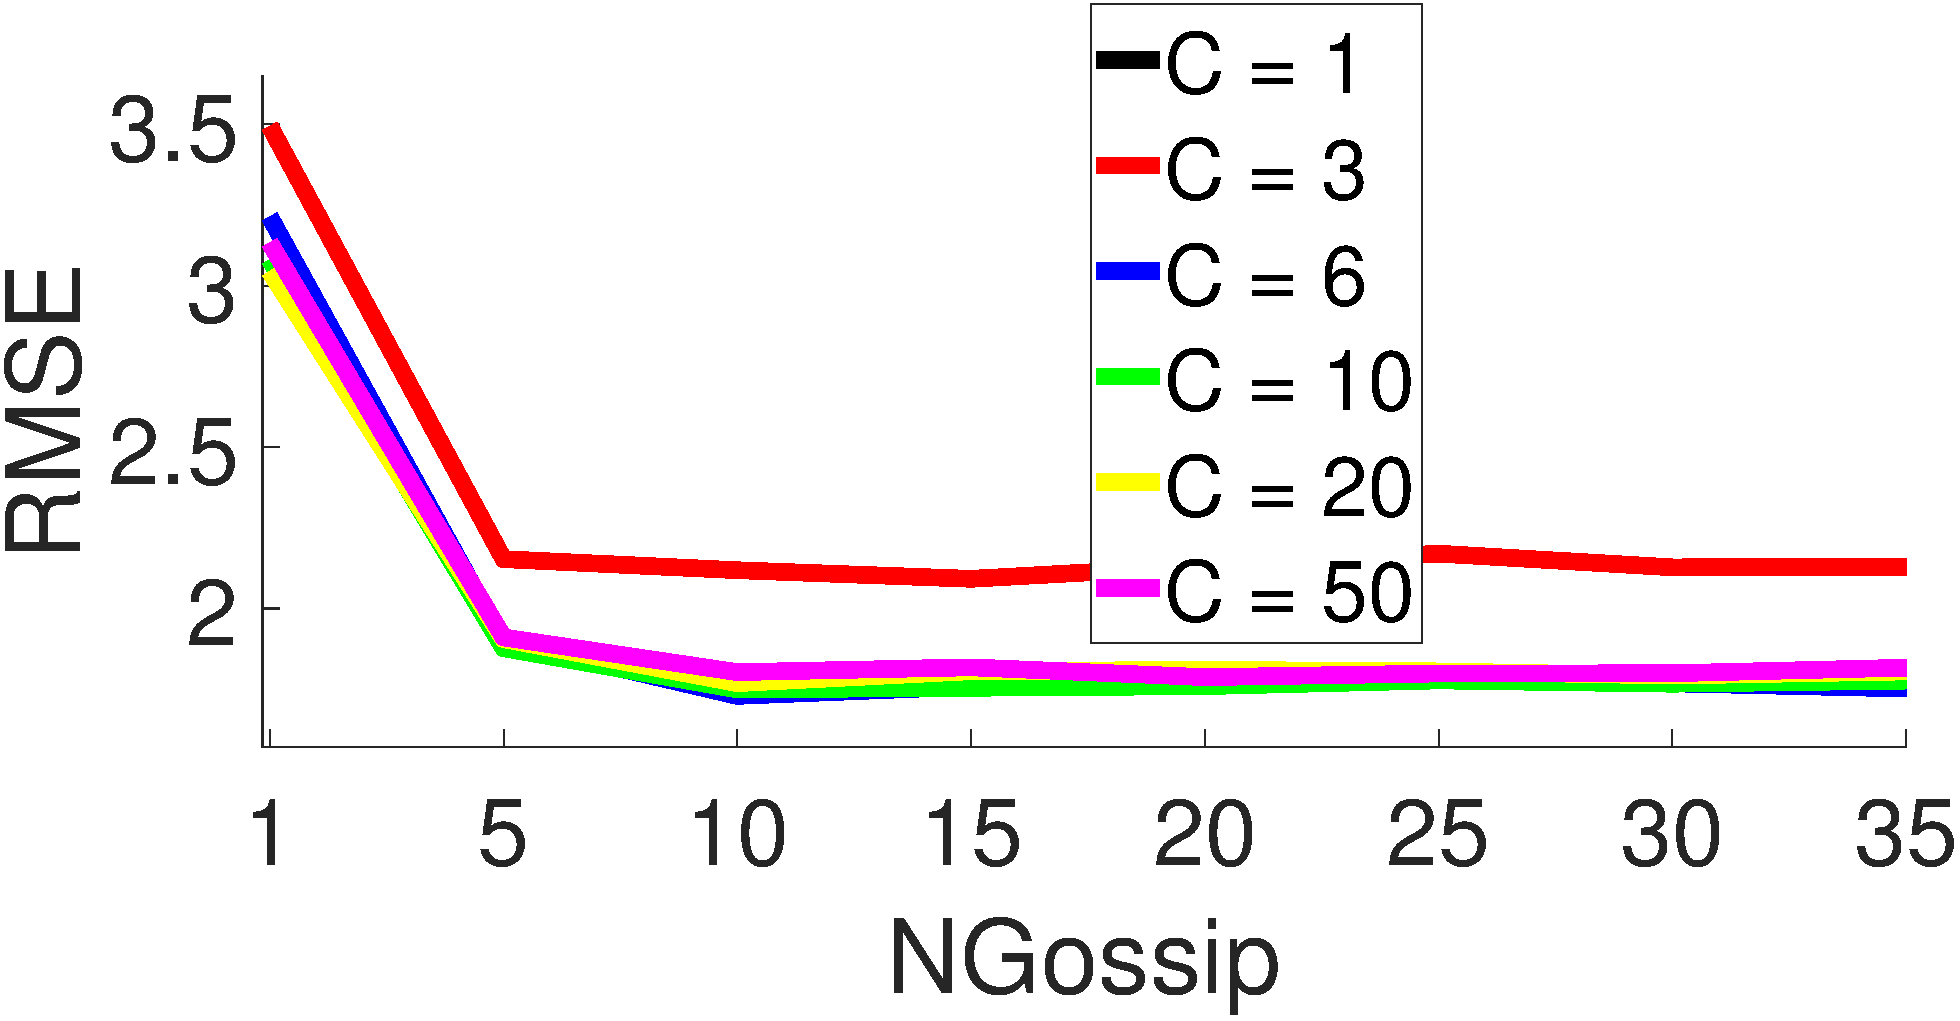
\includegraphics[width=0.49\textwidth]{Figures/curve_Clusterpf_RMSE}}
\end{subfigure}
%\begin{subfigure}[total runtime]
%{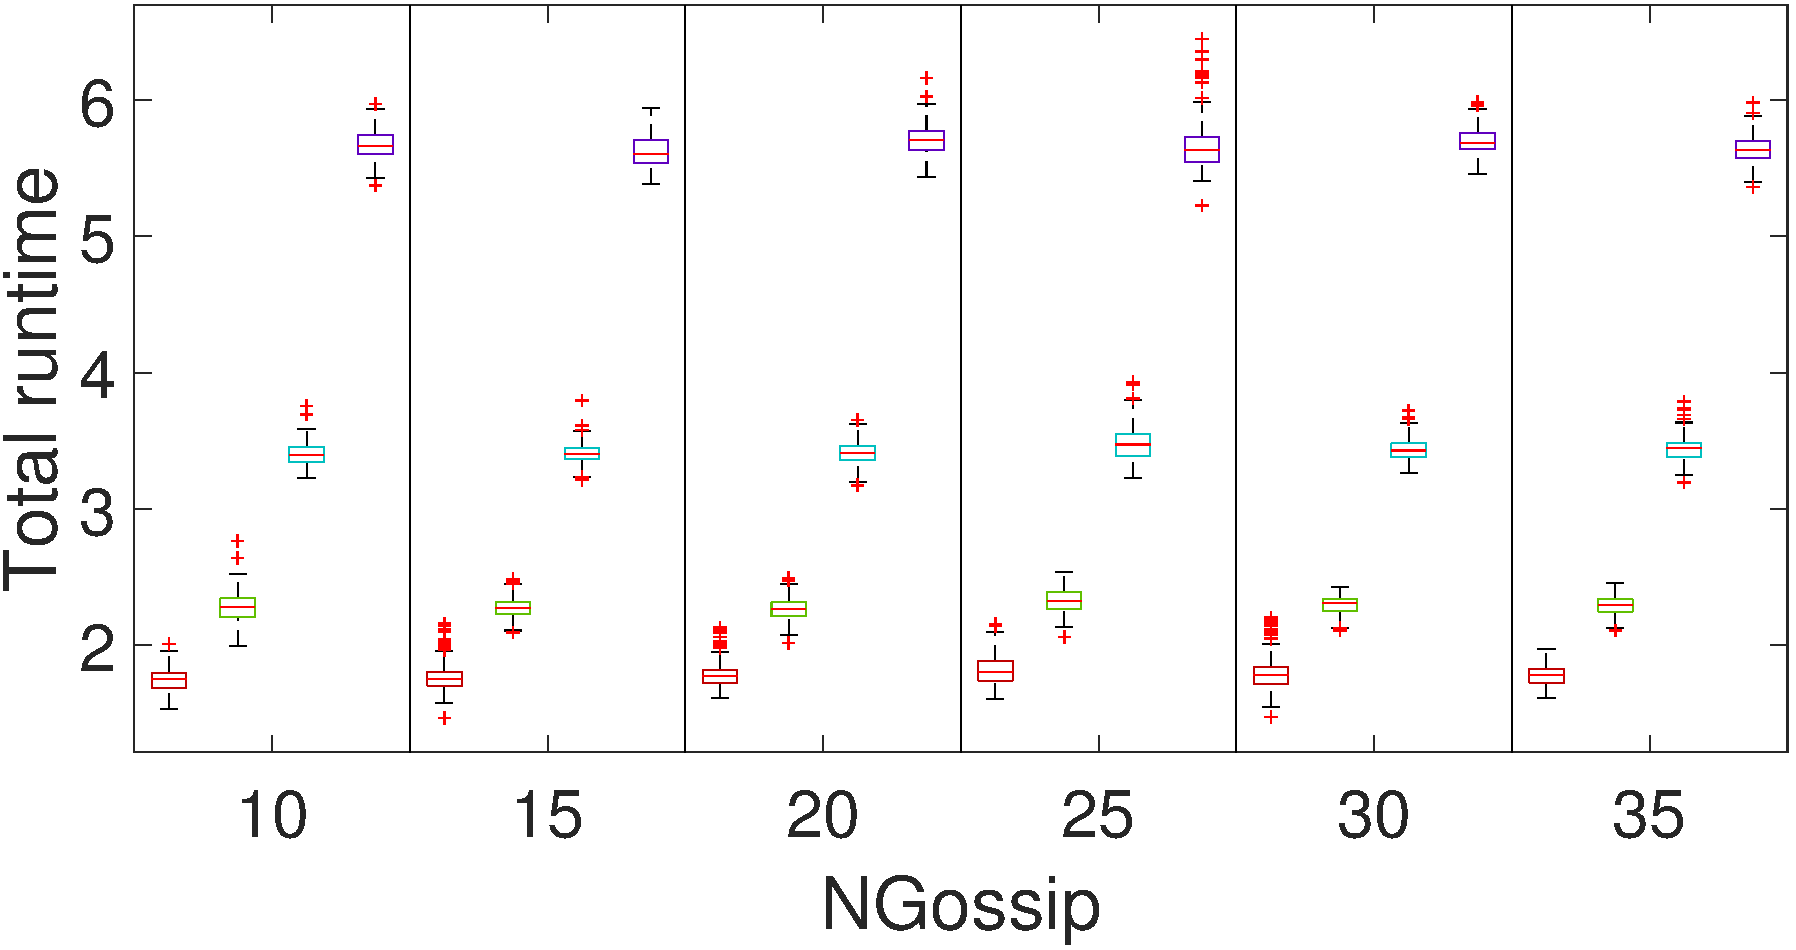
\includegraphics[width=0.65\textwidth]{Figures/boxplot_Clusterpf_time}}
%\end{subfigure}
\begin{subfigure}[AER]
{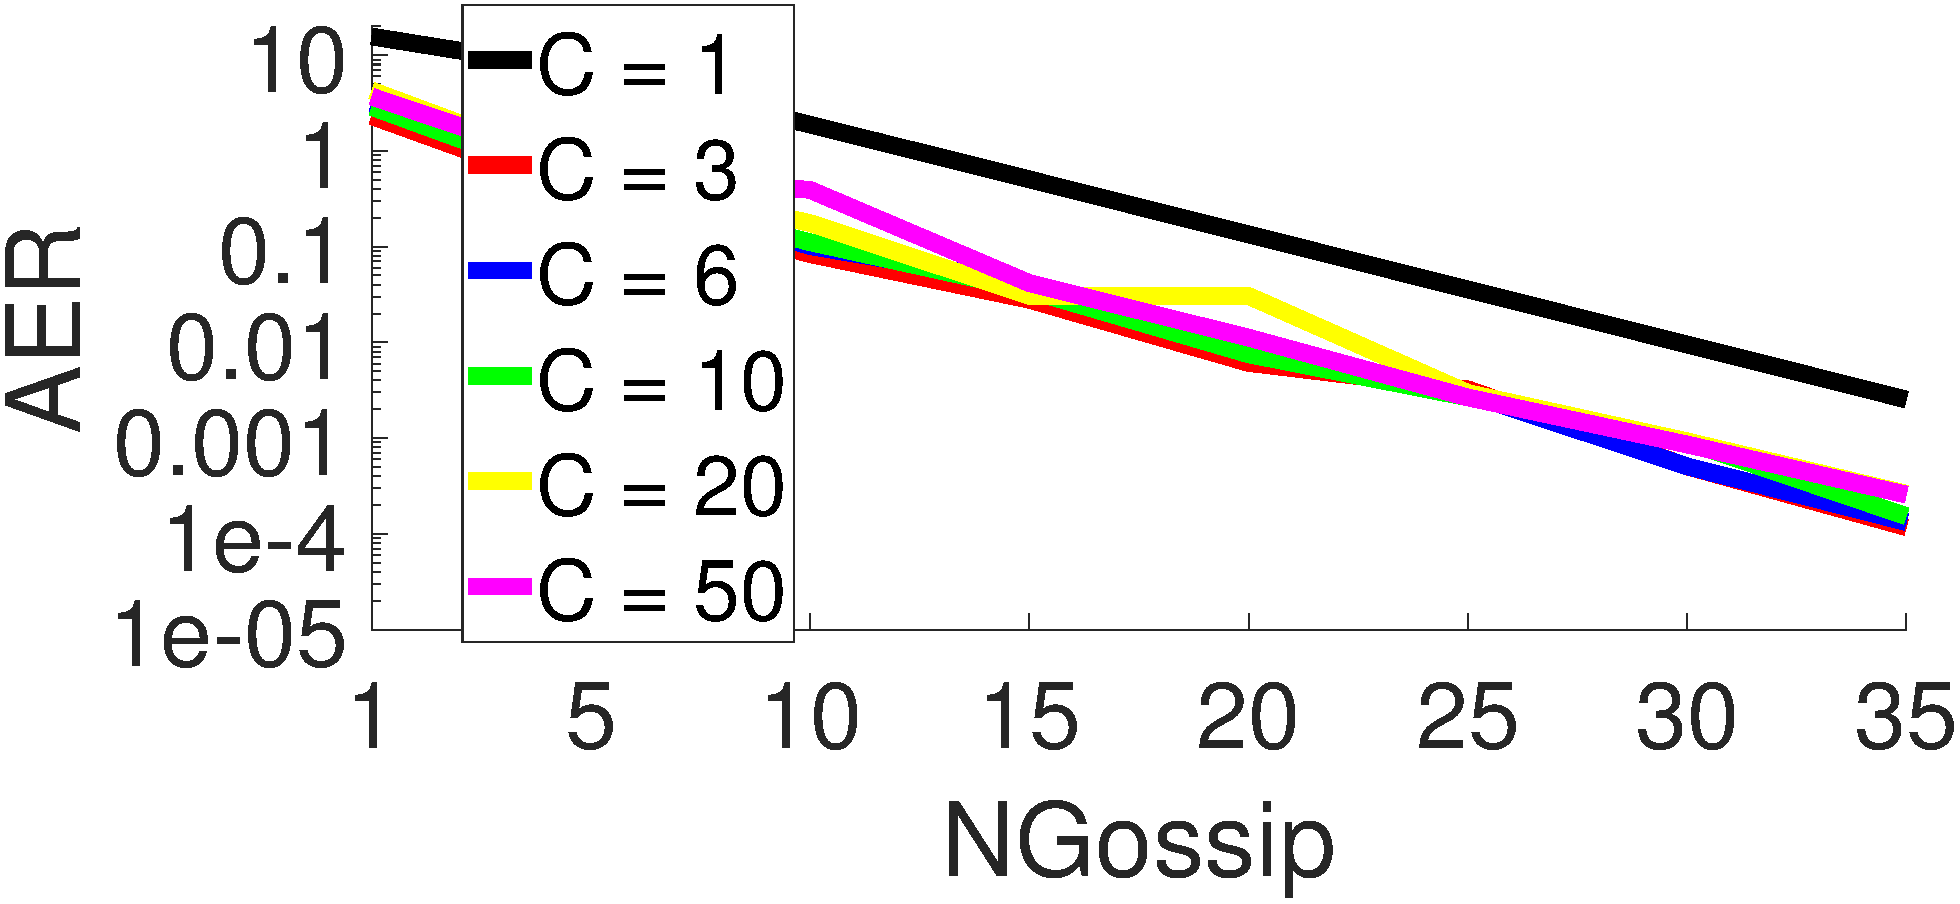
\includegraphics[width=0.49\textwidth]{Figures/curve_Clusterpf_AER}}
\end{subfigure}
\caption{RMSE and AER of Clusterpf with respect to $NGossip$ for $N=500$ and different values of $C$. All data points are averaged over 50 time steps and 200 Monte Carlo trials.}
\label{fig:results_Clusterpf}
\end{figure}

\begin{figure}
\centering
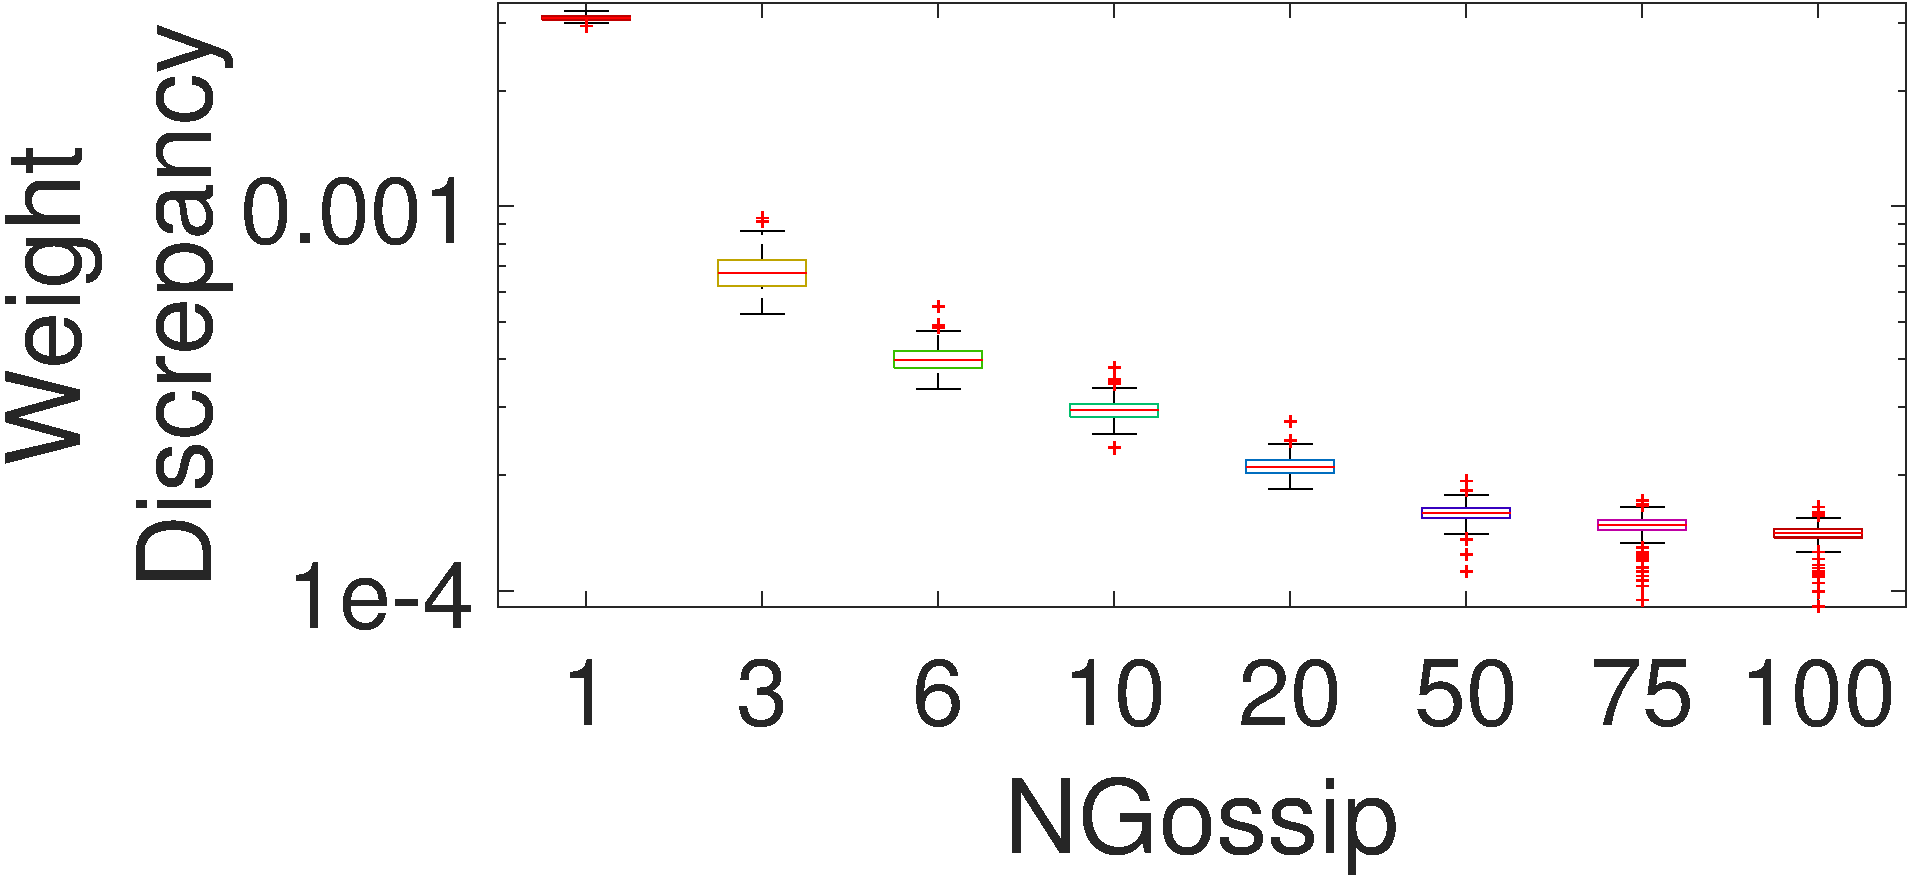
\includegraphics[width=0.6\textwidth]{Figures/boxplot_Clusterpf_weight_discrepancy}
\caption{Boxplot of weight discrepancy with respect to $C$}
\label{fig:boxplot_Clusterpf_weight_discrepancy}
\end{figure}

\subsection{Performance comparison between filters}
In this section, we compare the four filters against each other. We also include a centralized bootstrap particle filter as baseline. All four filters contain a number of algorithm-specific parameters that affect their performance, and tweaking each parameter for optimal performance is difficult. Instead we adjust the parameters such that all algorithms have the same communication overhead at each time step and compare their performance in terms of RMSE and total runtime. We consider three difficult test tracks shown in Fig.~\ref{fig:test_tracks}. 

\begin{figure}
\centering
\begin{subfigure}[Track 1]
{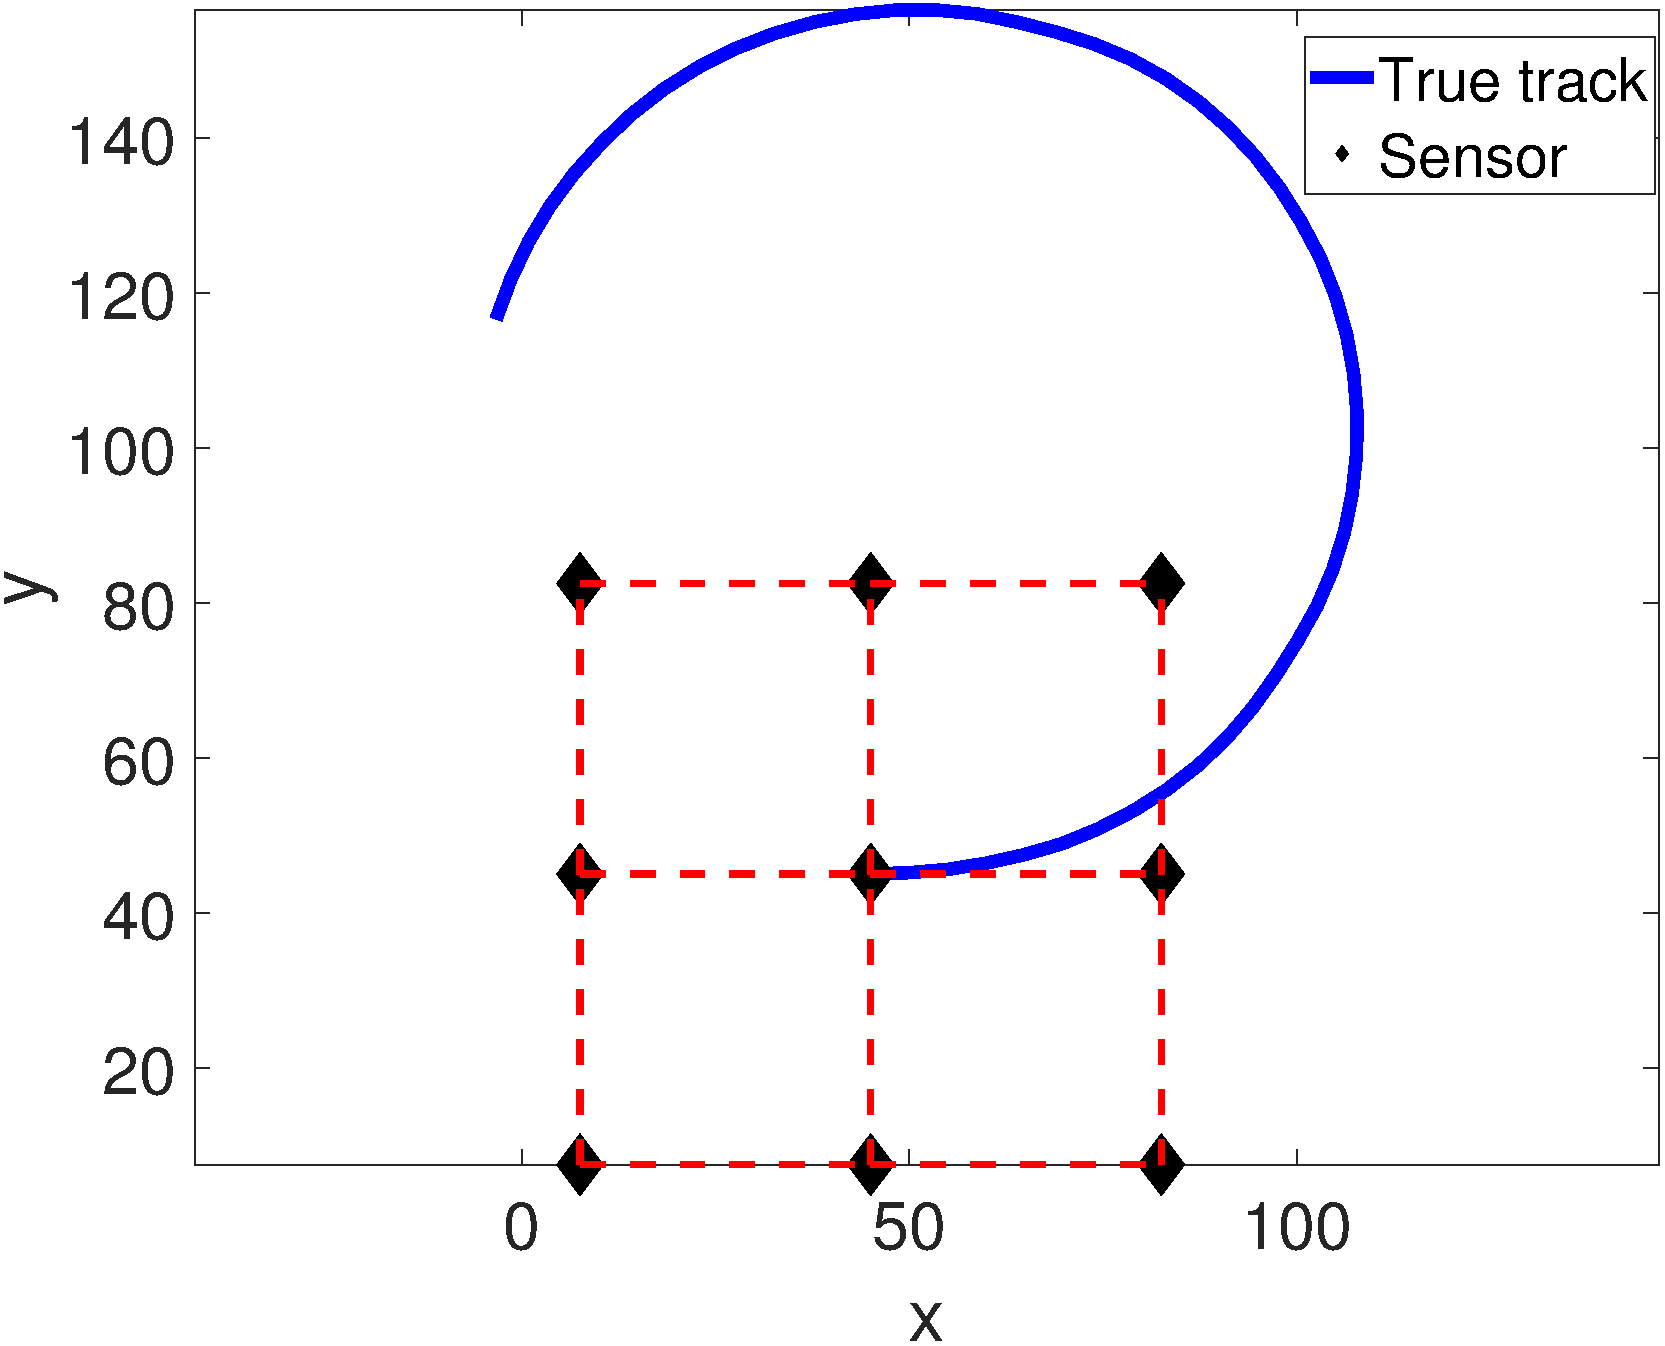
\includegraphics[width=0.32\textwidth]{Figures/track}}
\end{subfigure}
\begin{subfigure}[Track 2]
{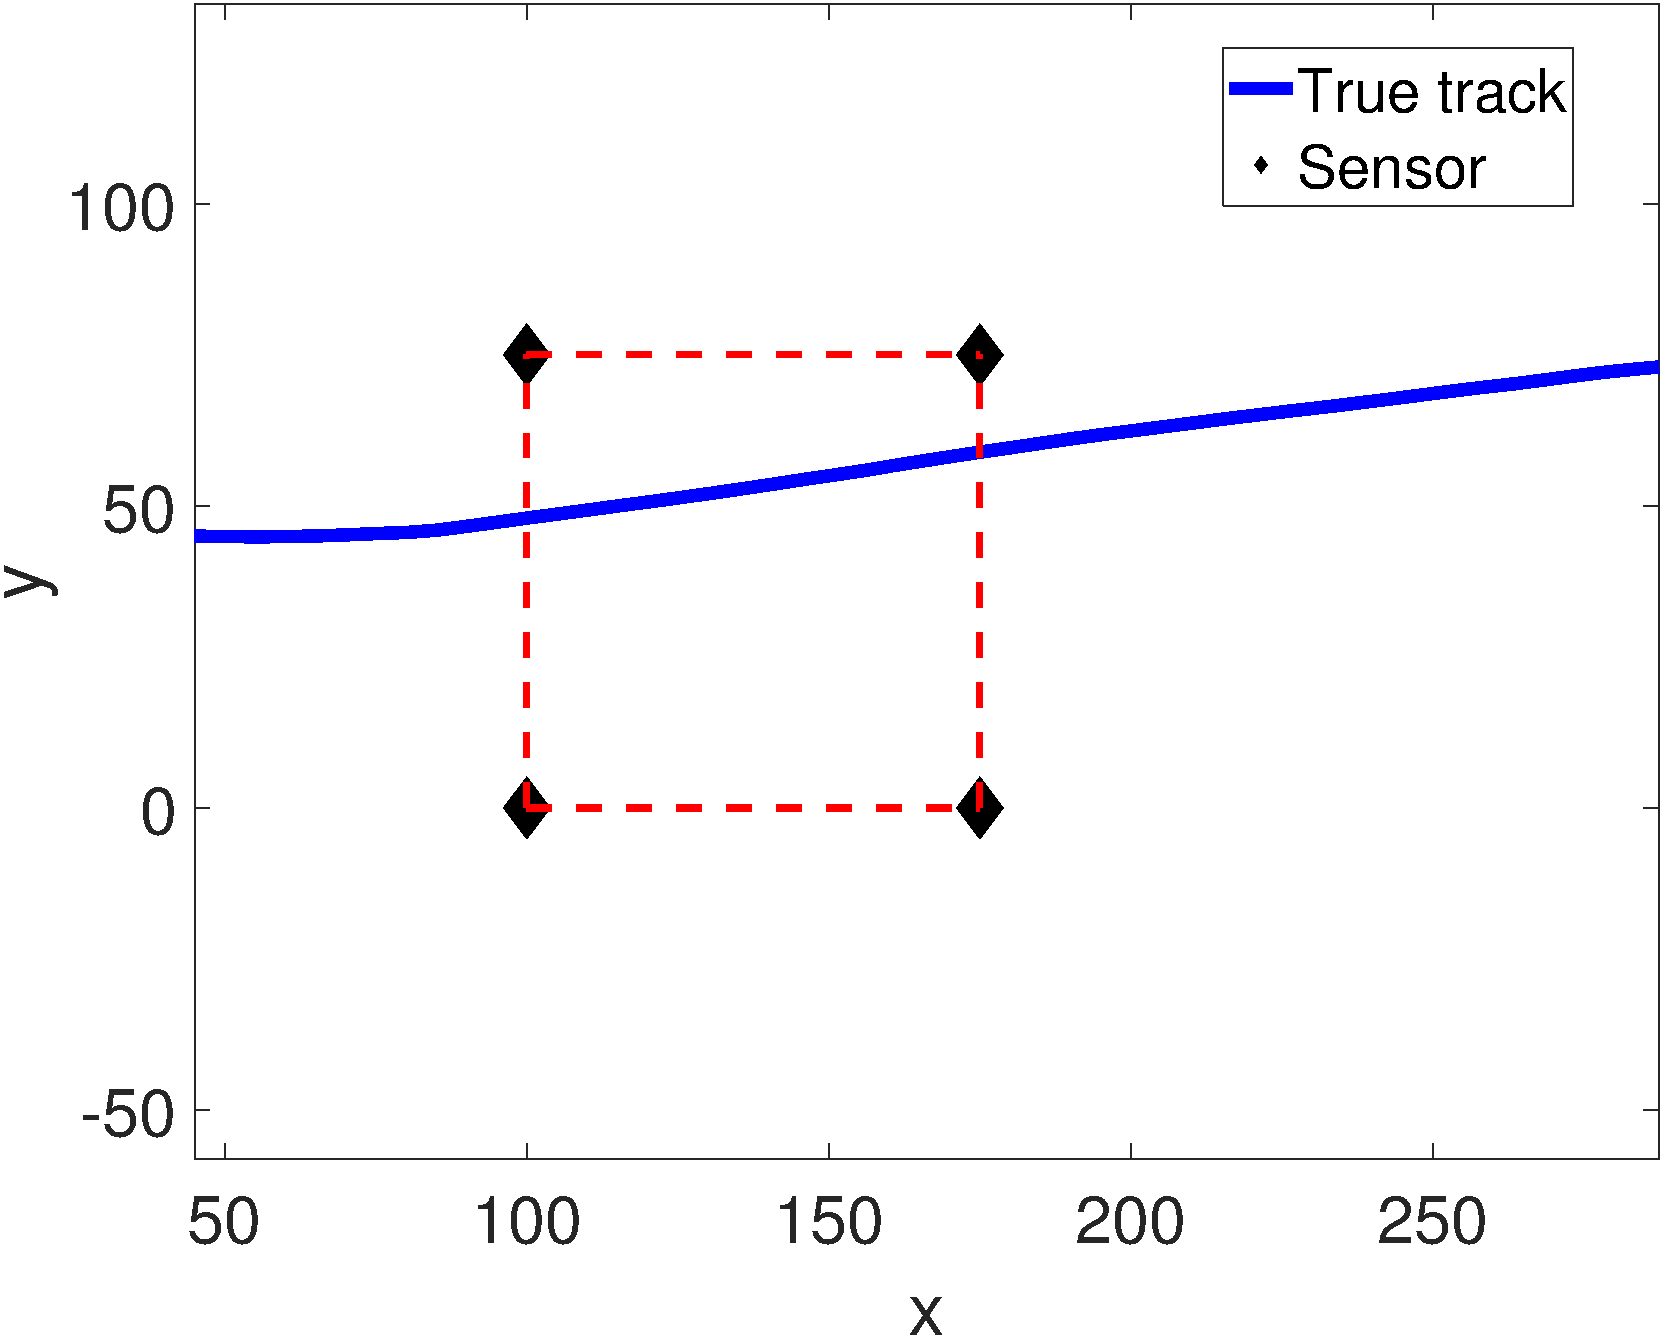
\includegraphics[width=0.32\textwidth]{Figures/track1}}
\end{subfigure}
\begin{subfigure}[Track 3]
{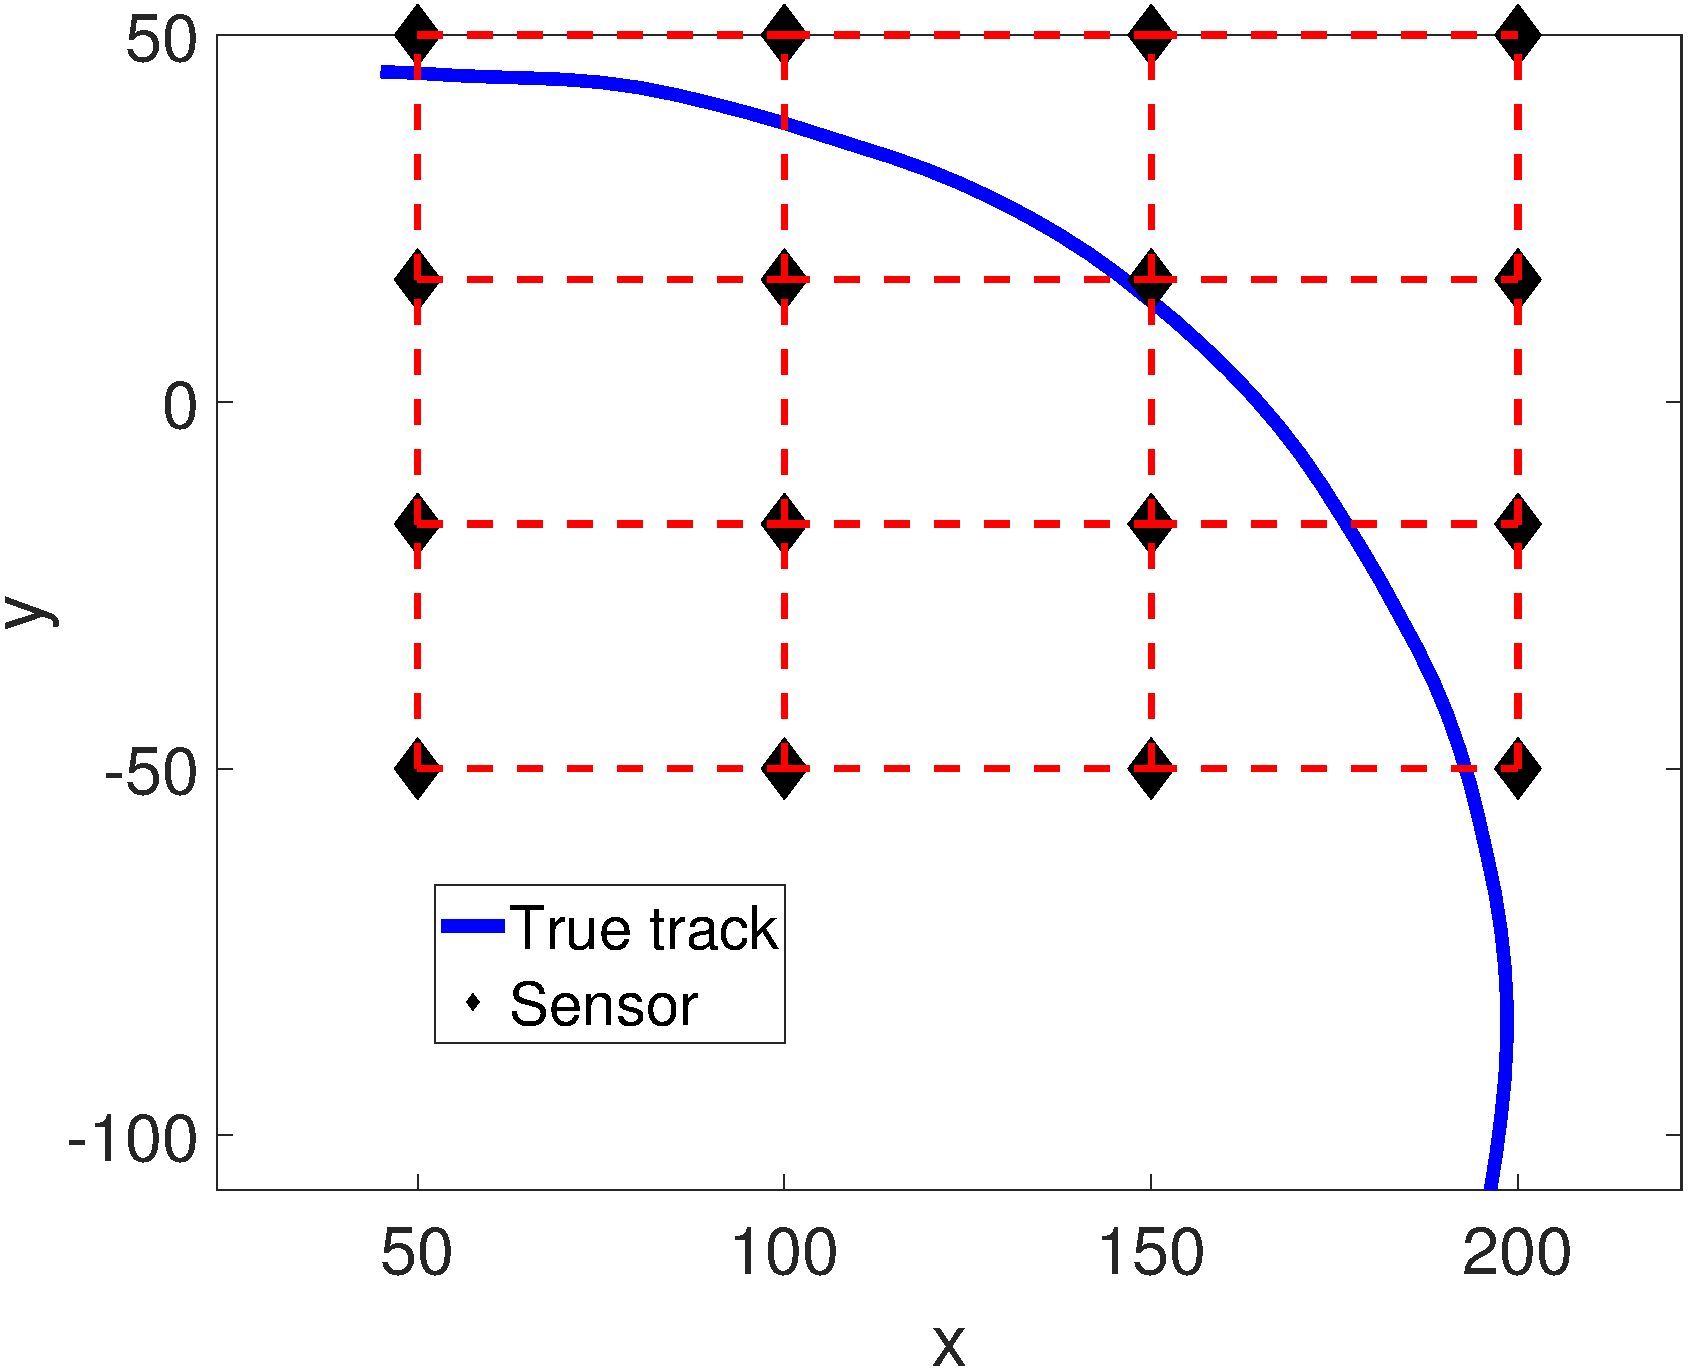
\includegraphics[width=0.32\textwidth]{Figures/track2}}
\end{subfigure}
\caption{Target tracks (blue curve) and sensor positions (black diamond). Sensors connected by red dashed lines are within broadcast range of each other.}
\label{fig:test_tracks}
\end{figure}

Fig.~\ref{fig:Track3_results} shows the average RMSE and total runtime with respect to communication overhead per time step for all algorithms for track 1. For CSSpf and LCpf, we vary only the number of gossip iterations per time step. We run two variations of LApf and Clusterpf. In the first version, we fix $m$ and $C$, the number of scalars to aggregate per time step, and increase $NGossip$. In the second version, we fix $NGossip$ and increase $m$ and $C$ accordingly. 

The LCpf has very high RMSE until $NGossip=42$ (i.e., total overhead = 42*20 = 840). This is consistent with our previous results showing that the algorithm is very susceptible to gossiping error. The CSSpf achieves good performance for $NGossip\geq 20$ but is worse than BSpf, LApf and Clusterpf. 

Both LApf and Clusterpf yield good tracking performance on-par with centralized BSpf even at lowest communication overhead. Consider the two curves of LApf. When $m$ is fixed, the RMSE goes down as $NGossip$ goes down and remains relatively constant for $NGossip\geq 70$. This would suggest that, after 70 gossip iterations, the approximate aggregate values are sufficiently close to the true aggregate values, and that any additional gossip iteration would provide marginal if any improvement. When $NGossip$ is fixed, the RMSE decreases until $m=8$ then increases afterwards. If $m$ is too low, then we do not retain enough eigenvectors to provide an adequate encoding of the particle likelihoods. If $m$ goes up, we should obtain a better encoding of the particle likelihoods but also seem to get higher error from the distributed summation (as $NGossip$ remains constant). The same trends can be observed in the two Clusterpf curves. For both filters, there is a cut-off point after which it is more beneficial to minimize number of broadcast scalars and maximize number gossip iterations (540 for LApf and 300 for Clusterpf). 

The BSpf, CSSpf and LCpf have lowest runtime as expected. For all three algorithms, increasing $NGossip$ has negligible impact on runtime due to our implementation of the gossip algorithms. LApf has highest runtime by a large margin. Varying either $NGossip$ or $m$ has no significant impact on runtime since the majority of computation overhead is attributed to eigenvalue decomposition which depends only on the number of particles. The Clusterpf also has rather high runtime. When $C$ increases, there is higher computational overhead for particle clustering and the runtime increases linearly as expected.  

\begin{figure}
\centering
\begin{subfigure}[RMSE]
{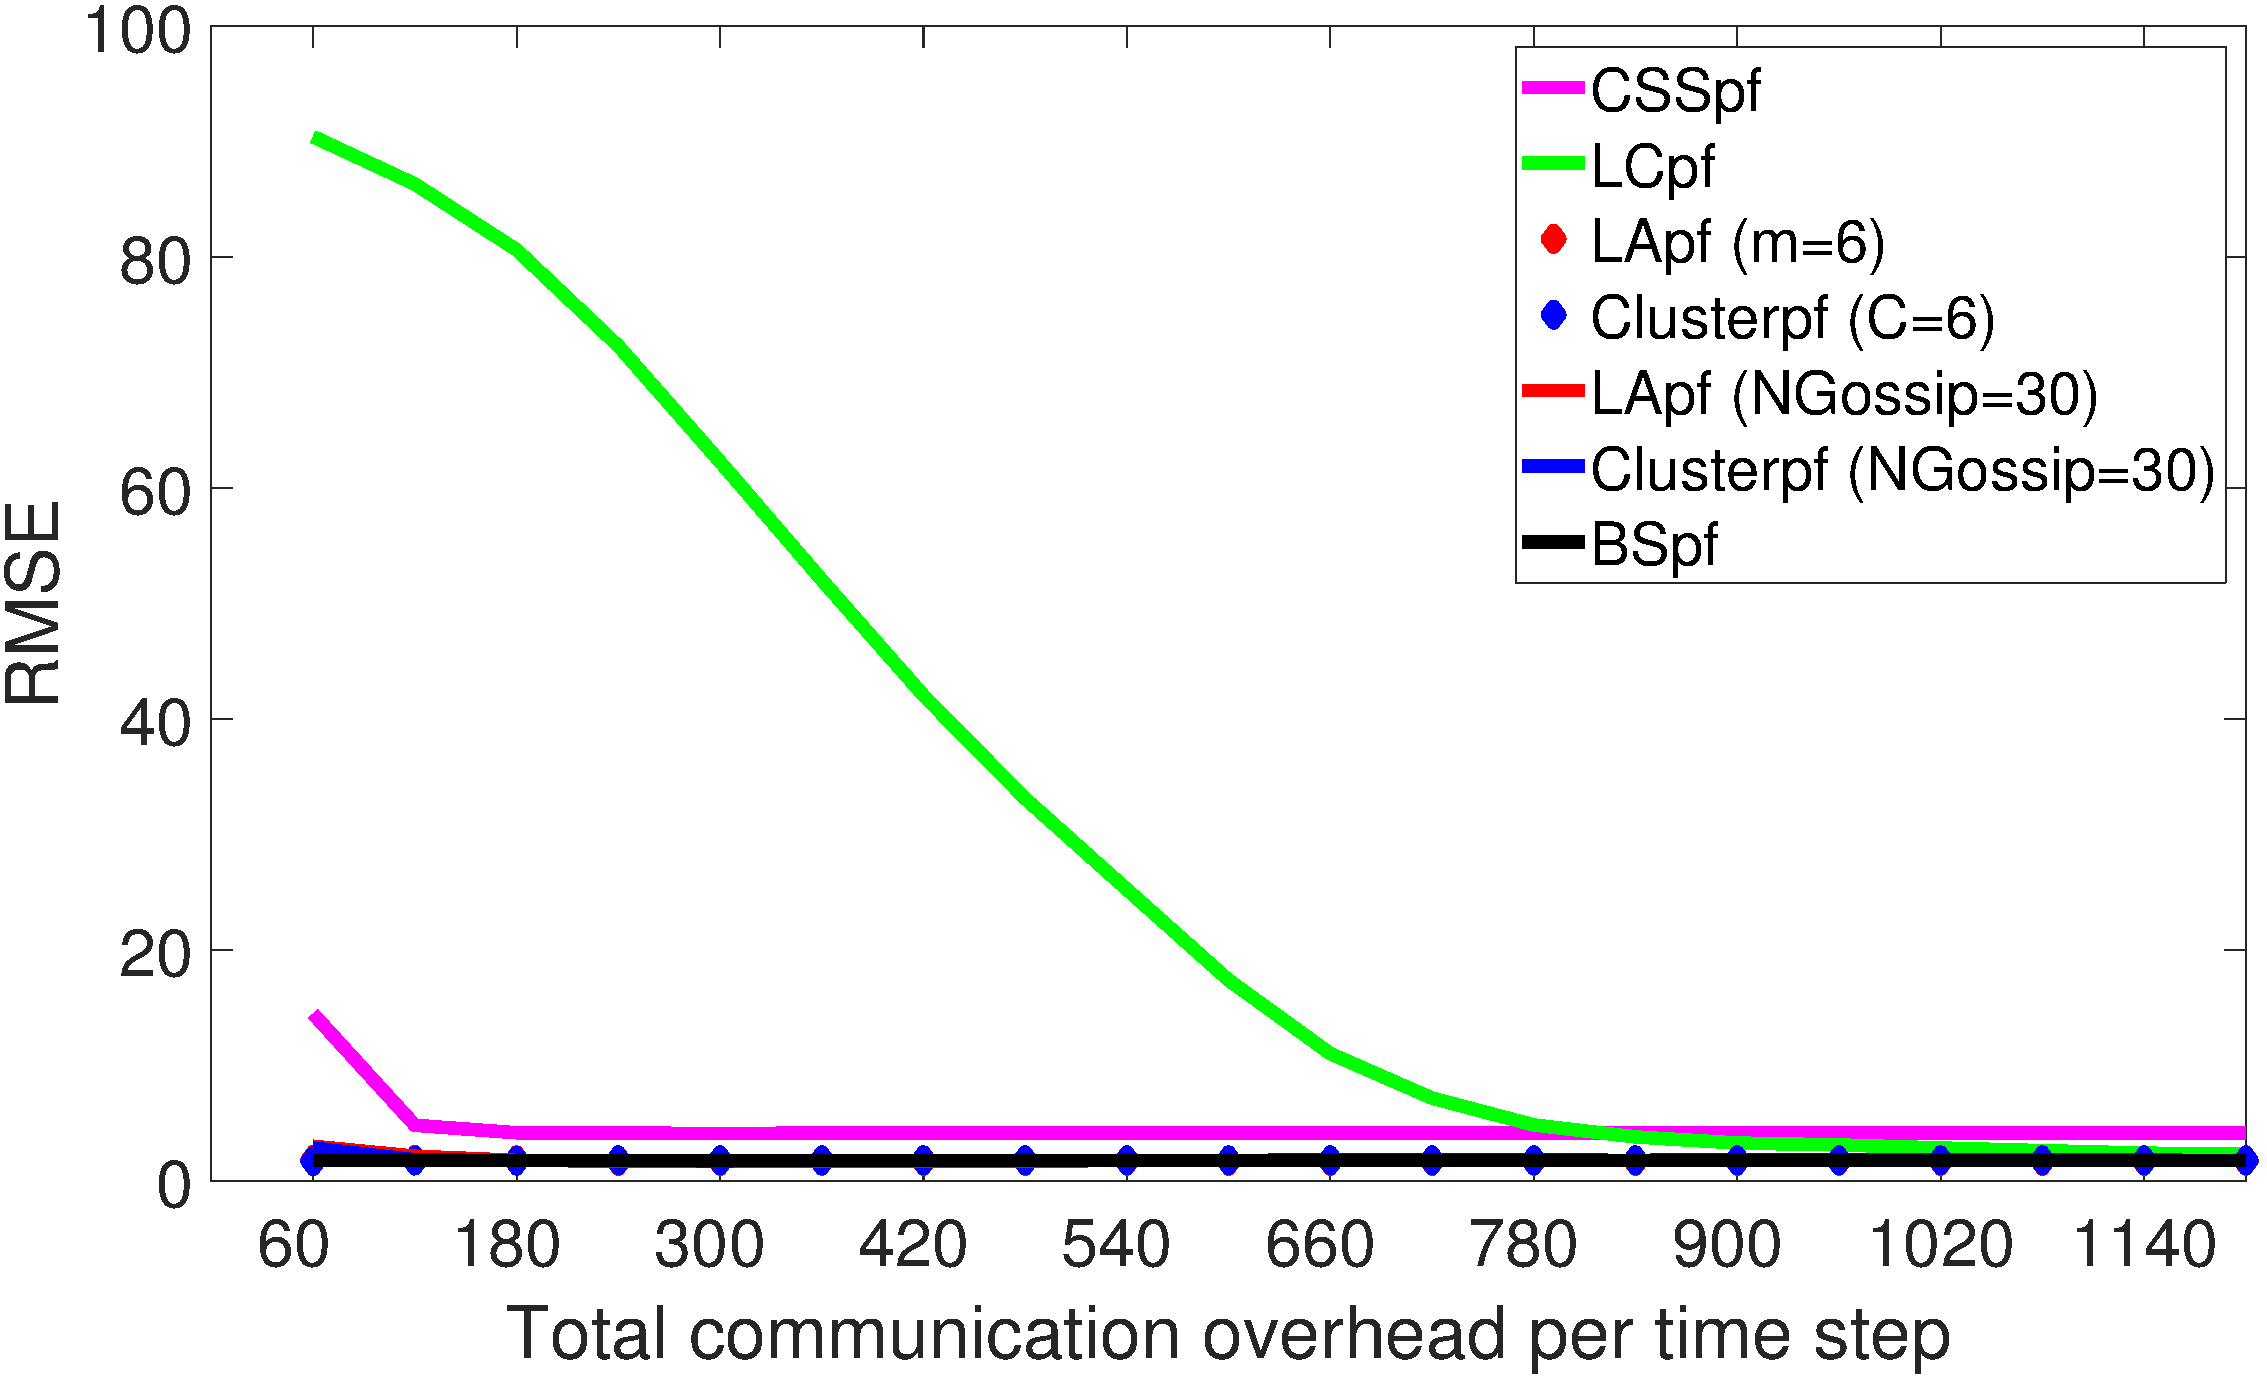
\includegraphics[width=0.65\textwidth]{Figures/Track3_RMSE}}
\end{subfigure}
\begin{subfigure}[RMSE]
{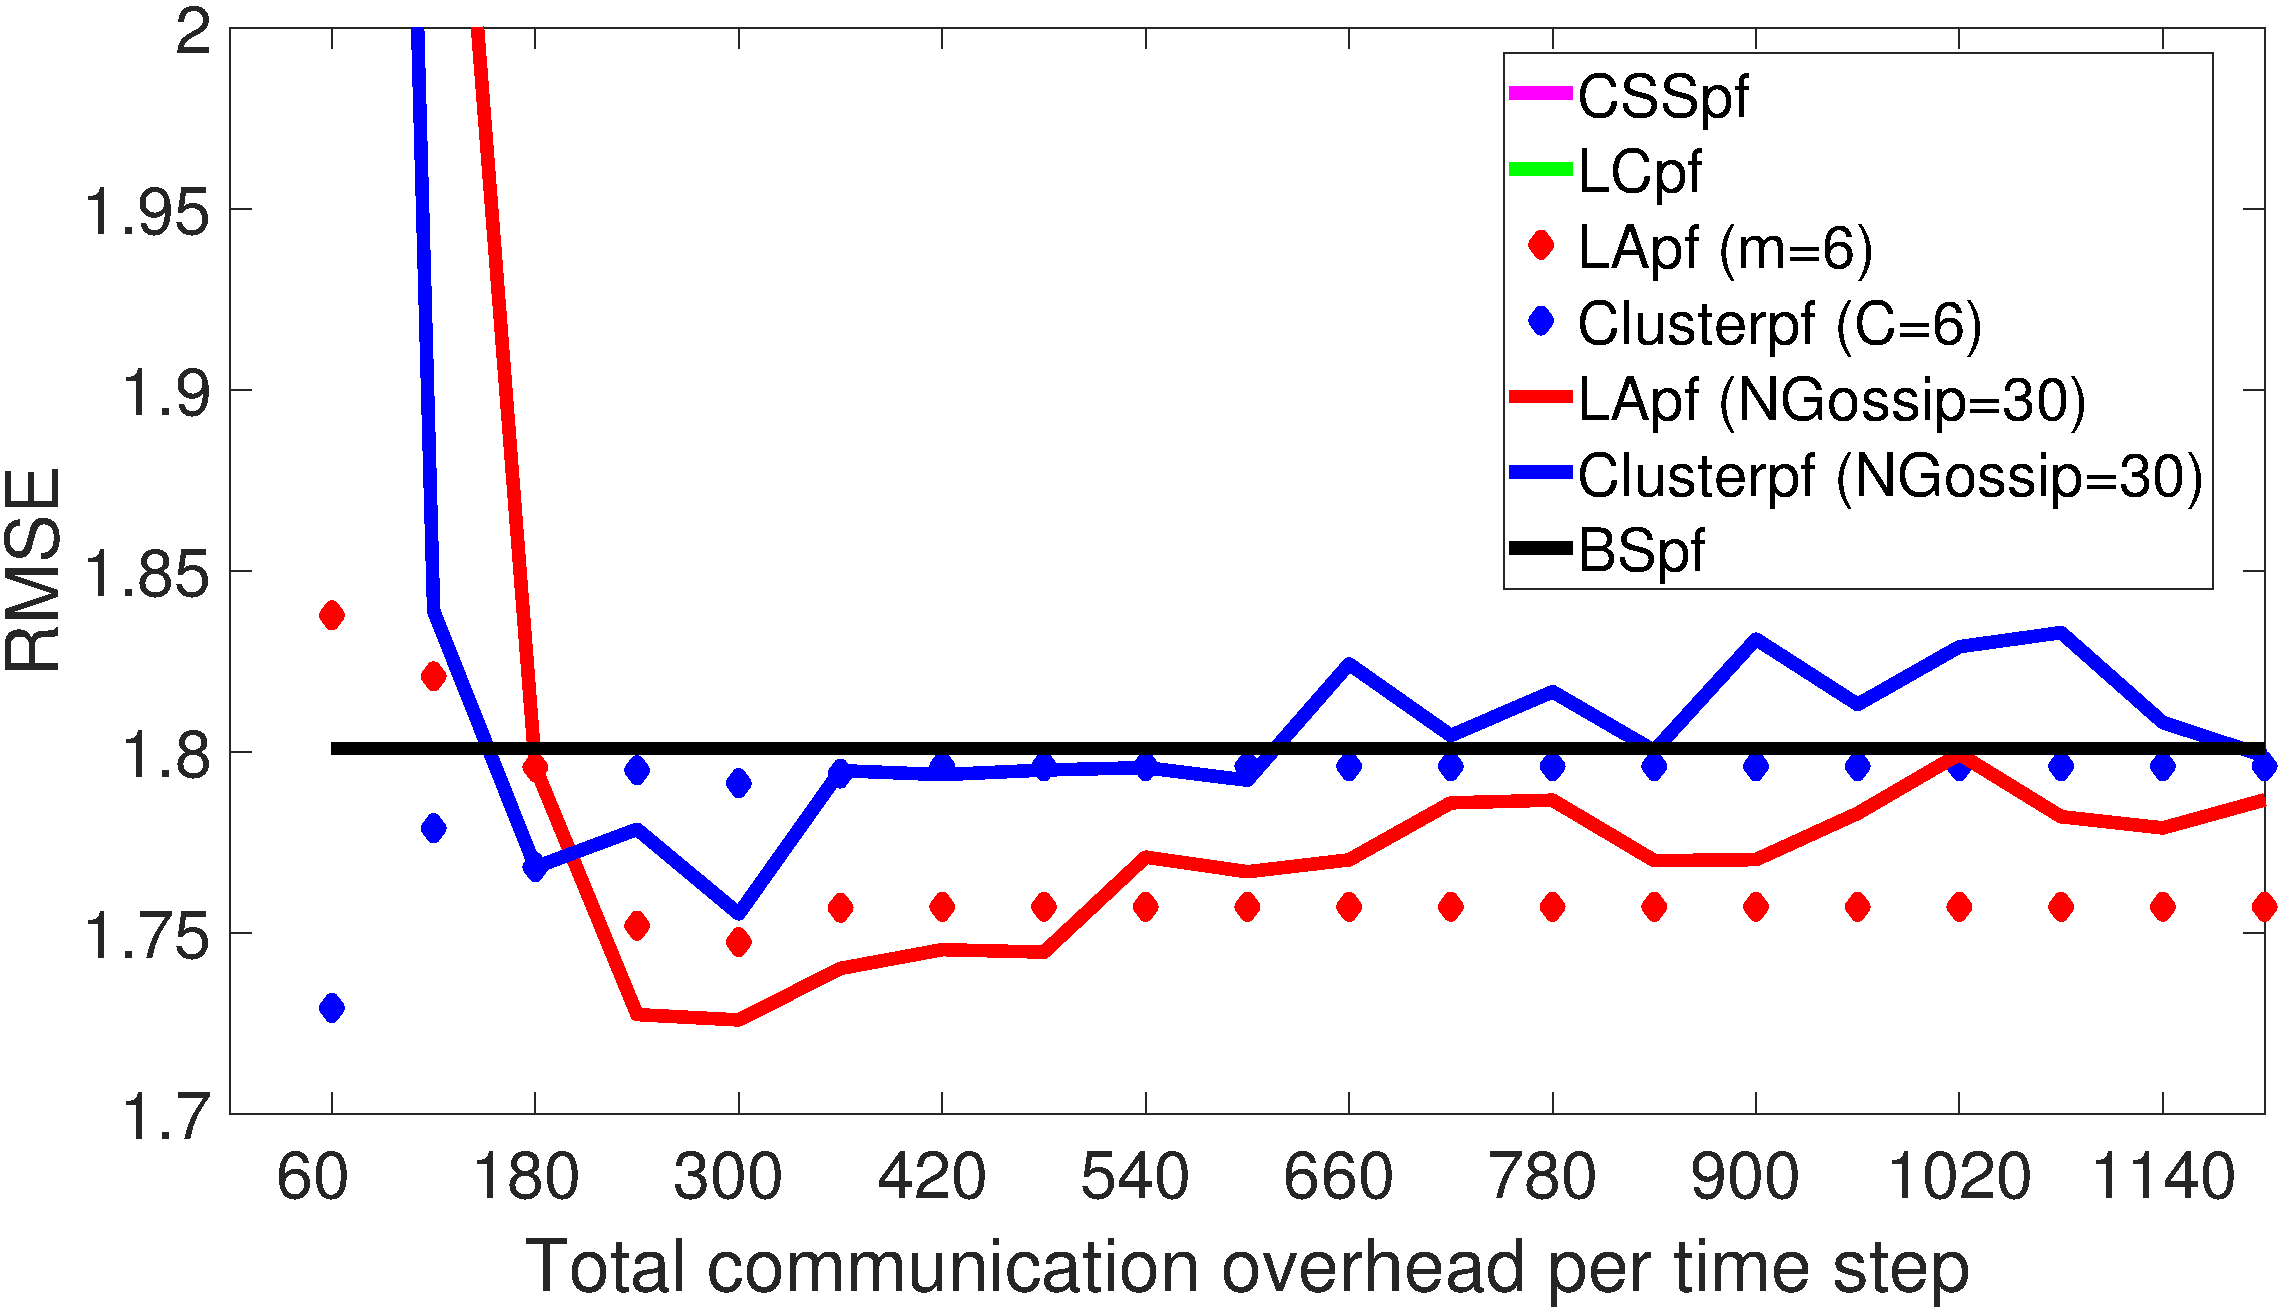
\includegraphics[width=0.65\textwidth]{Figures/Track3_RMSE_focus}}
\end{subfigure}
\begin{subfigure}[total runtime]
{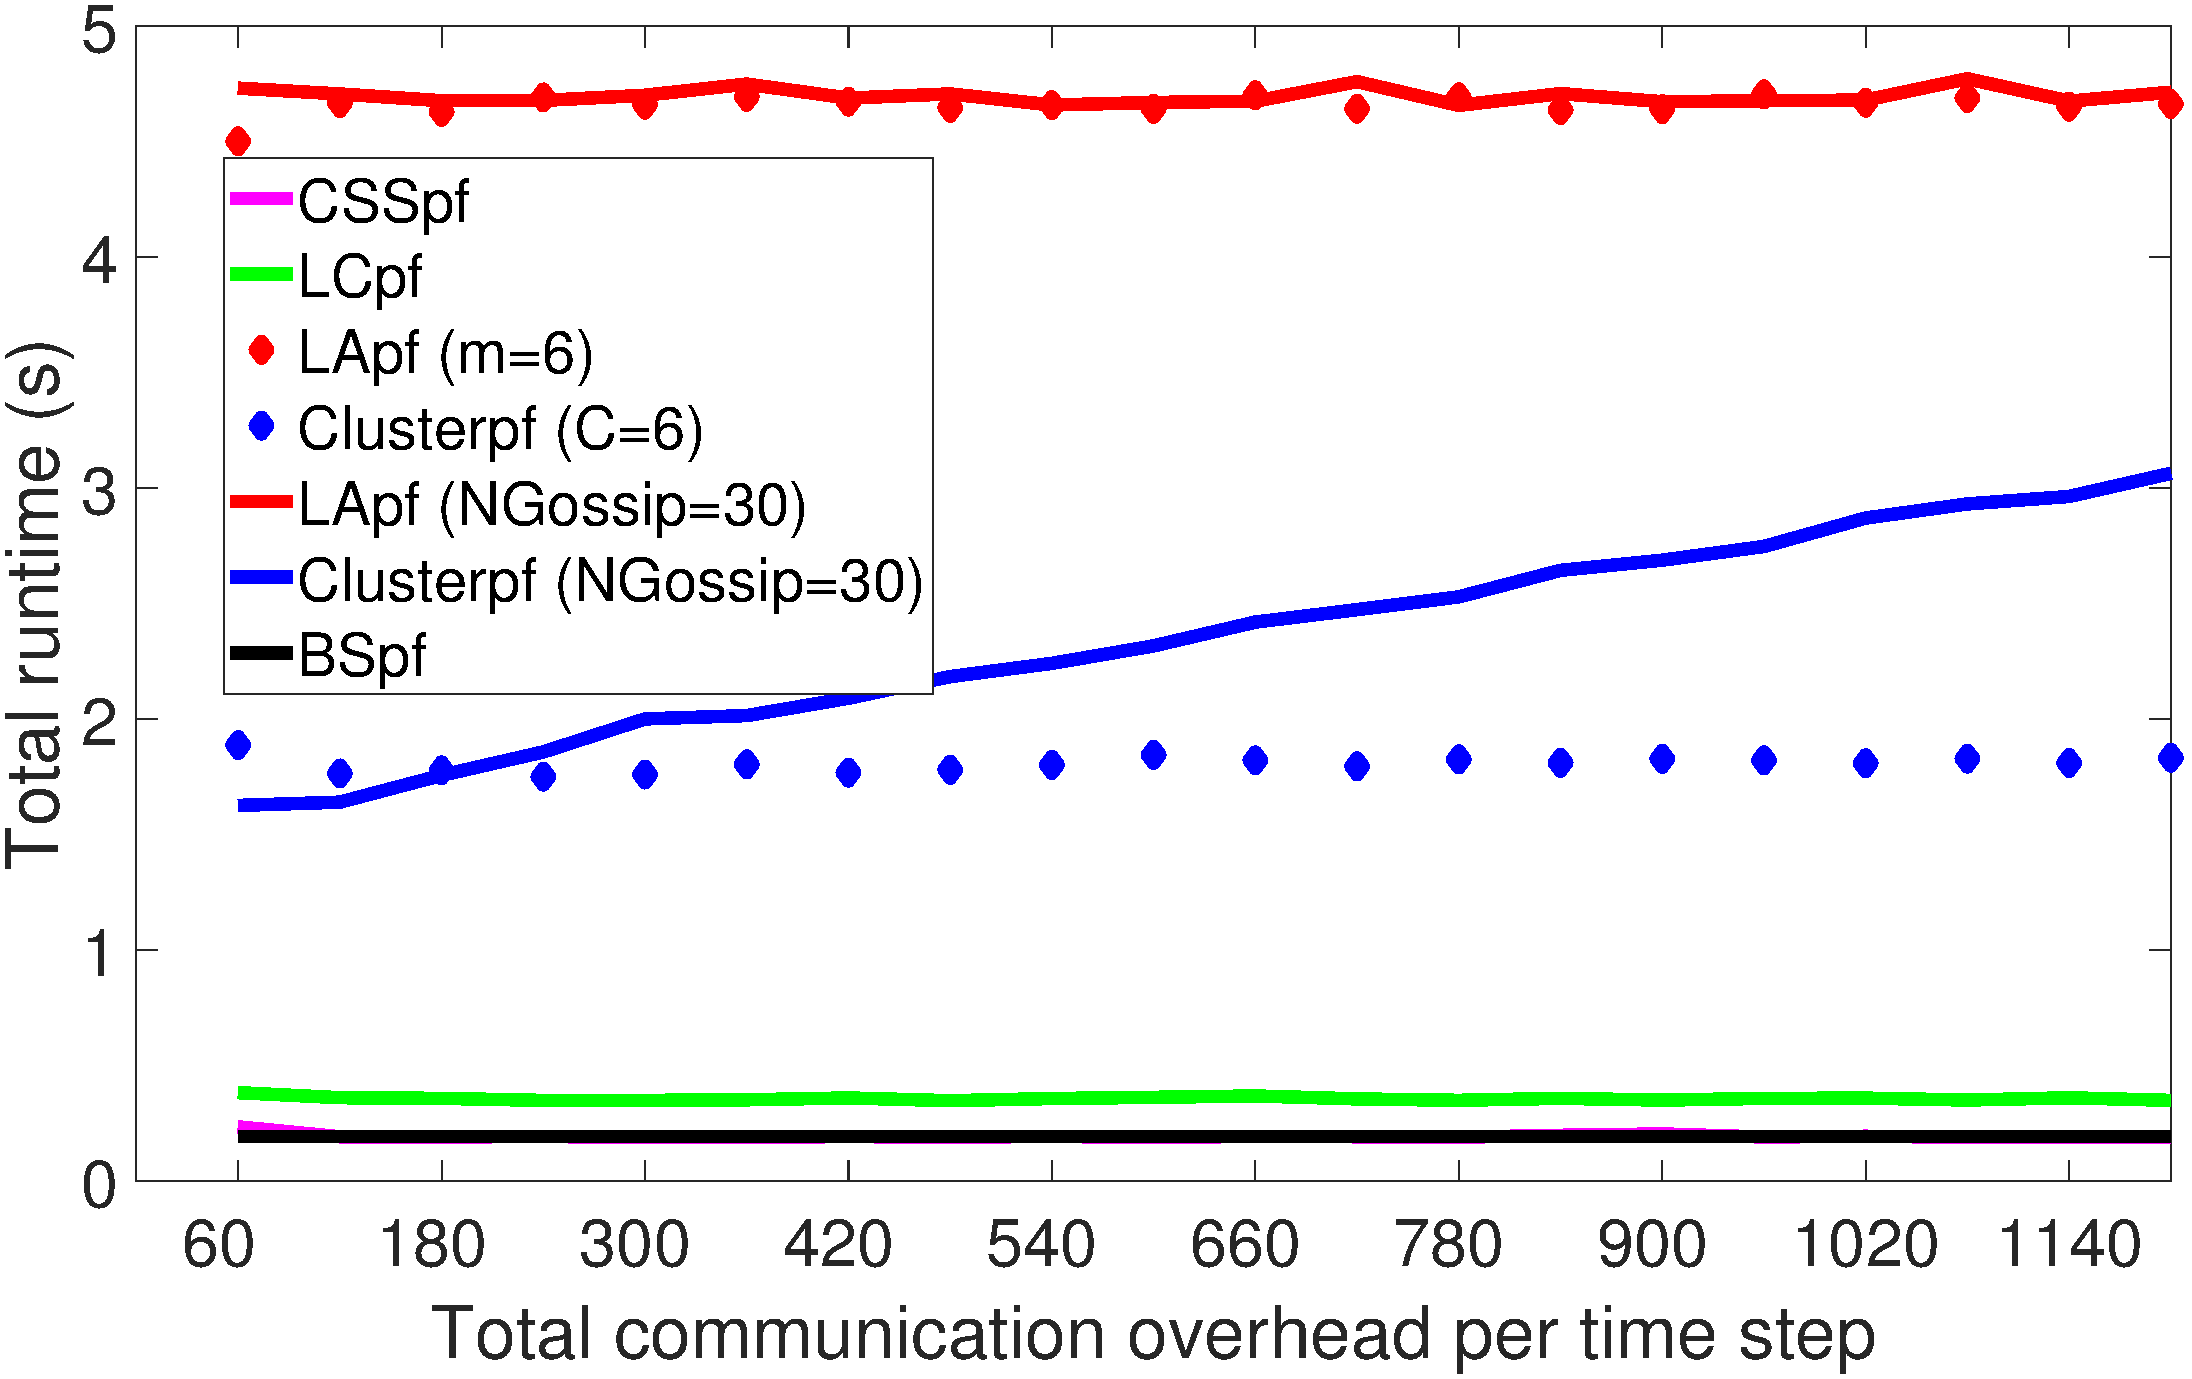
\includegraphics[width=0.65\textwidth]{Figures/Track3_runtime}}
\end{subfigure}
\caption{Average RMSE and runtime with respect to total communication overhead per time step for track 1 ($N=500$, 200 Monte Carlo trials). The subfig b) provides a zoomed view of RMSE curves.}
\label{fig:Track3_results}
\end{figure}

Fig.~\ref{fig:Track1_results} shows the tracking results for track 2. The runtime display identical trends as in the first test track so we focus our analysis on RMSE only. The CSSpf has surprisingly the best performance in this case followed by BSpf. The RMSE of LApf and Clusterpf are fairly constant when $m$ and $C$ are fixed. Since this track contains fewer sensors than track 1, fewer ($\ll 30$) gossip iterations should be required for convergence so increasing $NGossip$ would have negligible benefit. On the other hand, increasing $m$ and $C$ does reduce the RMSE of LApf and Clutterpf up till $m=10, C=10$ and yields better performance compared to the two curves with fixed $m$ and $C$. Finally, LCpf has the worst performance by far. Nonetheless, if we compare the performance of LCpf in the two test tracks, the filter only requires half the total communication overhead to achieve adequate tracking performance in track 2. 

\begin{figure}
\centering
\begin{subfigure}[RMSE]
{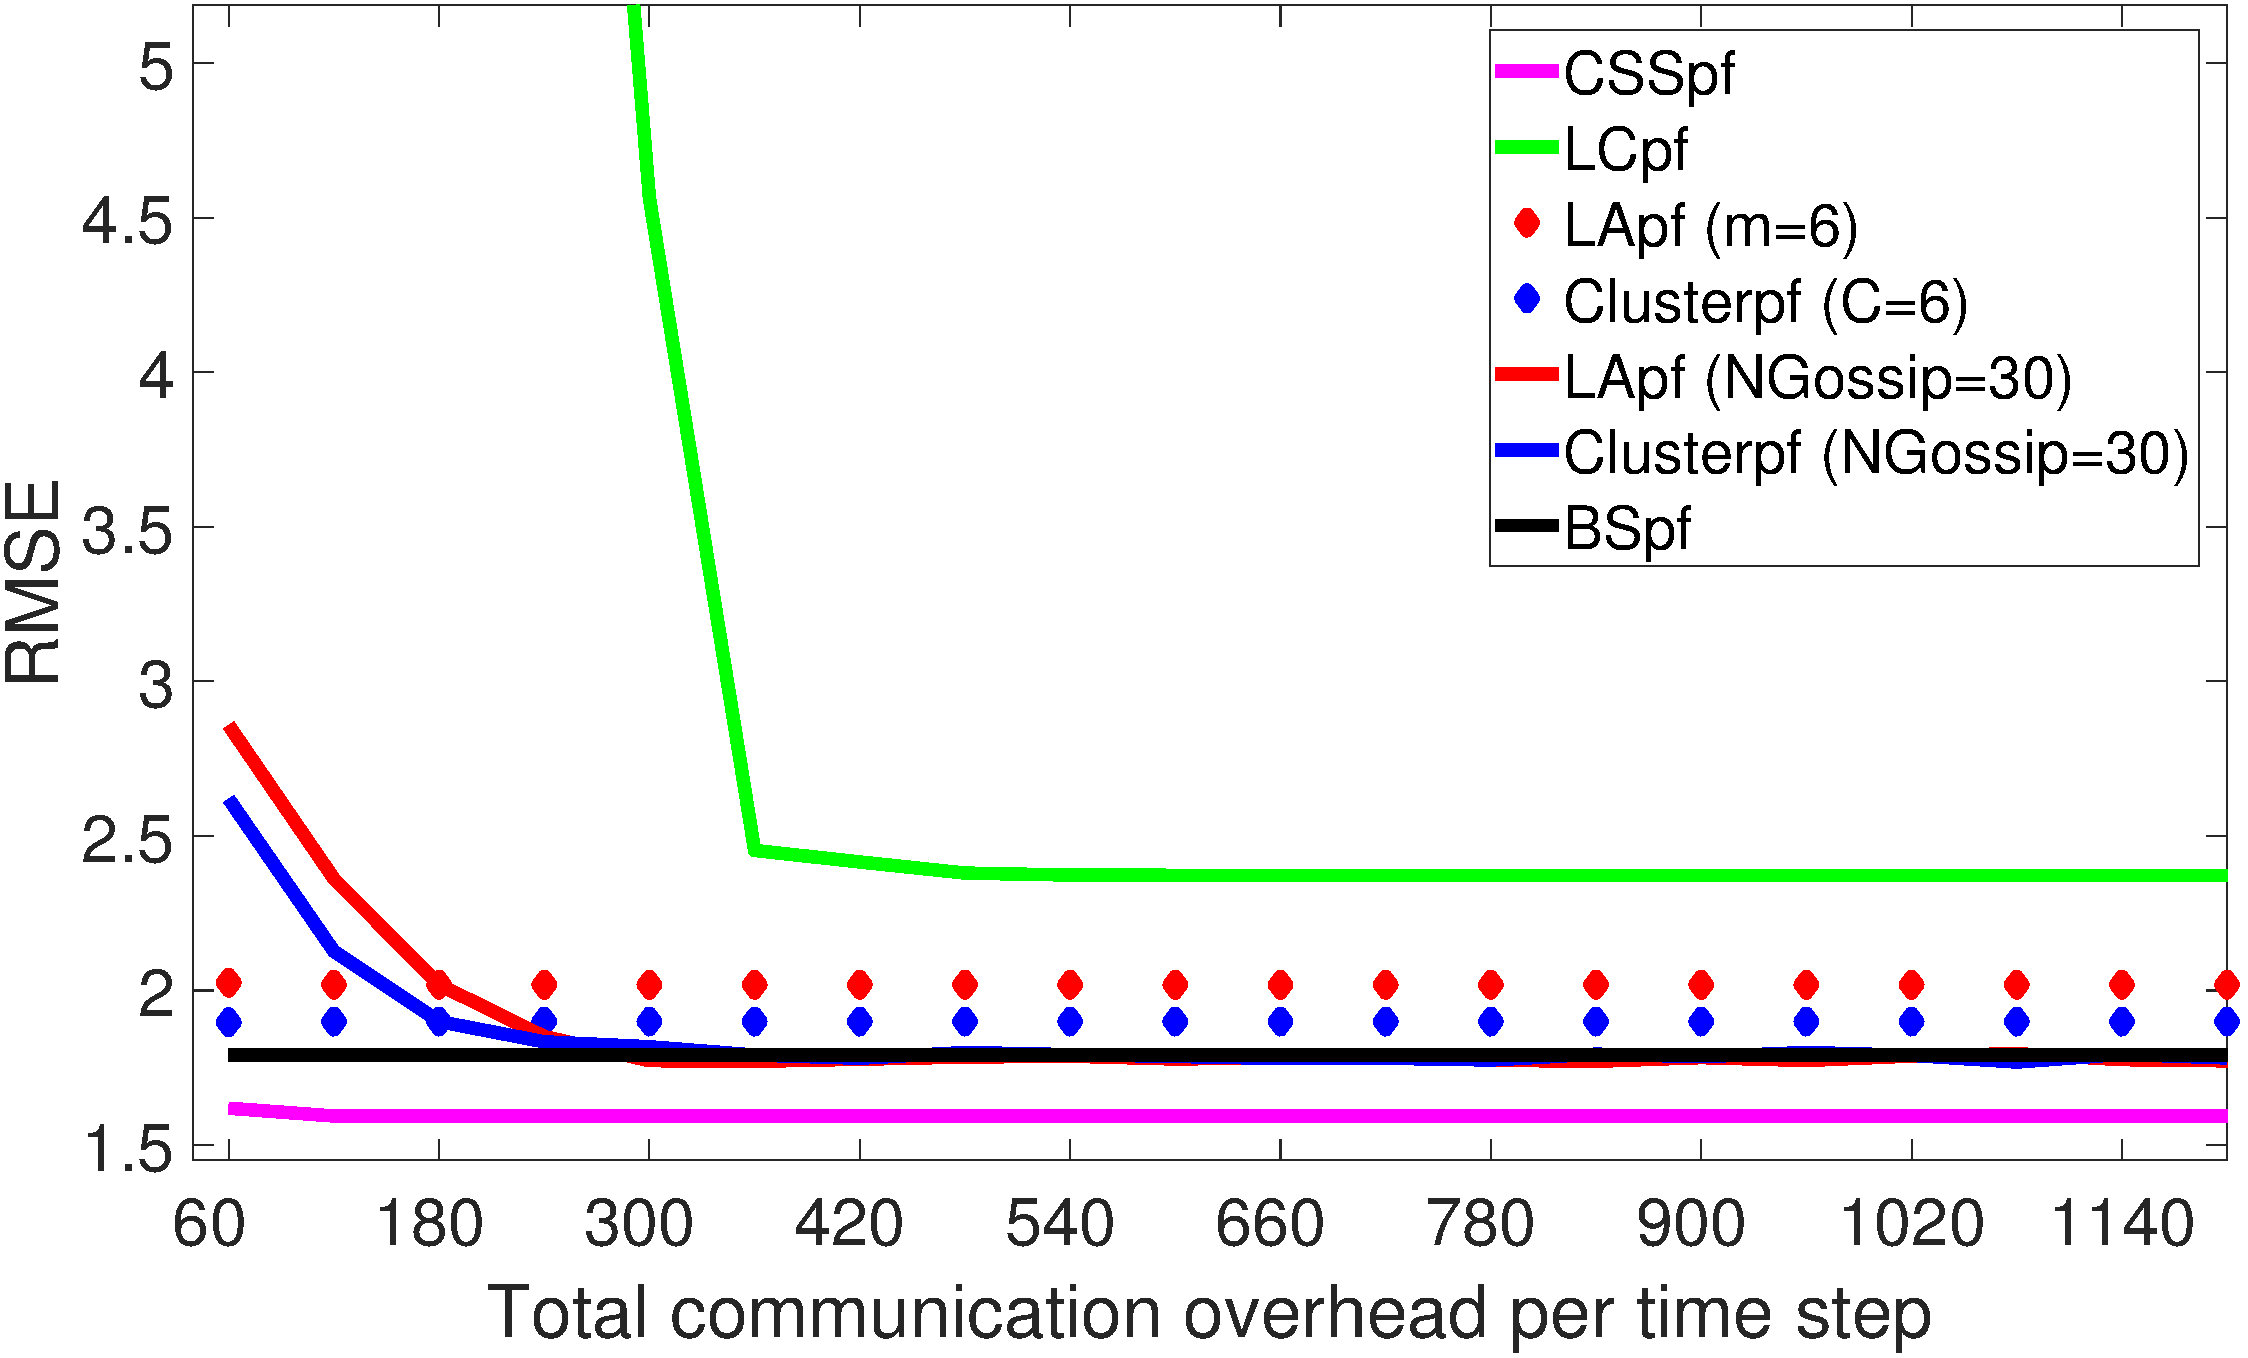
\includegraphics[width=0.65\textwidth]{Figures/Track1_RMSE}}
\end{subfigure}
\begin{subfigure}[total runtime]
{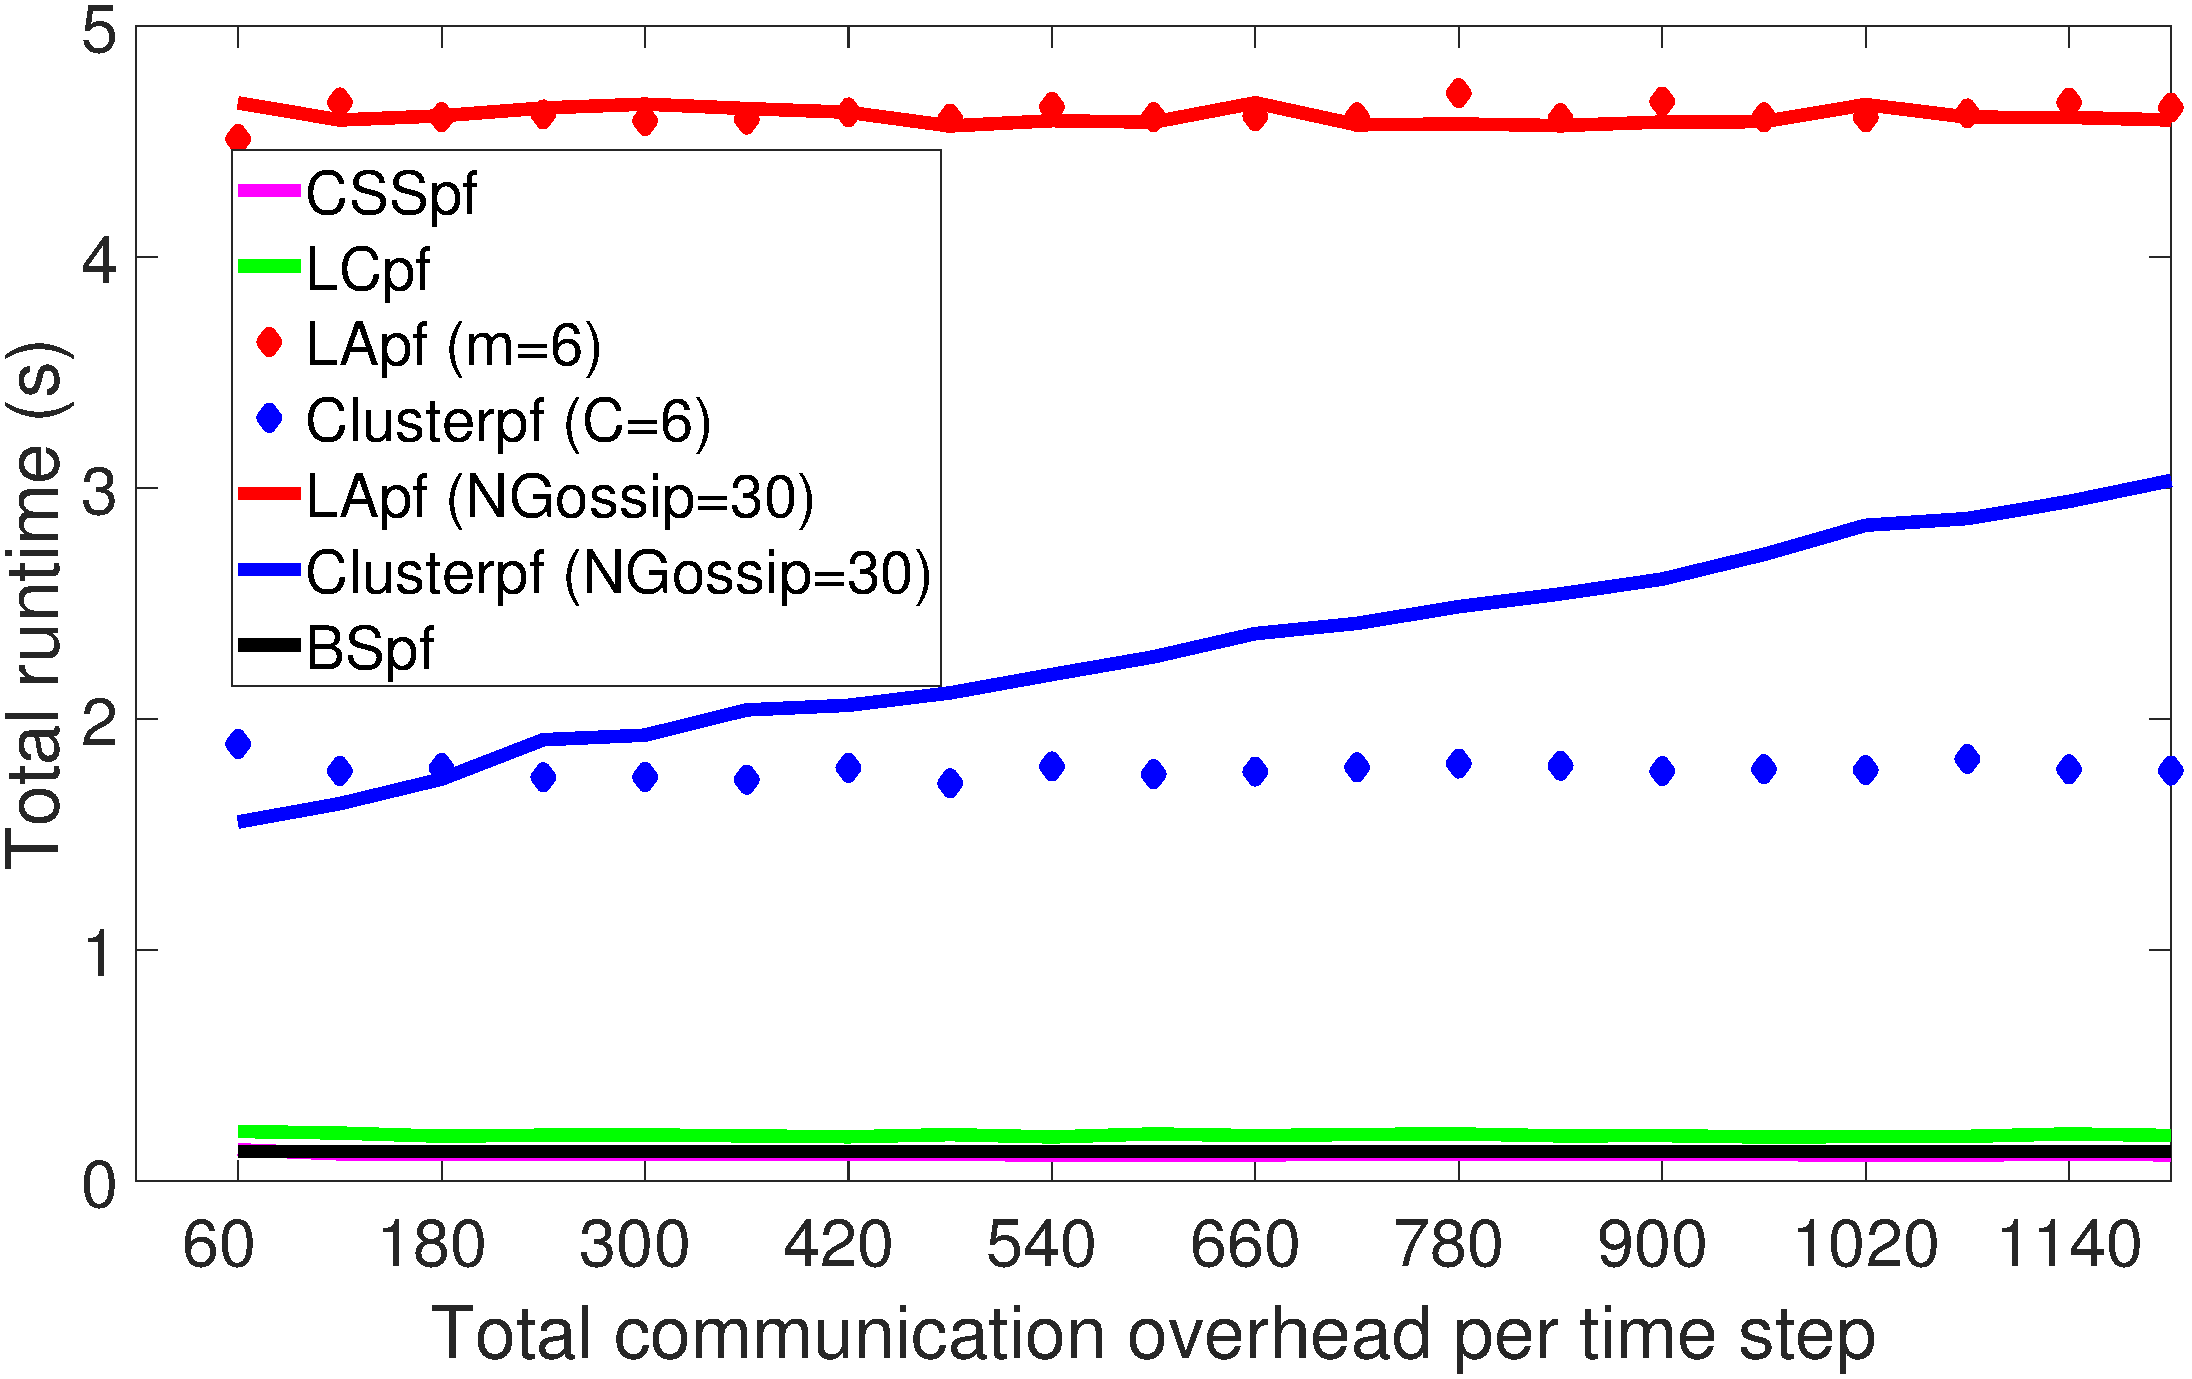
\includegraphics[width=0.65\textwidth]{Figures/Track1_runtime}}
\end{subfigure}
\caption{Average RMSE and runtime with respect to total communication overhead per time step for track 2 ($N=500$, 200 Monte Carlo trials).}
\label{fig:Track1_results}
\end{figure}

Fig.~\ref{fig:Track2_results} shows the tracking results for track 3. Again, the runtime display the same trends as in the previous tracks and we focus solely on RMSE. BSpf has the best performance. LCpf breaks down and loses the target even with the total overhead of 1200 scalars per time step ($NGossip=60$, 20 scalars to aggregate). CSSpf also has a higher break-off point at $NGossip=60$ (comparing to $NGossip=20$ for track 1). When $NGossip$ is fixed, LApf's performance matches that of BSpf $m\geq 5$. Conversely, when $m=6$ is fixed, the RMSE of LApf is fairly consistent over all values of $NGossip$. The same trends can be observed in the two curves of Clusterpf. 

\begin{figure}
\centering
\begin{subfigure}[RMSE]
{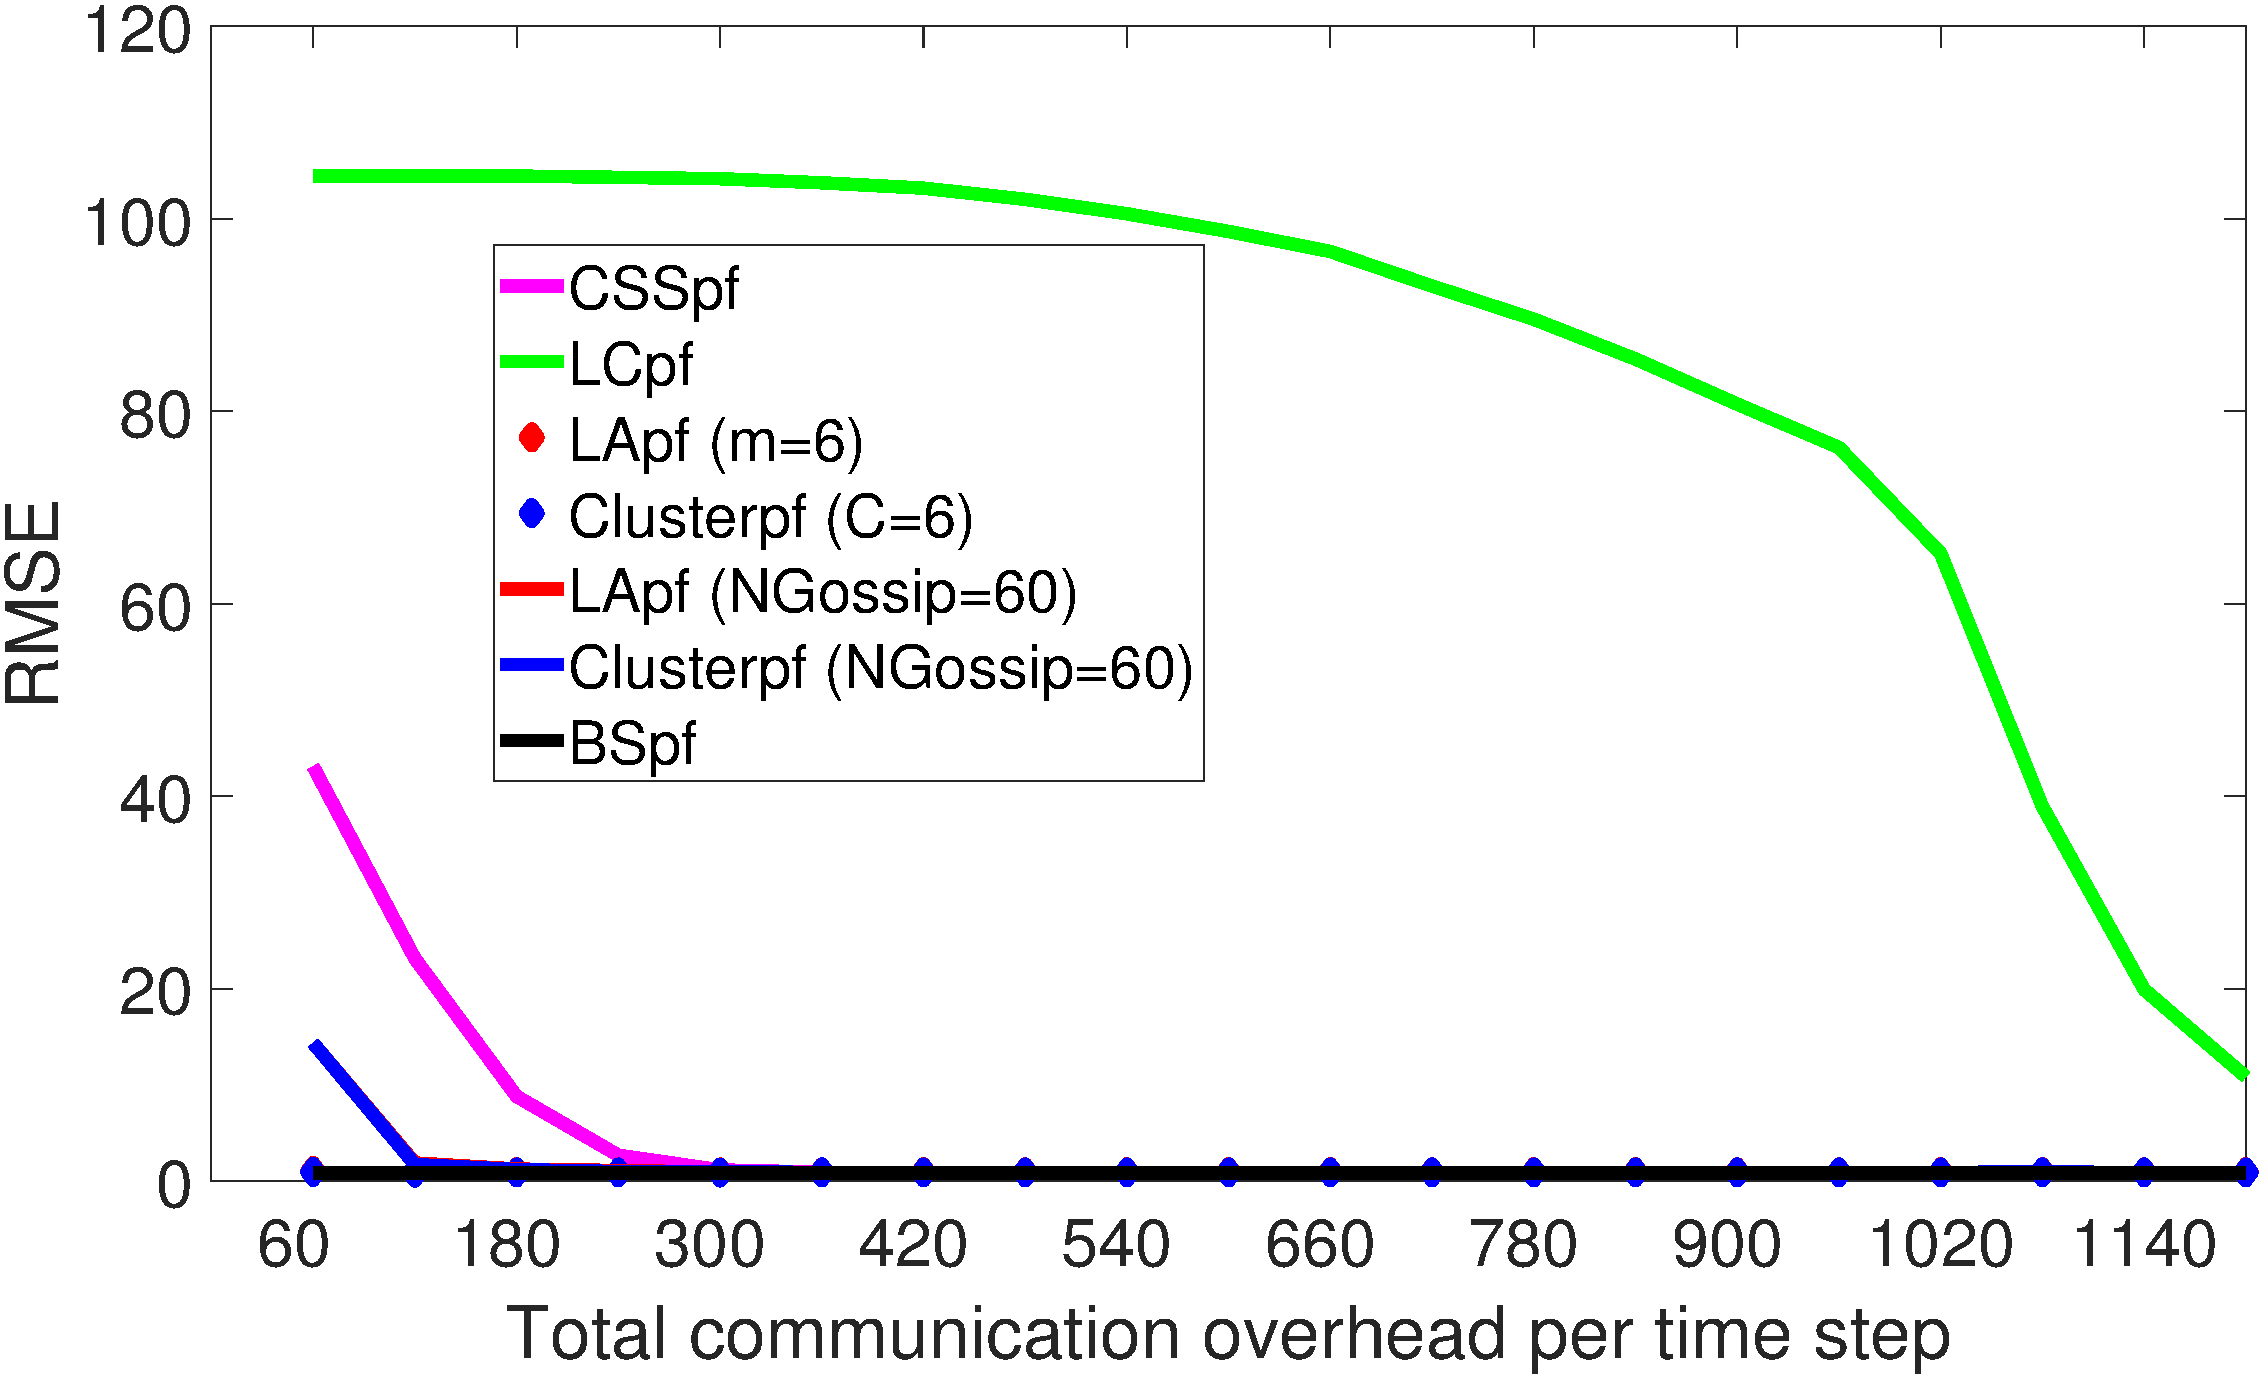
\includegraphics[width=0.65\textwidth]{Figures/Track2_RMSE}}
\end{subfigure}
\begin{subfigure}[RMSE]
{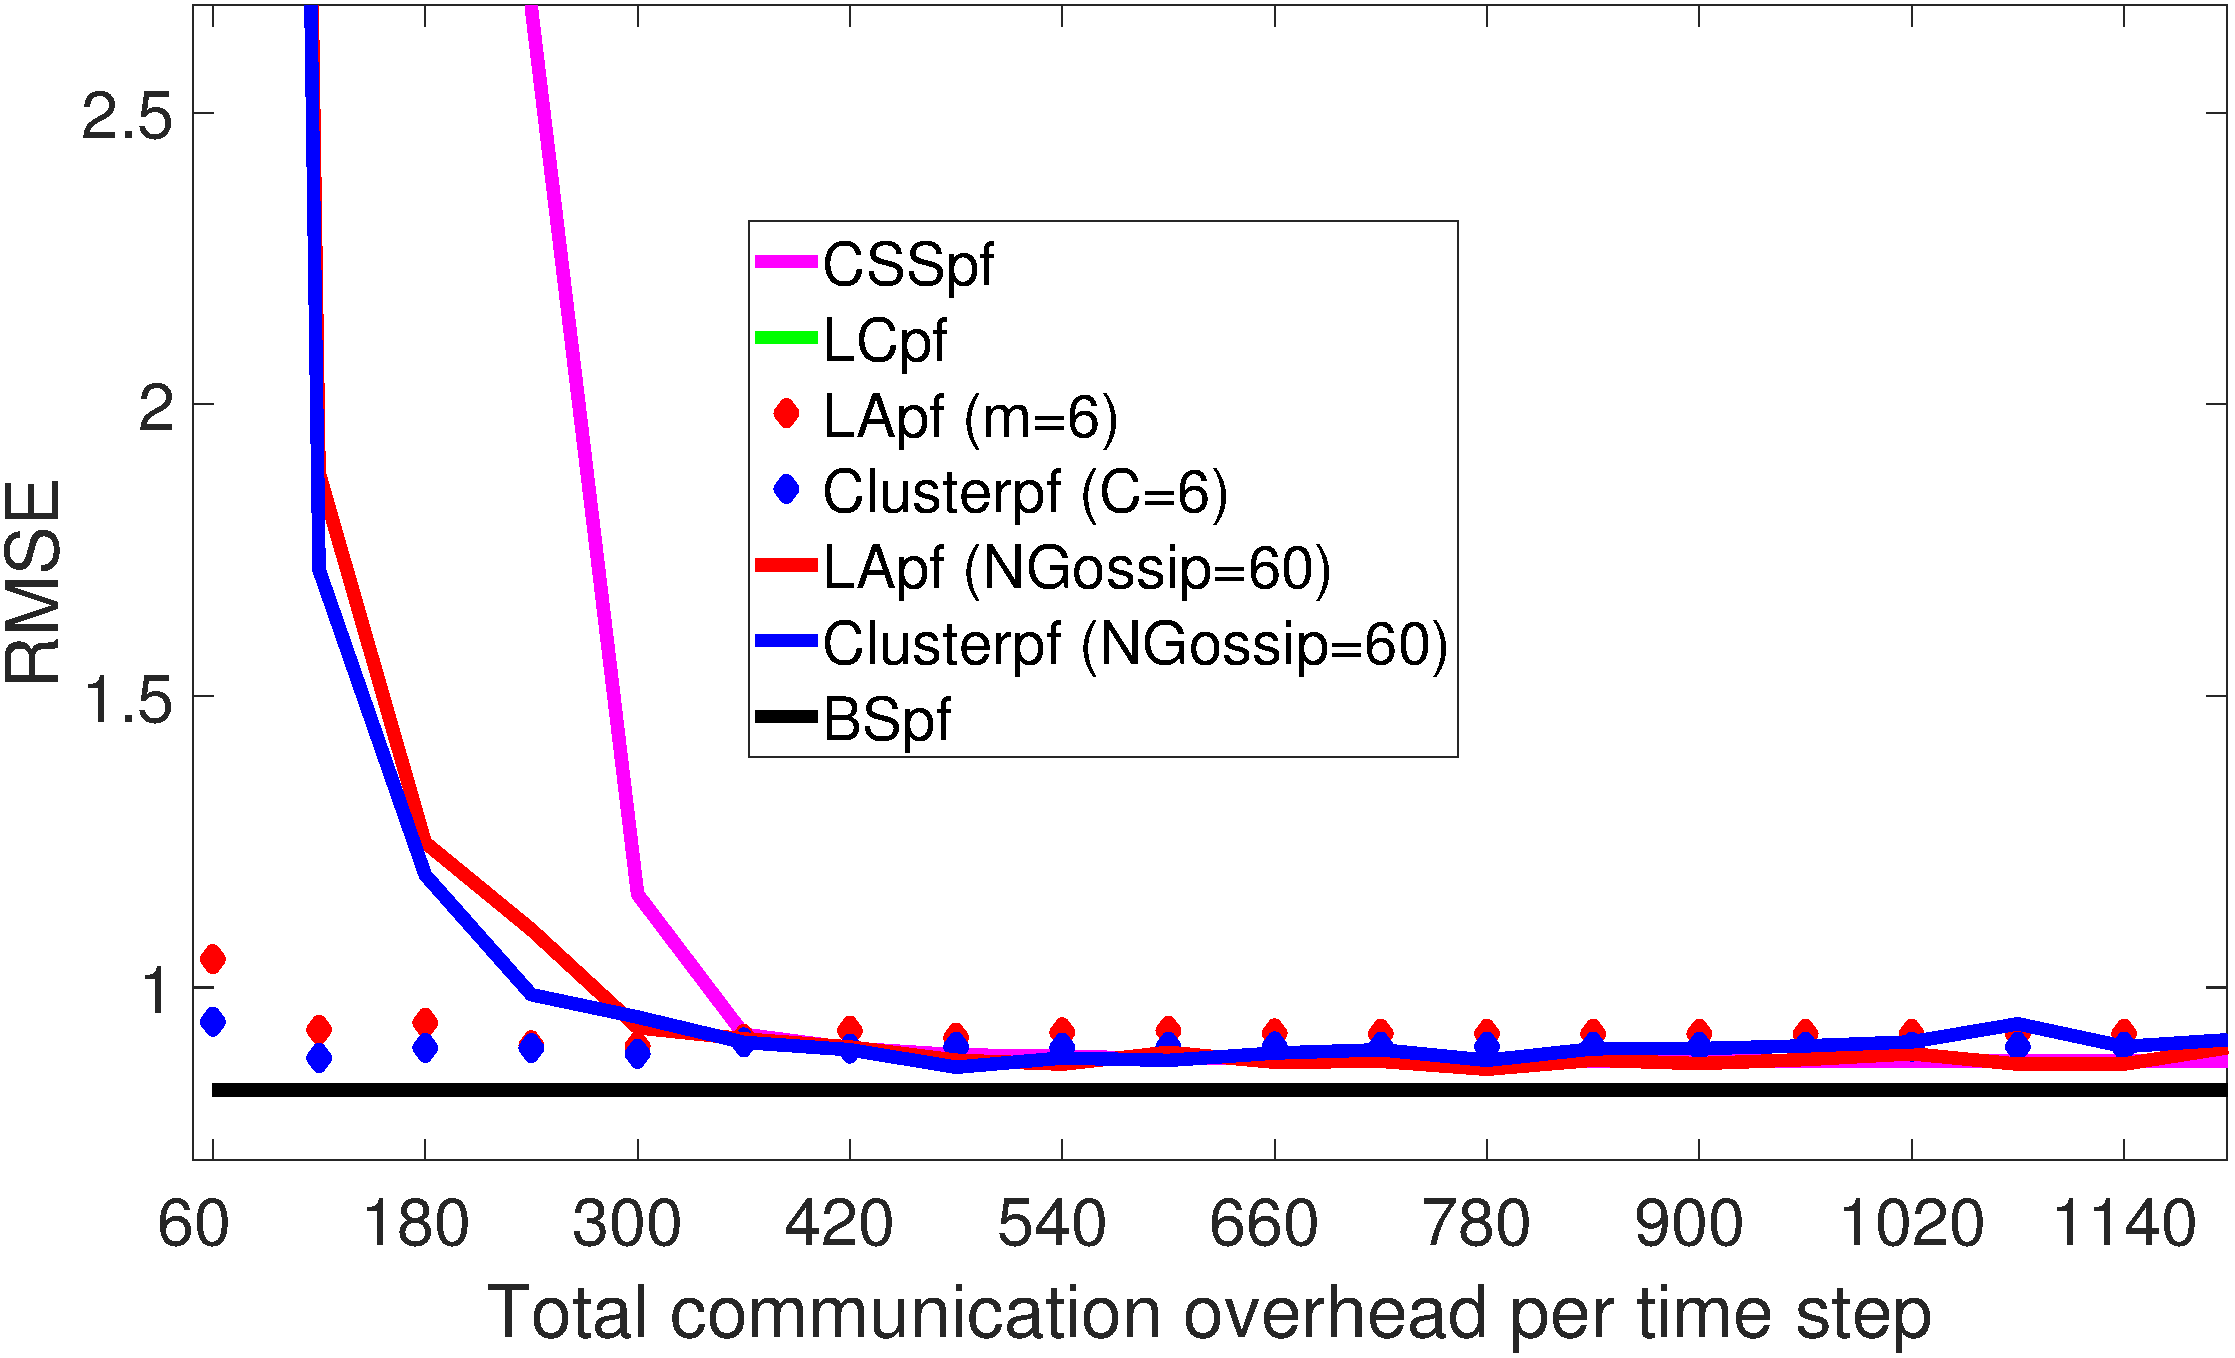
\includegraphics[width=0.65\textwidth]{Figures/Track2_RMSE_focus}}
\end{subfigure}
\begin{subfigure}[total runtime]
{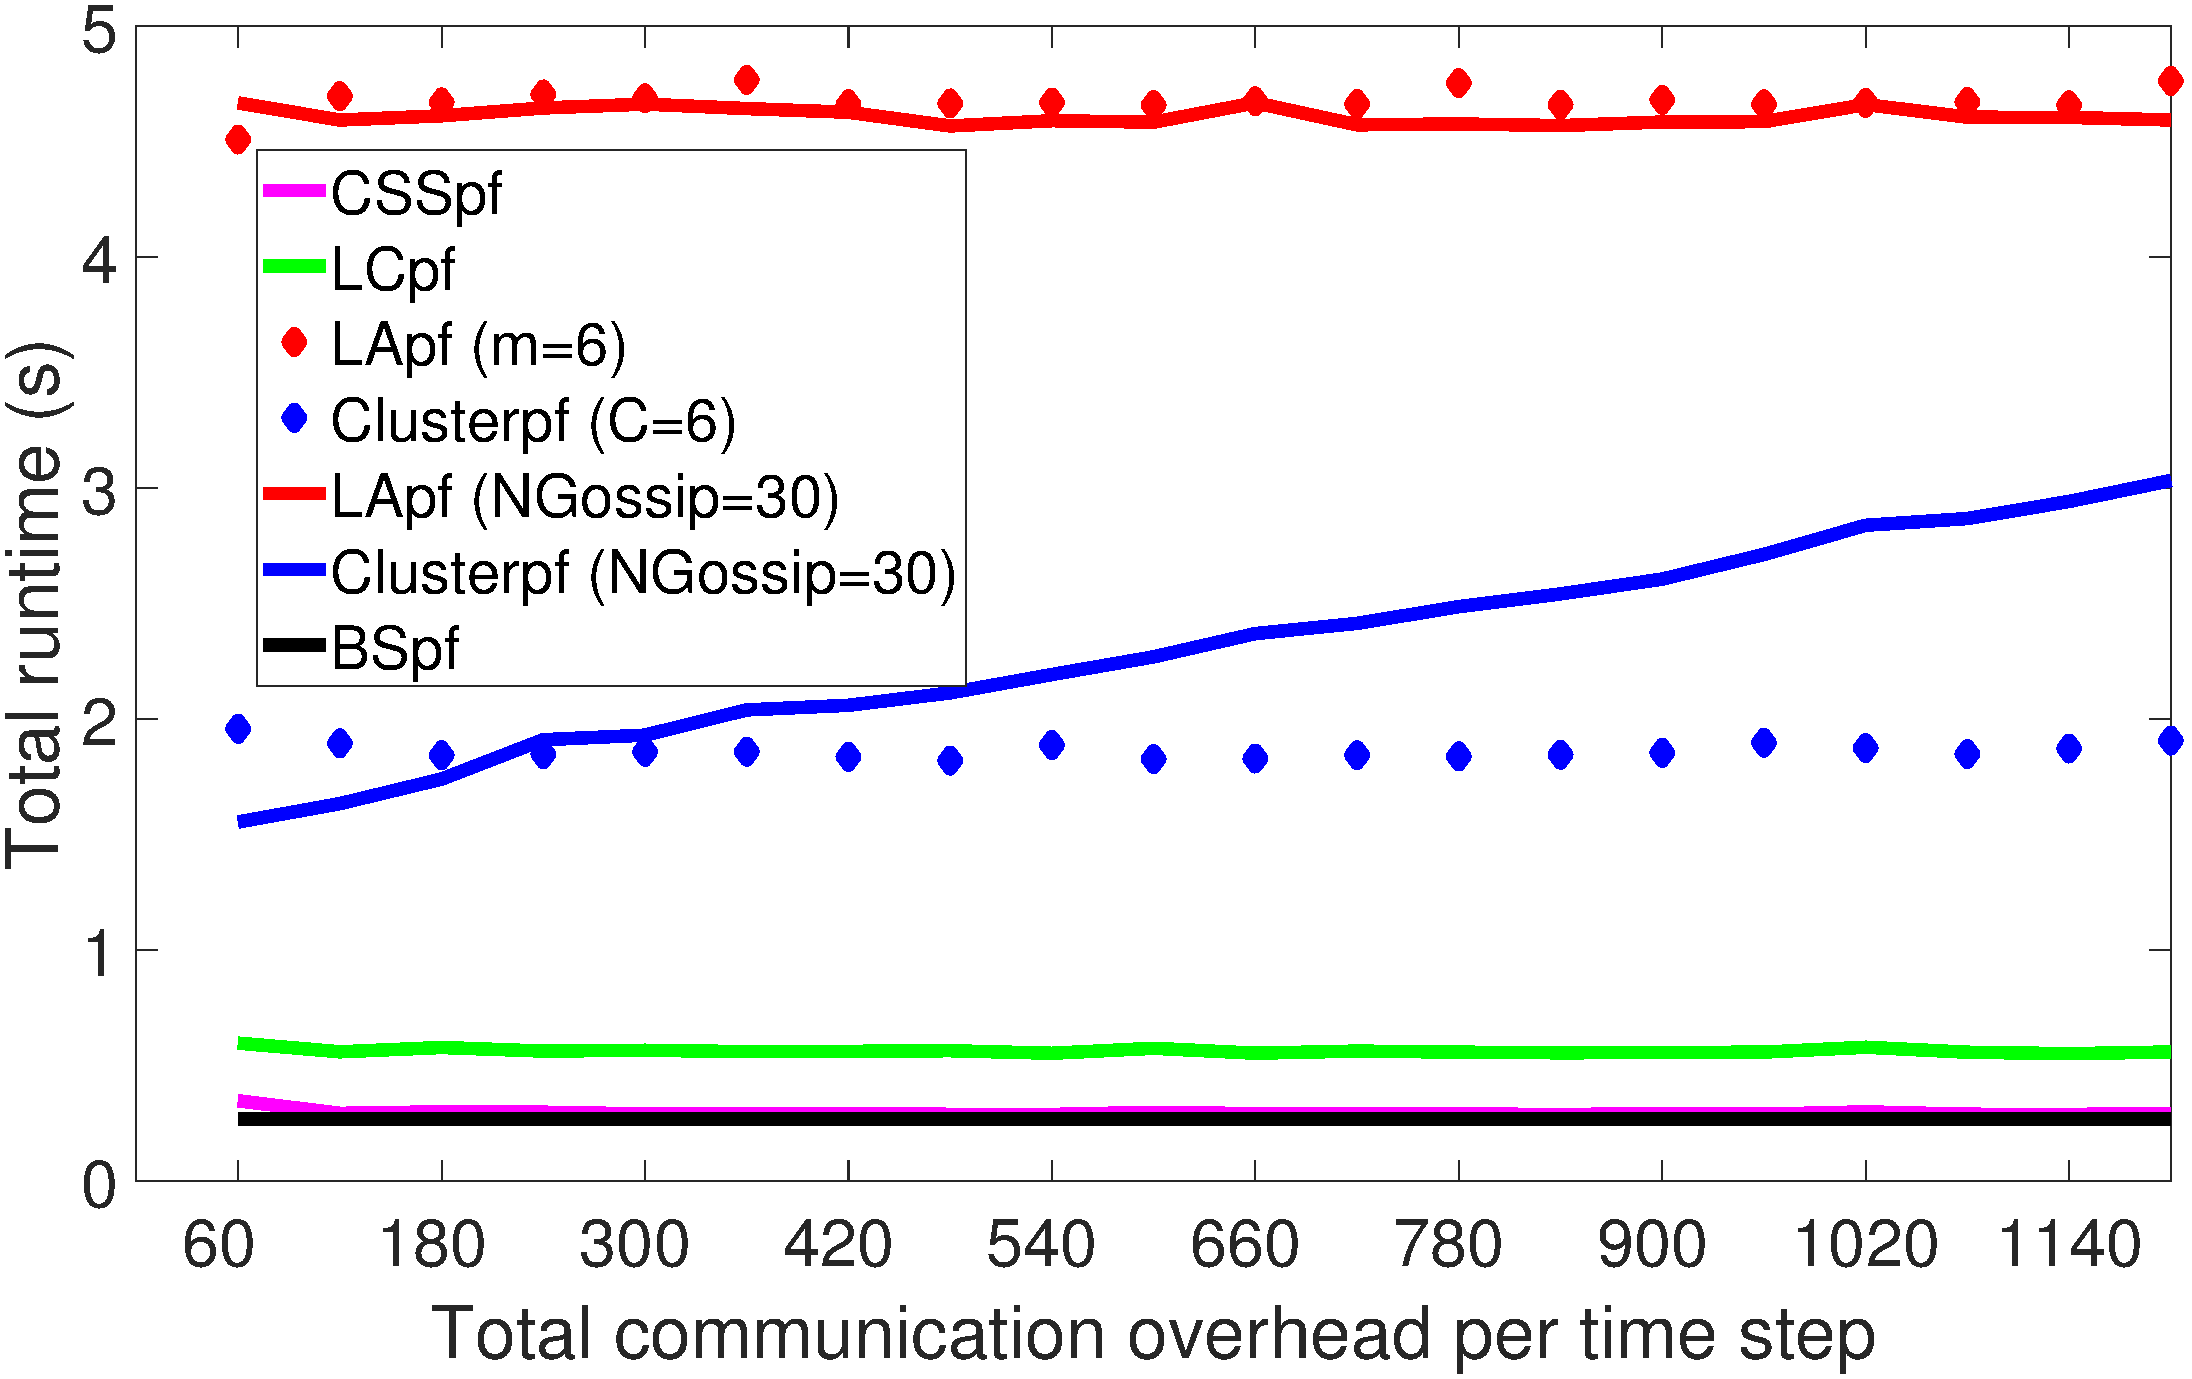
\includegraphics[width=0.65\textwidth]{Figures/Track2_runtime}}
\end{subfigure}
\caption{Average RMSE and runtime with respect to total communication overhead per time step for track 3 ($N=500$, 200 Monte Carlo trials). The subfig b) provides a zoomed view of RMSE curves.}
\label{fig:Track2_results}
\end{figure}

\section{Conclusion}
\label{sec:conclusion}
In this report, we present four distributed particle filters for single-target bearing-only tracking. CSSpf approximates the log-likelihood function using six sufficient statistics. LCpf uses likelihood consensus to approximate the measurement function. LApf constructs a graph over all particles and uses the eigenvectors of resulting Laplacian matrix to encode the particle log-likelihood. Finally, Clusterpf groups particles into clusters, computes the cluster joint log-likelihood and recovers individual particle weights using convex minimization. 

We study each individual algorithm's performance and compare them against each other. The LApf and Clusterpf yield robust tracking performance in all tested scenarios; but they also have the highest runtime by a large margin. LCpf is very fast, but is highly susceptible to gossiping error and requires a much higher communication overhead to achieve adequate tracking performance. Finally, CSSpf is fast but the tracking performance is not always good. 

Out of the three performance criterion, accuracy, runtime and communication overhead, our results suggest the following guidelines. For accuracy and runtime, choose LCpf. For accuracy and communication overhead, choose LApf and Clusterpf. Finally, for runtime and communication overhead, choose CSSpf. 

\bibliographystyle{IEEEtran}
\bibliography{Refs}

\end{document}
